\documentclass[10pt,twocolumn,a4paper]{article}

\usepackage[utf8]{inputenc}
\usepackage[T1]{fontenc}
\usepackage{amsmath,amssymb,amsfonts,amsthm}
\usepackage{graphicx}
\usepackage{booktabs}
\usepackage{multirow}
\usepackage{array}
\usepackage{geometry}
\usepackage{hyperref}
\usepackage{cite}
\usepackage{xcolor}
\usepackage{caption}
\usepackage{enumitem}

% Numbers generated by analysis/make_results_tex.R
% Generated by analysis/make_results_tex.R -- do not edit by hand.
\newcommand{\RaschN}{1000}
\newcommand{\RaschT}{120}
\newcommand{\rSaturnZpdOne}{0.131}
\newcommand{\rSaturnZpdOneLo}{0.128}
\newcommand{\rSaturnZpdOneHi}{0.134}
\newcommand{\rSaturnZpdAOne}{0.128}
\newcommand{\rSaturnZpdAOneLo}{0.126}
\newcommand{\rSaturnZpdAOneHi}{0.131}
\newcommand{\rSaturnZpdCOne}{0.146}
\newcommand{\rSaturnZpdCOneLo}{0.143}
\newcommand{\rSaturnZpdCOneHi}{0.149}
\newcommand{\rSaturnZpdWOne}{0.274}
\newcommand{\rSaturnZpdWOneLo}{0.270}
\newcommand{\rSaturnZpdWOneHi}{0.278}
\newcommand{\rSaturnZpdEOne}{0.195}
\newcommand{\rSaturnZpdEOneLo}{0.192}
\newcommand{\rSaturnZpdEOneHi}{0.199}
\newcommand{\rSaturnBoredOne}{0.234}
\newcommand{\rSaturnBoredOneLo}{0.221}
\newcommand{\rSaturnBoredOneHi}{0.247}
\newcommand{\rSaturnFrustrOne}{0.375}
\newcommand{\rSaturnFrustrOneLo}{0.360}
\newcommand{\rSaturnFrustrOneHi}{0.389}
\newcommand{\rSaturnMeanPOne}{0.494}
\newcommand{\rSaturnMeanPOneLo}{0.481}
\newcommand{\rSaturnMeanPOneHi}{0.506}
\newcommand{\rSaturnGainOne}{-0.032}
\newcommand{\rSaturnGainOneLo}{-0.095}
\newcommand{\rSaturnGainOneHi}{0.031}
\newcommand{\rSaturnTrackOne}{1.869}
\newcommand{\rSaturnTrackOneLo}{1.838}
\newcommand{\rSaturnTrackOneHi}{1.901}
\newcommand{\rFactoryZpdOne}{0.197}
\newcommand{\rFactoryZpdOneLo}{0.177}
\newcommand{\rFactoryZpdOneHi}{0.218}
\newcommand{\rFactoryZpdAOne}{0.166}
\newcommand{\rFactoryZpdAOneLo}{0.151}
\newcommand{\rFactoryZpdAOneHi}{0.182}
\newcommand{\rFactoryZpdCOne}{0.240}
\newcommand{\rFactoryZpdCOneLo}{0.217}
\newcommand{\rFactoryZpdCOneHi}{0.264}
\newcommand{\rFactoryZpdWOne}{0.406}
\newcommand{\rFactoryZpdWOneLo}{0.379}
\newcommand{\rFactoryZpdWOneHi}{0.433}
\newcommand{\rFactoryZpdEOne}{0.269}
\newcommand{\rFactoryZpdEOneLo}{0.247}
\newcommand{\rFactoryZpdEOneHi}{0.292}
\newcommand{\rFactoryBoredOne}{0.287}
\newcommand{\rFactoryBoredOneLo}{0.260}
\newcommand{\rFactoryBoredOneHi}{0.315}
\newcommand{\rFactoryFrustrOne}{0.161}
\newcommand{\rFactoryFrustrOneLo}{0.143}
\newcommand{\rFactoryFrustrOneHi}{0.180}
\newcommand{\rFactoryMeanPOne}{0.636}
\newcommand{\rFactoryMeanPOneLo}{0.620}
\newcommand{\rFactoryMeanPOneHi}{0.652}
\newcommand{\rFactoryGainOne}{0.650}
\newcommand{\rFactoryGainOneLo}{0.571}
\newcommand{\rFactoryGainOneHi}{0.729}
\newcommand{\rFactoryTrackOne}{1.486}
\newcommand{\rFactoryTrackOneLo}{1.429}
\newcommand{\rFactoryTrackOneHi}{1.545}
\newcommand{\rCAT50ZpdOne}{0.472}
\newcommand{\rCAT50ZpdOneLo}{0.460}
\newcommand{\rCAT50ZpdOneHi}{0.484}
\newcommand{\rCAT50ZpdAOne}{0.684}
\newcommand{\rCAT50ZpdAOneLo}{0.675}
\newcommand{\rCAT50ZpdAOneHi}{0.693}
\newcommand{\rCAT50ZpdCOne}{0.155}
\newcommand{\rCAT50ZpdCOneLo}{0.147}
\newcommand{\rCAT50ZpdCOneHi}{0.162}
\newcommand{\rCAT50ZpdWOne}{0.839}
\newcommand{\rCAT50ZpdWOneLo}{0.830}
\newcommand{\rCAT50ZpdWOneHi}{0.847}
\newcommand{\rCAT50ZpdEOne}{0.817}
\newcommand{\rCAT50ZpdEOneLo}{0.809}
\newcommand{\rCAT50ZpdEOneHi}{0.825}
\newcommand{\rCAT50BoredOne}{0.002}
\newcommand{\rCAT50BoredOneLo}{0.001}
\newcommand{\rCAT50BoredOneHi}{0.003}
\newcommand{\rCAT50FrustrOne}{0.027}
\newcommand{\rCAT50FrustrOneLo}{0.024}
\newcommand{\rCAT50FrustrOneHi}{0.031}
\newcommand{\rCAT50MeanPOne}{0.501}
\newcommand{\rCAT50MeanPOneLo}{0.497}
\newcommand{\rCAT50MeanPOneHi}{0.503}
\newcommand{\rCAT50GainOne}{-0.002}
\newcommand{\rCAT50GainOneLo}{-0.013}
\newcommand{\rCAT50GainOneHi}{0.007}
\newcommand{\rCAT50TrackOne}{0.340}
\newcommand{\rCAT50TrackOneLo}{0.333}
\newcommand{\rCAT50TrackOneHi}{0.346}
\newcommand{\rCAT70ZpdOne}{0.335}
\newcommand{\rCAT70ZpdOneLo}{0.323}
\newcommand{\rCAT70ZpdOneHi}{0.348}
\newcommand{\rCAT70ZpdAOne}{0.075}
\newcommand{\rCAT70ZpdAOneLo}{0.069}
\newcommand{\rCAT70ZpdAOneHi}{0.081}
\newcommand{\rCAT70ZpdCOne}{0.740}
\newcommand{\rCAT70ZpdCOneLo}{0.730}
\newcommand{\rCAT70ZpdCOneHi}{0.750}
\newcommand{\rCAT70ZpdWOne}{0.815}
\newcommand{\rCAT70ZpdWOneLo}{0.804}
\newcommand{\rCAT70ZpdWOneHi}{0.825}
\newcommand{\rCAT70ZpdEOne}{0.348}
\newcommand{\rCAT70ZpdEOneLo}{0.335}
\newcommand{\rCAT70ZpdEOneHi}{0.361}
\newcommand{\rCAT70BoredOne}{0.049}
\newcommand{\rCAT70BoredOneLo}{0.043}
\newcommand{\rCAT70BoredOneHi}{0.054}
\newcommand{\rCAT70FrustrOne}{0.002}
\newcommand{\rCAT70FrustrOneLo}{0.001}
\newcommand{\rCAT70FrustrOneHi}{0.003}
\newcommand{\rCAT70MeanPOne}{0.723}
\newcommand{\rCAT70MeanPOneLo}{0.720}
\newcommand{\rCAT70MeanPOneHi}{0.726}
\newcommand{\rCAT70GainOne}{1.078}
\newcommand{\rCAT70GainOneLo}{1.067}
\newcommand{\rCAT70GainOneHi}{1.088}
\newcommand{\rCAT70TrackOne}{1.016}
\newcommand{\rCAT70TrackOneLo}{1.001}
\newcommand{\rCAT70TrackOneHi}{1.031}
\newcommand{\rCAT85ZpdOne}{0.013}
\newcommand{\rCAT85ZpdOneLo}{0.011}
\newcommand{\rCAT85ZpdOneHi}{0.015}
\newcommand{\rCAT85ZpdAOne}{0.004}
\newcommand{\rCAT85ZpdAOneLo}{0.003}
\newcommand{\rCAT85ZpdAOneHi}{0.005}
\newcommand{\rCAT85ZpdCOne}{0.058}
\newcommand{\rCAT85ZpdCOneLo}{0.052}
\newcommand{\rCAT85ZpdCOneHi}{0.064}
\newcommand{\rCAT85ZpdWOne}{0.062}
\newcommand{\rCAT85ZpdWOneLo}{0.056}
\newcommand{\rCAT85ZpdWOneHi}{0.068}
\newcommand{\rCAT85ZpdEOne}{0.014}
\newcommand{\rCAT85ZpdEOneLo}{0.012}
\newcommand{\rCAT85ZpdEOneHi}{0.017}
\newcommand{\rCAT85BoredOne}{0.825}
\newcommand{\rCAT85BoredOneLo}{0.813}
\newcommand{\rCAT85BoredOneHi}{0.836}
\newcommand{\rCAT85FrustrOne}{0.000}
\newcommand{\rCAT85FrustrOneLo}{0.000}
\newcommand{\rCAT85FrustrOneHi}{0.000}
\newcommand{\rCAT85MeanPOne}{0.887}
\newcommand{\rCAT85MeanPOneLo}{0.885}
\newcommand{\rCAT85MeanPOneHi}{0.890}
\newcommand{\rCAT85GainOne}{1.851}
\newcommand{\rCAT85GainOneLo}{1.841}
\newcommand{\rCAT85GainOneHi}{1.861}
\newcommand{\rCAT85TrackOne}{2.175}
\newcommand{\rCAT85TrackOneLo}{2.152}
\newcommand{\rCAT85TrackOneHi}{2.198}
\newcommand{\rCATZpdOne}{0.335}
\newcommand{\rCATZpdOneLo}{0.323}
\newcommand{\rCATZpdOneHi}{0.347}
\newcommand{\rCATZpdAOne}{0.075}
\newcommand{\rCATZpdAOneLo}{0.069}
\newcommand{\rCATZpdAOneHi}{0.081}
\newcommand{\rCATZpdCOne}{0.740}
\newcommand{\rCATZpdCOneLo}{0.730}
\newcommand{\rCATZpdCOneHi}{0.750}
\newcommand{\rCATZpdWOne}{0.815}
\newcommand{\rCATZpdWOneLo}{0.805}
\newcommand{\rCATZpdWOneHi}{0.825}
\newcommand{\rCATZpdEOne}{0.348}
\newcommand{\rCATZpdEOneLo}{0.335}
\newcommand{\rCATZpdEOneHi}{0.360}
\newcommand{\rCATBoredOne}{0.049}
\newcommand{\rCATBoredOneLo}{0.043}
\newcommand{\rCATBoredOneHi}{0.054}
\newcommand{\rCATFrustrOne}{0.002}
\newcommand{\rCATFrustrOneLo}{0.001}
\newcommand{\rCATFrustrOneHi}{0.003}
\newcommand{\rCATMeanPOne}{0.723}
\newcommand{\rCATMeanPOneLo}{0.720}
\newcommand{\rCATMeanPOneHi}{0.726}
\newcommand{\rCATGainOne}{1.078}
\newcommand{\rCATGainOneLo}{1.067}
\newcommand{\rCATGainOneHi}{1.089}
\newcommand{\rCATTrackOne}{1.016}
\newcommand{\rCATTrackOneLo}{1.001}
\newcommand{\rCATTrackOneHi}{1.031}
\newcommand{\rPFPZpdOne}{0.278}
\newcommand{\rPFPZpdOneLo}{0.265}
\newcommand{\rPFPZpdOneHi}{0.292}
\newcommand{\rPFPZpdAOne}{0.296}
\newcommand{\rPFPZpdAOneLo}{0.284}
\newcommand{\rPFPZpdAOneHi}{0.309}
\newcommand{\rPFPZpdCOne}{0.240}
\newcommand{\rPFPZpdCOneLo}{0.225}
\newcommand{\rPFPZpdCOneHi}{0.255}
\newcommand{\rPFPZpdWOne}{0.536}
\newcommand{\rPFPZpdWOneLo}{0.516}
\newcommand{\rPFPZpdWOneHi}{0.556}
\newcommand{\rPFPZpdEOne}{0.428}
\newcommand{\rPFPZpdEOneLo}{0.410}
\newcommand{\rPFPZpdEOneHi}{0.446}
\newcommand{\rPFPBoredOne}{0.061}
\newcommand{\rPFPBoredOneLo}{0.051}
\newcommand{\rPFPBoredOneHi}{0.072}
\newcommand{\rPFPFrustrOne}{0.223}
\newcommand{\rPFPFrustrOneLo}{0.203}
\newcommand{\rPFPFrustrOneHi}{0.242}
\newcommand{\rPFPMeanPOne}{0.496}
\newcommand{\rPFPMeanPOneLo}{0.483}
\newcommand{\rPFPMeanPOneHi}{0.508}
\newcommand{\rPFPGainOne}{-0.022}
\newcommand{\rPFPGainOneLo}{-0.084}
\newcommand{\rPFPGainOneHi}{0.041}
\newcommand{\rPFPTrackOne}{0.892}
\newcommand{\rPFPTrackOneLo}{0.858}
\newcommand{\rPFPTrackOneHi}{0.928}
\newcommand{\rSaturnZpdTwo}{0.139}
\newcommand{\rSaturnZpdTwoLo}{0.137}
\newcommand{\rSaturnZpdTwoHi}{0.141}
\newcommand{\rSaturnZpdATwo}{0.134}
\newcommand{\rSaturnZpdATwoLo}{0.132}
\newcommand{\rSaturnZpdATwoHi}{0.136}
\newcommand{\rSaturnZpdCTwo}{0.158}
\newcommand{\rSaturnZpdCTwoLo}{0.155}
\newcommand{\rSaturnZpdCTwoHi}{0.160}
\newcommand{\rSaturnZpdWTwo}{0.292}
\newcommand{\rSaturnZpdWTwoLo}{0.289}
\newcommand{\rSaturnZpdWTwoHi}{0.295}
\newcommand{\rSaturnZpdETwo}{0.207}
\newcommand{\rSaturnZpdETwoLo}{0.204}
\newcommand{\rSaturnZpdETwoHi}{0.209}
\newcommand{\rSaturnBoredTwo}{0.243}
\newcommand{\rSaturnBoredTwoLo}{0.234}
\newcommand{\rSaturnBoredTwoHi}{0.254}
\newcommand{\rSaturnFrustrTwo}{0.338}
\newcommand{\rSaturnFrustrTwoLo}{0.327}
\newcommand{\rSaturnFrustrTwoHi}{0.349}
\newcommand{\rSaturnMeanPTwo}{0.520}
\newcommand{\rSaturnMeanPTwoLo}{0.511}
\newcommand{\rSaturnMeanPTwoHi}{0.530}
\newcommand{\rSaturnGainTwo}{0.342}
\newcommand{\rSaturnGainTwoLo}{0.339}
\newcommand{\rSaturnGainTwoHi}{0.346}
\newcommand{\rSaturnTrackTwo}{1.682}
\newcommand{\rSaturnTrackTwoLo}{1.666}
\newcommand{\rSaturnTrackTwoHi}{1.701}
\newcommand{\rFactoryZpdTwo}{0.346}
\newcommand{\rFactoryZpdTwoLo}{0.322}
\newcommand{\rFactoryZpdTwoHi}{0.370}
\newcommand{\rFactoryZpdATwo}{0.269}
\newcommand{\rFactoryZpdATwoLo}{0.246}
\newcommand{\rFactoryZpdATwoHi}{0.291}
\newcommand{\rFactoryZpdCTwo}{0.384}
\newcommand{\rFactoryZpdCTwoLo}{0.361}
\newcommand{\rFactoryZpdCTwoHi}{0.409}
\newcommand{\rFactoryZpdWTwo}{0.654}
\newcommand{\rFactoryZpdWTwoLo}{0.630}
\newcommand{\rFactoryZpdWTwoHi}{0.679}
\newcommand{\rFactoryZpdETwo}{0.455}
\newcommand{\rFactoryZpdETwoLo}{0.428}
\newcommand{\rFactoryZpdETwoHi}{0.481}
\newcommand{\rFactoryBoredTwo}{0.119}
\newcommand{\rFactoryBoredTwoLo}{0.103}
\newcommand{\rFactoryBoredTwoHi}{0.136}
\newcommand{\rFactoryFrustrTwo}{0.074}
\newcommand{\rFactoryFrustrTwoLo}{0.060}
\newcommand{\rFactoryFrustrTwoHi}{0.089}
\newcommand{\rFactoryMeanPTwo}{0.625}
\newcommand{\rFactoryMeanPTwoLo}{0.614}
\newcommand{\rFactoryMeanPTwoHi}{0.637}
\newcommand{\rFactoryGainTwo}{0.468}
\newcommand{\rFactoryGainTwoLo}{0.459}
\newcommand{\rFactoryGainTwoHi}{0.476}
\newcommand{\rFactoryTrackTwo}{0.941}
\newcommand{\rFactoryTrackTwoLo}{0.902}
\newcommand{\rFactoryTrackTwoHi}{0.984}
\newcommand{\rCAT50ZpdTwo}{0.524}
\newcommand{\rCAT50ZpdTwoLo}{0.513}
\newcommand{\rCAT50ZpdTwoHi}{0.535}
\newcommand{\rCAT50ZpdATwo}{0.664}
\newcommand{\rCAT50ZpdATwoLo}{0.656}
\newcommand{\rCAT50ZpdATwoHi}{0.671}
\newcommand{\rCAT50ZpdCTwo}{0.200}
\newcommand{\rCAT50ZpdCTwoLo}{0.191}
\newcommand{\rCAT50ZpdCTwoHi}{0.209}
\newcommand{\rCAT50ZpdWTwo}{0.864}
\newcommand{\rCAT50ZpdWTwoLo}{0.857}
\newcommand{\rCAT50ZpdWTwoHi}{0.870}
\newcommand{\rCAT50ZpdETwo}{0.832}
\newcommand{\rCAT50ZpdETwoLo}{0.826}
\newcommand{\rCAT50ZpdETwoHi}{0.839}
\newcommand{\rCAT50BoredTwo}{0.002}
\newcommand{\rCAT50BoredTwoLo}{0.001}
\newcommand{\rCAT50BoredTwoHi}{0.003}
\newcommand{\rCAT50FrustrTwo}{0.022}
\newcommand{\rCAT50FrustrTwoLo}{0.020}
\newcommand{\rCAT50FrustrTwoHi}{0.025}
\newcommand{\rCAT50MeanPTwo}{0.515}
\newcommand{\rCAT50MeanPTwoLo}{0.512}
\newcommand{\rCAT50MeanPTwoHi}{0.518}
\newcommand{\rCAT50GainTwo}{0.571}
\newcommand{\rCAT50GainTwoLo}{0.568}
\newcommand{\rCAT50GainTwoHi}{0.575}
\newcommand{\rCAT50TrackTwo}{0.349}
\newcommand{\rCAT50TrackTwoLo}{0.343}
\newcommand{\rCAT50TrackTwoHi}{0.355}
\newcommand{\rCAT70ZpdTwo}{0.406}
\newcommand{\rCAT70ZpdTwoLo}{0.395}
\newcommand{\rCAT70ZpdTwoHi}{0.417}
\newcommand{\rCAT70ZpdATwo}{0.102}
\newcommand{\rCAT70ZpdATwoLo}{0.096}
\newcommand{\rCAT70ZpdATwoHi}{0.109}
\newcommand{\rCAT70ZpdCTwo}{0.750}
\newcommand{\rCAT70ZpdCTwoLo}{0.742}
\newcommand{\rCAT70ZpdCTwoHi}{0.758}
\newcommand{\rCAT70ZpdWTwo}{0.852}
\newcommand{\rCAT70ZpdWTwoLo}{0.844}
\newcommand{\rCAT70ZpdWTwoHi}{0.861}
\newcommand{\rCAT70ZpdETwo}{0.421}
\newcommand{\rCAT70ZpdETwoLo}{0.409}
\newcommand{\rCAT70ZpdETwoHi}{0.434}
\newcommand{\rCAT70BoredTwo}{0.038}
\newcommand{\rCAT70BoredTwoLo}{0.034}
\newcommand{\rCAT70BoredTwoHi}{0.042}
\newcommand{\rCAT70FrustrTwo}{0.002}
\newcommand{\rCAT70FrustrTwoLo}{0.001}
\newcommand{\rCAT70FrustrTwoHi}{0.002}
\newcommand{\rCAT70MeanPTwo}{0.709}
\newcommand{\rCAT70MeanPTwoLo}{0.706}
\newcommand{\rCAT70MeanPTwoHi}{0.712}
\newcommand{\rCAT70GainTwo}{0.477}
\newcommand{\rCAT70GainTwoLo}{0.473}
\newcommand{\rCAT70GainTwoHi}{0.481}
\newcommand{\rCAT70TrackTwo}{0.944}
\newcommand{\rCAT70TrackTwoLo}{0.932}
\newcommand{\rCAT70TrackTwoHi}{0.957}
\newcommand{\rCAT85ZpdTwo}{0.017}
\newcommand{\rCAT85ZpdTwoLo}{0.015}
\newcommand{\rCAT85ZpdTwoHi}{0.020}
\newcommand{\rCAT85ZpdATwo}{0.004}
\newcommand{\rCAT85ZpdATwoLo}{0.003}
\newcommand{\rCAT85ZpdATwoHi}{0.005}
\newcommand{\rCAT85ZpdCTwo}{0.142}
\newcommand{\rCAT85ZpdCTwoLo}{0.132}
\newcommand{\rCAT85ZpdCTwoHi}{0.152}
\newcommand{\rCAT85ZpdWTwo}{0.147}
\newcommand{\rCAT85ZpdWTwoLo}{0.137}
\newcommand{\rCAT85ZpdWTwoHi}{0.156}
\newcommand{\rCAT85ZpdETwo}{0.019}
\newcommand{\rCAT85ZpdETwoLo}{0.016}
\newcommand{\rCAT85ZpdETwoHi}{0.021}
\newcommand{\rCAT85BoredTwo}{0.602}
\newcommand{\rCAT85BoredTwoLo}{0.586}
\newcommand{\rCAT85BoredTwoHi}{0.618}
\newcommand{\rCAT85FrustrTwo}{0.000}
\newcommand{\rCAT85FrustrTwoLo}{0.000}
\newcommand{\rCAT85FrustrTwoHi}{0.000}
\newcommand{\rCAT85MeanPTwo}{0.855}
\newcommand{\rCAT85MeanPTwoLo}{0.853}
\newcommand{\rCAT85MeanPTwoHi}{0.857}
\newcommand{\rCAT85GainTwo}{0.288}
\newcommand{\rCAT85GainTwoLo}{0.284}
\newcommand{\rCAT85GainTwoHi}{0.292}
\newcommand{\rCAT85TrackTwo}{1.861}
\newcommand{\rCAT85TrackTwoLo}{1.842}
\newcommand{\rCAT85TrackTwoHi}{1.879}
\newcommand{\rCATZpdTwo}{0.406}
\newcommand{\rCATZpdTwoLo}{0.394}
\newcommand{\rCATZpdTwoHi}{0.418}
\newcommand{\rCATZpdATwo}{0.102}
\newcommand{\rCATZpdATwoLo}{0.096}
\newcommand{\rCATZpdATwoHi}{0.108}
\newcommand{\rCATZpdCTwo}{0.750}
\newcommand{\rCATZpdCTwoLo}{0.742}
\newcommand{\rCATZpdCTwoHi}{0.758}
\newcommand{\rCATZpdWTwo}{0.852}
\newcommand{\rCATZpdWTwoLo}{0.844}
\newcommand{\rCATZpdWTwoHi}{0.860}
\newcommand{\rCATZpdETwo}{0.421}
\newcommand{\rCATZpdETwoLo}{0.409}
\newcommand{\rCATZpdETwoHi}{0.433}
\newcommand{\rCATBoredTwo}{0.038}
\newcommand{\rCATBoredTwoLo}{0.034}
\newcommand{\rCATBoredTwoHi}{0.042}
\newcommand{\rCATFrustrTwo}{0.002}
\newcommand{\rCATFrustrTwoLo}{0.001}
\newcommand{\rCATFrustrTwoHi}{0.002}
\newcommand{\rCATMeanPTwo}{0.709}
\newcommand{\rCATMeanPTwoLo}{0.706}
\newcommand{\rCATMeanPTwoHi}{0.712}
\newcommand{\rCATGainTwo}{0.477}
\newcommand{\rCATGainTwoLo}{0.472}
\newcommand{\rCATGainTwoHi}{0.480}
\newcommand{\rCATTrackTwo}{0.944}
\newcommand{\rCATTrackTwoLo}{0.932}
\newcommand{\rCATTrackTwoHi}{0.958}
\newcommand{\rPFPZpdTwo}{0.374}
\newcommand{\rPFPZpdTwoLo}{0.362}
\newcommand{\rPFPZpdTwoHi}{0.386}
\newcommand{\rPFPZpdATwo}{0.366}
\newcommand{\rPFPZpdATwoLo}{0.354}
\newcommand{\rPFPZpdATwoHi}{0.377}
\newcommand{\rPFPZpdCTwo}{0.313}
\newcommand{\rPFPZpdCTwoLo}{0.299}
\newcommand{\rPFPZpdCTwoHi}{0.327}
\newcommand{\rPFPZpdWTwo}{0.678}
\newcommand{\rPFPZpdWTwoLo}{0.663}
\newcommand{\rPFPZpdWTwoHi}{0.695}
\newcommand{\rPFPZpdETwo}{0.546}
\newcommand{\rPFPZpdETwoLo}{0.532}
\newcommand{\rPFPZpdETwoHi}{0.559}
\newcommand{\rPFPBoredTwo}{0.032}
\newcommand{\rPFPBoredTwoLo}{0.026}
\newcommand{\rPFPBoredTwoHi}{0.039}
\newcommand{\rPFPFrustrTwo}{0.116}
\newcommand{\rPFPFrustrTwoLo}{0.103}
\newcommand{\rPFPFrustrTwoHi}{0.128}
\newcommand{\rPFPMeanPTwo}{0.535}
\newcommand{\rPFPMeanPTwoLo}{0.526}
\newcommand{\rPFPMeanPTwoHi}{0.544}
\newcommand{\rPFPGainTwo}{0.516}
\newcommand{\rPFPGainTwoLo}{0.510}
\newcommand{\rPFPGainTwoHi}{0.521}
\newcommand{\rPFPTrackTwo}{0.687}
\newcommand{\rPFPTrackTwoLo}{0.666}
\newcommand{\rPFPTrackTwoHi}{0.709}
\newcommand{\cSaturnZpdOne}{+0.147}
\newcommand{\cSaturnZpdOneLo}{+0.134}
\newcommand{\cSaturnZpdOneHi}{+0.160}
\newcommand{\cSaturnZpdOneDz}{+0.71}
\newcommand{\cSaturnZpdAOne}{+0.168}
\newcommand{\cSaturnZpdAOneLo}{+0.156}
\newcommand{\cSaturnZpdAOneHi}{+0.181}
\newcommand{\cSaturnZpdAOneDz}{+0.84}
\newcommand{\cSaturnZpdCOne}{+0.094}
\newcommand{\cSaturnZpdCOneLo}{+0.079}
\newcommand{\cSaturnZpdCOneHi}{+0.108}
\newcommand{\cSaturnZpdCOneDz}{+0.41}
\newcommand{\cSaturnZpdWOne}{+0.262}
\newcommand{\cSaturnZpdWOneLo}{+0.244}
\newcommand{\cSaturnZpdWOneHi}{+0.280}
\newcommand{\cSaturnZpdWOneDz}{+0.89}
\newcommand{\cSaturnZpdEOne}{+0.232}
\newcommand{\cSaturnZpdEOneLo}{+0.216}
\newcommand{\cSaturnZpdEOneHi}{+0.249}
\newcommand{\cSaturnZpdEOneDz}{+0.89}
\newcommand{\cSaturnBoredOne}{-0.172}
\newcommand{\cSaturnBoredOneLo}{-0.181}
\newcommand{\cSaturnBoredOneHi}{-0.163}
\newcommand{\cSaturnBoredOneDz}{-1.18}
\newcommand{\cSaturnFrustrOne}{-0.152}
\newcommand{\cSaturnFrustrOneLo}{-0.162}
\newcommand{\cSaturnFrustrOneHi}{-0.143}
\newcommand{\cSaturnFrustrOneDz}{-0.98}
\newcommand{\cSaturnMeanPOne}{+0.002}
\newcommand{\cSaturnMeanPOneLo}{-0.001}
\newcommand{\cSaturnMeanPOneHi}{+0.004}
\newcommand{\cSaturnMeanPOneDz}{+0.04}
\newcommand{\cSaturnGainOne}{+0.010}
\newcommand{\cSaturnGainOneLo}{-0.006}
\newcommand{\cSaturnGainOneHi}{+0.026}
\newcommand{\cSaturnGainOneDz}{+0.04}
\newcommand{\cSaturnTrackOne}{-0.977}
\newcommand{\cSaturnTrackOneLo}{-0.988}
\newcommand{\cSaturnTrackOneHi}{-0.967}
\newcommand{\cSaturnTrackOneDz}{-5.53}
\newcommand{\cFactoryZpdOne}{+0.081}
\newcommand{\cFactoryZpdOneLo}{+0.056}
\newcommand{\cFactoryZpdOneHi}{+0.105}
\newcommand{\cFactoryZpdOneDz}{+0.21}
\newcommand{\cFactoryZpdAOne}{+0.130}
\newcommand{\cFactoryZpdAOneLo}{+0.112}
\newcommand{\cFactoryZpdAOneHi}{+0.147}
\newcommand{\cFactoryZpdAOneDz}{+0.45}
\newcommand{\cFactoryZpdCOne}{+0.000}
\newcommand{\cFactoryZpdCOneLo}{-0.026}
\newcommand{\cFactoryZpdCOneHi}{+0.027}
\newcommand{\cFactoryZpdCOneDz}{+0.00}
\newcommand{\cFactoryZpdWOne}{+0.130}
\newcommand{\cFactoryZpdWOneLo}{+0.101}
\newcommand{\cFactoryZpdWOneHi}{+0.162}
\newcommand{\cFactoryZpdWOneDz}{+0.27}
\newcommand{\cFactoryZpdEOne}{+0.159}
\newcommand{\cFactoryZpdEOneLo}{+0.130}
\newcommand{\cFactoryZpdEOneHi}{+0.185}
\newcommand{\cFactoryZpdEOneDz}{+0.37}
\newcommand{\cFactoryBoredOne}{-0.226}
\newcommand{\cFactoryBoredOneLo}{-0.248}
\newcommand{\cFactoryBoredOneHi}{-0.205}
\newcommand{\cFactoryBoredOneDz}{-0.63}
\newcommand{\cFactoryFrustrOne}{+0.062}
\newcommand{\cFactoryFrustrOneLo}{+0.056}
\newcommand{\cFactoryFrustrOneHi}{+0.067}
\newcommand{\cFactoryFrustrOneDz}{+0.67}
\newcommand{\cFactoryMeanPOne}{-0.141}
\newcommand{\cFactoryMeanPOneLo}{-0.146}
\newcommand{\cFactoryMeanPOneHi}{-0.135}
\newcommand{\cFactoryMeanPOneDz}{-1.54}
\newcommand{\cFactoryGainOne}{-0.672}
\newcommand{\cFactoryGainOneLo}{-0.700}
\newcommand{\cFactoryGainOneHi}{-0.642}
\newcommand{\cFactoryGainOneDz}{-1.42}
\newcommand{\cFactoryTrackOne}{-0.594}
\newcommand{\cFactoryTrackOneLo}{-0.634}
\newcommand{\cFactoryTrackOneHi}{-0.554}
\newcommand{\cFactoryTrackOneDz}{-0.93}
\newcommand{\cCAT50ZpdOne}{-0.194}
\newcommand{\cCAT50ZpdOneLo}{-0.209}
\newcommand{\cCAT50ZpdOneHi}{-0.180}
\newcommand{\cCAT50ZpdOneDz}{-0.80}
\newcommand{\cCAT50ZpdAOne}{-0.388}
\newcommand{\cCAT50ZpdAOneLo}{-0.400}
\newcommand{\cCAT50ZpdAOneHi}{-0.376}
\newcommand{\cCAT50ZpdAOneDz}{-1.93}
\newcommand{\cCAT50ZpdCOne}{+0.085}
\newcommand{\cCAT50ZpdCOneLo}{+0.071}
\newcommand{\cCAT50ZpdCOneHi}{+0.100}
\newcommand{\cCAT50ZpdCOneDz}{+0.38}
\newcommand{\cCAT50ZpdWOne}{-0.303}
\newcommand{\cCAT50ZpdWOneLo}{-0.321}
\newcommand{\cCAT50ZpdWOneHi}{-0.285}
\newcommand{\cCAT50ZpdWOneDz}{-1.05}
\newcommand{\cCAT50ZpdEOne}{-0.389}
\newcommand{\cCAT50ZpdEOneLo}{-0.404}
\newcommand{\cCAT50ZpdEOneHi}{-0.373}
\newcommand{\cCAT50ZpdEOneDz}{-1.56}
\newcommand{\cCAT50BoredOne}{+0.059}
\newcommand{\cCAT50BoredOneLo}{+0.050}
\newcommand{\cCAT50BoredOneHi}{+0.070}
\newcommand{\cCAT50BoredOneDz}{+0.37}
\newcommand{\cCAT50FrustrOne}{+0.196}
\newcommand{\cCAT50FrustrOneLo}{+0.180}
\newcommand{\cCAT50FrustrOneHi}{+0.213}
\newcommand{\cCAT50FrustrOneDz}{+0.72}
\newcommand{\cCAT50MeanPOne}{-0.005}
\newcommand{\cCAT50MeanPOneLo}{-0.016}
\newcommand{\cCAT50MeanPOneHi}{+0.006}
\newcommand{\cCAT50MeanPOneDz}{-0.03}
\newcommand{\cCAT50GainOne}{-0.020}
\newcommand{\cCAT50GainOneLo}{-0.072}
\newcommand{\cCAT50GainOneHi}{+0.032}
\newcommand{\cCAT50GainOneDz}{-0.02}
\newcommand{\cCAT50TrackOne}{+0.553}
\newcommand{\cCAT50TrackOneLo}{+0.522}
\newcommand{\cCAT50TrackOneHi}{+0.582}
\newcommand{\cCAT50TrackOneDz}{+1.11}
\newcommand{\cCAT70ZpdOne}{-0.057}
\newcommand{\cCAT70ZpdOneLo}{-0.077}
\newcommand{\cCAT70ZpdOneHi}{-0.038}
\newcommand{\cCAT70ZpdOneDz}{-0.18}
\newcommand{\cCAT70ZpdAOne}{+0.221}
\newcommand{\cCAT70ZpdAOneLo}{+0.206}
\newcommand{\cCAT70ZpdAOneHi}{+0.236}
\newcommand{\cCAT70ZpdAOneDz}{+0.91}
\newcommand{\cCAT70ZpdCOne}{-0.500}
\newcommand{\cCAT70ZpdCOneLo}{-0.518}
\newcommand{\cCAT70ZpdCOneHi}{-0.483}
\newcommand{\cCAT70ZpdCOneDz}{-1.72}
\newcommand{\cCAT70ZpdWOne}{-0.279}
\newcommand{\cCAT70ZpdWOneLo}{-0.302}
\newcommand{\cCAT70ZpdWOneHi}{-0.256}
\newcommand{\cCAT70ZpdWOneDz}{-0.76}
\newcommand{\cCAT70ZpdEOne}{+0.080}
\newcommand{\cCAT70ZpdEOneLo}{+0.058}
\newcommand{\cCAT70ZpdEOneHi}{+0.103}
\newcommand{\cCAT70ZpdEOneDz}{+0.22}
\newcommand{\cCAT70BoredOne}{+0.013}
\newcommand{\cCAT70BoredOneLo}{+0.006}
\newcommand{\cCAT70BoredOneHi}{+0.021}
\newcommand{\cCAT70BoredOneDz}{+0.10}
\newcommand{\cCAT70FrustrOne}{+0.221}
\newcommand{\cCAT70FrustrOneLo}{+0.202}
\newcommand{\cCAT70FrustrOneHi}{+0.241}
\newcommand{\cCAT70FrustrOneDz}{+0.73}
\newcommand{\cCAT70MeanPOne}{-0.227}
\newcommand{\cCAT70MeanPOneLo}{-0.238}
\newcommand{\cCAT70MeanPOneHi}{-0.217}
\newcommand{\cCAT70MeanPOneDz}{-1.32}
\newcommand{\cCAT70GainOne}{-1.100}
\newcommand{\cCAT70GainOneLo}{-1.153}
\newcommand{\cCAT70GainOneHi}{-1.048}
\newcommand{\cCAT70GainOneDz}{-1.31}
\newcommand{\cCAT70TrackOne}{-0.124}
\newcommand{\cCAT70TrackOneLo}{-0.158}
\newcommand{\cCAT70TrackOneHi}{-0.090}
\newcommand{\cCAT70TrackOneDz}{-0.22}
\newcommand{\cCAT85ZpdOne}{+0.265}
\newcommand{\cCAT85ZpdOneLo}{+0.250}
\newcommand{\cCAT85ZpdOneHi}{+0.280}
\newcommand{\cCAT85ZpdOneDz}{+1.13}
\newcommand{\cCAT85ZpdAOne}{+0.292}
\newcommand{\cCAT85ZpdAOneLo}{+0.278}
\newcommand{\cCAT85ZpdAOneHi}{+0.305}
\newcommand{\cCAT85ZpdAOneDz}{+1.37}
\newcommand{\cCAT85ZpdCOne}{+0.182}
\newcommand{\cCAT85ZpdCOneLo}{+0.163}
\newcommand{\cCAT85ZpdCOneHi}{+0.201}
\newcommand{\cCAT85ZpdCOneDz}{+0.61}
\newcommand{\cCAT85ZpdWOne}{+0.474}
\newcommand{\cCAT85ZpdWOneLo}{+0.450}
\newcommand{\cCAT85ZpdWOneHi}{+0.497}
\newcommand{\cCAT85ZpdWOneDz}{+1.20}
\newcommand{\cCAT85ZpdEOne}{+0.413}
\newcommand{\cCAT85ZpdEOneLo}{+0.394}
\newcommand{\cCAT85ZpdEOneHi}{+0.431}
\newcommand{\cCAT85ZpdEOneDz}{+1.38}
\newcommand{\cCAT85BoredOne}{-0.764}
\newcommand{\cCAT85BoredOneLo}{-0.777}
\newcommand{\cCAT85BoredOneHi}{-0.750}
\newcommand{\cCAT85BoredOneDz}{-3.50}
\newcommand{\cCAT85FrustrOne}{+0.223}
\newcommand{\cCAT85FrustrOneLo}{+0.204}
\newcommand{\cCAT85FrustrOneHi}{+0.242}
\newcommand{\cCAT85FrustrOneDz}{+0.72}
\newcommand{\cCAT85MeanPOne}{-0.392}
\newcommand{\cCAT85MeanPOneLo}{-0.402}
\newcommand{\cCAT85MeanPOneHi}{-0.381}
\newcommand{\cCAT85MeanPOneDz}{-2.27}
\newcommand{\cCAT85GainOne}{-1.873}
\newcommand{\cCAT85GainOneLo}{-1.927}
\newcommand{\cCAT85GainOneHi}{-1.820}
\newcommand{\cCAT85GainOneDz}{-2.20}
\newcommand{\cCAT85TrackOne}{-1.282}
\newcommand{\cCAT85TrackOneLo}{-1.320}
\newcommand{\cCAT85TrackOneHi}{-1.244}
\newcommand{\cCAT85TrackOneDz}{-2.09}
\newcommand{\cCATZpdOne}{-0.057}
\newcommand{\cCATZpdOneLo}{-0.077}
\newcommand{\cCATZpdOneHi}{-0.037}
\newcommand{\cCATZpdOneDz}{-0.18}
\newcommand{\cCATZpdAOne}{+0.221}
\newcommand{\cCATZpdAOneLo}{+0.206}
\newcommand{\cCATZpdAOneHi}{+0.236}
\newcommand{\cCATZpdAOneDz}{+0.91}
\newcommand{\cCATZpdCOne}{-0.500}
\newcommand{\cCATZpdCOneLo}{-0.518}
\newcommand{\cCATZpdCOneHi}{-0.483}
\newcommand{\cCATZpdCOneDz}{-1.72}
\newcommand{\cCATZpdWOne}{-0.279}
\newcommand{\cCATZpdWOneLo}{-0.301}
\newcommand{\cCATZpdWOneHi}{-0.256}
\newcommand{\cCATZpdWOneDz}{-0.76}
\newcommand{\cCATZpdEOne}{+0.080}
\newcommand{\cCATZpdEOneLo}{+0.057}
\newcommand{\cCATZpdEOneHi}{+0.101}
\newcommand{\cCATZpdEOneDz}{+0.22}
\newcommand{\cCATBoredOne}{+0.013}
\newcommand{\cCATBoredOneLo}{+0.005}
\newcommand{\cCATBoredOneHi}{+0.021}
\newcommand{\cCATBoredOneDz}{+0.10}
\newcommand{\cCATFrustrOne}{+0.221}
\newcommand{\cCATFrustrOneLo}{+0.202}
\newcommand{\cCATFrustrOneHi}{+0.240}
\newcommand{\cCATFrustrOneDz}{+0.73}
\newcommand{\cCATMeanPOne}{-0.227}
\newcommand{\cCATMeanPOneLo}{-0.238}
\newcommand{\cCATMeanPOneHi}{-0.216}
\newcommand{\cCATMeanPOneDz}{-1.32}
\newcommand{\cCATGainOne}{-1.100}
\newcommand{\cCATGainOneLo}{-1.153}
\newcommand{\cCATGainOneHi}{-1.047}
\newcommand{\cCATGainOneDz}{-1.31}
\newcommand{\cCATTrackOne}{-0.124}
\newcommand{\cCATTrackOneLo}{-0.160}
\newcommand{\cCATTrackOneHi}{-0.087}
\newcommand{\cCATTrackOneDz}{-0.22}
\newcommand{\cSaturnZpdTwo}{+0.235}
\newcommand{\cSaturnZpdTwoLo}{+0.223}
\newcommand{\cSaturnZpdTwoHi}{+0.246}
\newcommand{\cSaturnZpdTwoDz}{+1.23}
\newcommand{\cSaturnZpdATwo}{+0.231}
\newcommand{\cSaturnZpdATwoLo}{+0.220}
\newcommand{\cSaturnZpdATwoHi}{+0.243}
\newcommand{\cSaturnZpdATwoDz}{+1.26}
\newcommand{\cSaturnZpdCTwo}{+0.155}
\newcommand{\cSaturnZpdCTwoLo}{+0.141}
\newcommand{\cSaturnZpdCTwoHi}{+0.169}
\newcommand{\cSaturnZpdCTwoDz}{+0.68}
\newcommand{\cSaturnZpdWTwo}{+0.386}
\newcommand{\cSaturnZpdWTwoLo}{+0.370}
\newcommand{\cSaturnZpdWTwoHi}{+0.402}
\newcommand{\cSaturnZpdWTwoDz}{+1.52}
\newcommand{\cSaturnZpdETwo}{+0.339}
\newcommand{\cSaturnZpdETwoLo}{+0.325}
\newcommand{\cSaturnZpdETwoHi}{+0.353}
\newcommand{\cSaturnZpdETwoDz}{+1.49}
\newcommand{\cSaturnBoredTwo}{-0.211}
\newcommand{\cSaturnBoredTwoLo}{-0.219}
\newcommand{\cSaturnBoredTwoHi}{-0.203}
\newcommand{\cSaturnBoredTwoDz}{-1.62}
\newcommand{\cSaturnFrustrTwo}{-0.222}
\newcommand{\cSaturnFrustrTwoLo}{-0.230}
\newcommand{\cSaturnFrustrTwoHi}{-0.215}
\newcommand{\cSaturnFrustrTwoDz}{-1.74}
\newcommand{\cSaturnMeanPTwo}{+0.015}
\newcommand{\cSaturnMeanPTwoLo}{+0.013}
\newcommand{\cSaturnMeanPTwoHi}{+0.017}
\newcommand{\cSaturnMeanPTwoDz}{+0.50}
\newcommand{\cSaturnGainTwo}{+0.173}
\newcommand{\cSaturnGainTwoLo}{+0.169}
\newcommand{\cSaturnGainTwoHi}{+0.177}
\newcommand{\cSaturnGainTwoDz}{+2.74}
\newcommand{\cSaturnTrackTwo}{-0.995}
\newcommand{\cSaturnTrackTwoLo}{-1.004}
\newcommand{\cSaturnTrackTwoHi}{-0.986}
\newcommand{\cSaturnTrackTwoDz}{-6.94}
\newcommand{\cFactoryZpdTwo}{+0.028}
\newcommand{\cFactoryZpdTwoLo}{+0.006}
\newcommand{\cFactoryZpdTwoHi}{+0.050}
\newcommand{\cFactoryZpdTwoDz}{+0.08}
\newcommand{\cFactoryZpdATwo}{+0.097}
\newcommand{\cFactoryZpdATwoLo}{+0.077}
\newcommand{\cFactoryZpdATwoHi}{+0.115}
\newcommand{\cFactoryZpdATwoDz}{+0.31}
\newcommand{\cFactoryZpdCTwo}{-0.072}
\newcommand{\cFactoryZpdCTwoLo}{-0.094}
\newcommand{\cFactoryZpdCTwoHi}{-0.050}
\newcommand{\cFactoryZpdCTwoDz}{-0.20}
\newcommand{\cFactoryZpdWTwo}{+0.025}
\newcommand{\cFactoryZpdWTwoLo}{+0.004}
\newcommand{\cFactoryZpdWTwoHi}{+0.045}
\newcommand{\cFactoryZpdWTwoDz}{+0.07}
\newcommand{\cFactoryZpdETwo}{+0.091}
\newcommand{\cFactoryZpdETwoLo}{+0.069}
\newcommand{\cFactoryZpdETwoHi}{+0.114}
\newcommand{\cFactoryZpdETwoDz}{+0.25}
\newcommand{\cFactoryBoredTwo}{-0.087}
\newcommand{\cFactoryBoredTwoLo}{-0.100}
\newcommand{\cFactoryBoredTwoHi}{-0.075}
\newcommand{\cFactoryBoredTwoDz}{-0.42}
\newcommand{\cFactoryFrustrTwo}{+0.042}
\newcommand{\cFactoryFrustrTwoLo}{+0.035}
\newcommand{\cFactoryFrustrTwoHi}{+0.049}
\newcommand{\cFactoryFrustrTwoDz}{+0.36}
\newcommand{\cFactoryMeanPTwo}{-0.091}
\newcommand{\cFactoryMeanPTwoLo}{-0.094}
\newcommand{\cFactoryMeanPTwoHi}{-0.088}
\newcommand{\cFactoryMeanPTwoDz}{-1.73}
\newcommand{\cFactoryGainTwo}{+0.048}
\newcommand{\cFactoryGainTwoLo}{+0.043}
\newcommand{\cFactoryGainTwoHi}{+0.054}
\newcommand{\cFactoryGainTwoDz}{+0.57}
\newcommand{\cFactoryTrackTwo}{-0.254}
\newcommand{\cFactoryTrackTwoLo}{-0.278}
\newcommand{\cFactoryTrackTwoHi}{-0.227}
\newcommand{\cFactoryTrackTwoDz}{-0.61}
\newcommand{\cCAT50ZpdTwo}{-0.150}
\newcommand{\cCAT50ZpdTwoLo}{-0.162}
\newcommand{\cCAT50ZpdTwoHi}{-0.137}
\newcommand{\cCAT50ZpdTwoDz}{-0.69}
\newcommand{\cCAT50ZpdATwo}{-0.298}
\newcommand{\cCAT50ZpdATwoLo}{-0.310}
\newcommand{\cCAT50ZpdATwoHi}{-0.287}
\newcommand{\cCAT50ZpdATwoDz}{-1.63}
\newcommand{\cCAT50ZpdCTwo}{+0.113}
\newcommand{\cCAT50ZpdCTwoLo}{+0.100}
\newcommand{\cCAT50ZpdCTwoHi}{+0.126}
\newcommand{\cCAT50ZpdCTwoDz}{+0.51}
\newcommand{\cCAT50ZpdWTwo}{-0.185}
\newcommand{\cCAT50ZpdWTwoLo}{-0.199}
\newcommand{\cCAT50ZpdWTwoHi}{-0.172}
\newcommand{\cCAT50ZpdWTwoDz}{-0.82}
\newcommand{\cCAT50ZpdETwo}{-0.287}
\newcommand{\cCAT50ZpdETwoLo}{-0.299}
\newcommand{\cCAT50ZpdETwoHi}{-0.275}
\newcommand{\cCAT50ZpdETwoDz}{-1.41}
\newcommand{\cCAT50BoredTwo}{+0.030}
\newcommand{\cCAT50BoredTwoLo}{+0.024}
\newcommand{\cCAT50BoredTwoHi}{+0.036}
\newcommand{\cCAT50BoredTwoDz}{+0.31}
\newcommand{\cCAT50FrustrTwo}{+0.093}
\newcommand{\cCAT50FrustrTwoLo}{+0.083}
\newcommand{\cCAT50FrustrTwoHi}{+0.104}
\newcommand{\cCAT50FrustrTwoDz}{+0.55}
\newcommand{\cCAT50MeanPTwo}{+0.020}
\newcommand{\cCAT50MeanPTwoLo}{+0.013}
\newcommand{\cCAT50MeanPTwoHi}{+0.028}
\newcommand{\cCAT50MeanPTwoDz}{+0.16}
\newcommand{\cCAT50GainTwo}{-0.056}
\newcommand{\cCAT50GainTwoLo}{-0.060}
\newcommand{\cCAT50GainTwoHi}{-0.052}
\newcommand{\cCAT50GainTwoDz}{-0.84}
\newcommand{\cCAT50TrackTwo}{+0.338}
\newcommand{\cCAT50TrackTwoLo}{+0.320}
\newcommand{\cCAT50TrackTwoHi}{+0.358}
\newcommand{\cCAT50TrackTwoDz}{+1.14}
\newcommand{\cCAT70ZpdTwo}{-0.032}
\newcommand{\cCAT70ZpdTwoLo}{-0.049}
\newcommand{\cCAT70ZpdTwoHi}{-0.015}
\newcommand{\cCAT70ZpdTwoDz}{-0.12}
\newcommand{\cCAT70ZpdATwo}{+0.263}
\newcommand{\cCAT70ZpdATwoLo}{+0.250}
\newcommand{\cCAT70ZpdATwoHi}{+0.277}
\newcommand{\cCAT70ZpdATwoDz}{+1.26}
\newcommand{\cCAT70ZpdCTwo}{-0.437}
\newcommand{\cCAT70ZpdCTwoLo}{-0.453}
\newcommand{\cCAT70ZpdCTwoHi}{-0.421}
\newcommand{\cCAT70ZpdCTwoDz}{-1.68}
\newcommand{\cCAT70ZpdWTwo}{-0.174}
\newcommand{\cCAT70ZpdWTwoLo}{-0.193}
\newcommand{\cCAT70ZpdWTwoHi}{-0.156}
\newcommand{\cCAT70ZpdWTwoDz}{-0.60}
\newcommand{\cCAT70ZpdETwo}{+0.124}
\newcommand{\cCAT70ZpdETwoLo}{+0.106}
\newcommand{\cCAT70ZpdETwoHi}{+0.142}
\newcommand{\cCAT70ZpdETwoDz}{+0.41}
\newcommand{\cCAT70BoredTwo}{-0.006}
\newcommand{\cCAT70BoredTwoLo}{-0.010}
\newcommand{\cCAT70BoredTwoHi}{-0.001}
\newcommand{\cCAT70BoredTwoDz}{-0.07}
\newcommand{\cCAT70FrustrTwo}{+0.114}
\newcommand{\cCAT70FrustrTwoLo}{+0.102}
\newcommand{\cCAT70FrustrTwoHi}{+0.126}
\newcommand{\cCAT70FrustrTwoDz}{+0.57}
\newcommand{\cCAT70MeanPTwo}{-0.174}
\newcommand{\cCAT70MeanPTwoLo}{-0.182}
\newcommand{\cCAT70MeanPTwoHi}{-0.166}
\newcommand{\cCAT70MeanPTwoDz}{-1.40}
\newcommand{\cCAT70GainTwo}{+0.039}
\newcommand{\cCAT70GainTwoLo}{+0.034}
\newcommand{\cCAT70GainTwoHi}{+0.044}
\newcommand{\cCAT70GainTwoDz}{+0.51}
\newcommand{\cCAT70TrackTwo}{-0.257}
\newcommand{\cCAT70TrackTwoLo}{-0.278}
\newcommand{\cCAT70TrackTwoHi}{-0.236}
\newcommand{\cCAT70TrackTwoDz}{-0.76}
\newcommand{\cCAT85ZpdTwo}{+0.357}
\newcommand{\cCAT85ZpdTwoLo}{+0.343}
\newcommand{\cCAT85ZpdTwoHi}{+0.370}
\newcommand{\cCAT85ZpdTwoDz}{+1.65}
\newcommand{\cCAT85ZpdATwo}{+0.361}
\newcommand{\cCAT85ZpdATwoLo}{+0.349}
\newcommand{\cCAT85ZpdATwoHi}{+0.373}
\newcommand{\cCAT85ZpdATwoDz}{+1.89}
\newcommand{\cCAT85ZpdCTwo}{+0.171}
\newcommand{\cCAT85ZpdCTwoLo}{+0.150}
\newcommand{\cCAT85ZpdCTwoHi}{+0.192}
\newcommand{\cCAT85ZpdCTwoDz}{+0.50}
\newcommand{\cCAT85ZpdWTwo}{+0.532}
\newcommand{\cCAT85ZpdWTwoLo}{+0.508}
\newcommand{\cCAT85ZpdWTwoHi}{+0.553}
\newcommand{\cCAT85ZpdWTwoDz}{+1.46}
\newcommand{\cCAT85ZpdETwo}{+0.527}
\newcommand{\cCAT85ZpdETwoLo}{+0.511}
\newcommand{\cCAT85ZpdETwoHi}{+0.542}
\newcommand{\cCAT85ZpdETwoDz}{+2.07}
\newcommand{\cCAT85BoredTwo}{-0.570}
\newcommand{\cCAT85BoredTwoLo}{-0.585}
\newcommand{\cCAT85BoredTwoHi}{-0.554}
\newcommand{\cCAT85BoredTwoDz}{-2.33}
\newcommand{\cCAT85FrustrTwo}{+0.116}
\newcommand{\cCAT85FrustrTwoLo}{+0.103}
\newcommand{\cCAT85FrustrTwoHi}{+0.128}
\newcommand{\cCAT85FrustrTwoDz}{+0.57}
\newcommand{\cCAT85MeanPTwo}{-0.320}
\newcommand{\cCAT85MeanPTwoLo}{-0.328}
\newcommand{\cCAT85MeanPTwoHi}{-0.313}
\newcommand{\cCAT85MeanPTwoDz}{-2.59}
\newcommand{\cCAT85GainTwo}{+0.228}
\newcommand{\cCAT85GainTwoLo}{+0.222}
\newcommand{\cCAT85GainTwoHi}{+0.233}
\newcommand{\cCAT85GainTwoDz}{+2.63}
\newcommand{\cCAT85TrackTwo}{-1.174}
\newcommand{\cCAT85TrackTwoLo}{-1.197}
\newcommand{\cCAT85TrackTwoHi}{-1.150}
\newcommand{\cCAT85TrackTwoDz}{-3.16}
\newcommand{\cCATZpdTwo}{-0.032}
\newcommand{\cCATZpdTwoLo}{-0.049}
\newcommand{\cCATZpdTwoHi}{-0.015}
\newcommand{\cCATZpdTwoDz}{-0.12}
\newcommand{\cCATZpdATwo}{+0.263}
\newcommand{\cCATZpdATwoLo}{+0.251}
\newcommand{\cCATZpdATwoHi}{+0.276}
\newcommand{\cCATZpdATwoDz}{+1.26}
\newcommand{\cCATZpdCTwo}{-0.437}
\newcommand{\cCATZpdCTwoLo}{-0.453}
\newcommand{\cCATZpdCTwoHi}{-0.421}
\newcommand{\cCATZpdCTwoDz}{-1.68}
\newcommand{\cCATZpdWTwo}{-0.174}
\newcommand{\cCATZpdWTwoLo}{-0.192}
\newcommand{\cCATZpdWTwoHi}{-0.156}
\newcommand{\cCATZpdWTwoDz}{-0.60}
\newcommand{\cCATZpdETwo}{+0.124}
\newcommand{\cCATZpdETwoLo}{+0.105}
\newcommand{\cCATZpdETwoHi}{+0.142}
\newcommand{\cCATZpdETwoDz}{+0.41}
\newcommand{\cCATBoredTwo}{-0.006}
\newcommand{\cCATBoredTwoLo}{-0.010}
\newcommand{\cCATBoredTwoHi}{-0.001}
\newcommand{\cCATBoredTwoDz}{-0.07}
\newcommand{\cCATFrustrTwo}{+0.114}
\newcommand{\cCATFrustrTwoLo}{+0.102}
\newcommand{\cCATFrustrTwoHi}{+0.126}
\newcommand{\cCATFrustrTwoDz}{+0.57}
\newcommand{\cCATMeanPTwo}{-0.174}
\newcommand{\cCATMeanPTwoLo}{-0.181}
\newcommand{\cCATMeanPTwoHi}{-0.166}
\newcommand{\cCATMeanPTwoDz}{-1.40}
\newcommand{\cCATGainTwo}{+0.039}
\newcommand{\cCATGainTwoLo}{+0.034}
\newcommand{\cCATGainTwoHi}{+0.044}
\newcommand{\cCATGainTwoDz}{+0.51}
\newcommand{\cCATTrackTwo}{-0.257}
\newcommand{\cCATTrackTwoLo}{-0.278}
\newcommand{\cCATTrackTwoHi}{-0.236}
\newcommand{\cCATTrackTwoDz}{-0.76}
\newcommand{\gridPfpCellsOne}{15}
\newcommand{\gridBestPfpZpdOne}{0.282}
\newcommand{\gridBestCatZpdOne}{0.378}
\newcommand{\gridBestPfpGainOne}{-0.003}
\newcommand{\gridBestCatGainOne}{1.207}
\newcommand{\gridPfpBeatsCatGainOne}{0}
\newcommand{\gridPfpBeatsCatZpdOne}{0}
\newcommand{\gridPfpCellsTwo}{15}
\newcommand{\gridBestPfpZpdTwo}{0.382}
\newcommand{\gridBestCatZpdTwo}{0.406}
\newcommand{\gridBestPfpGainTwo}{0.517}
\newcommand{\gridBestCatGainTwo}{0.477}
\newcommand{\gridPfpBeatsCatGainTwo}{12}
\newcommand{\gridPfpBeatsCatZpdTwo}{0}

% Generated by analysis/make_ablation_tex.R -- do not edit by hand.
\newcommand{\mSaturnZpdOne}{0.131}
\newcommand{\mSaturnZpdAOne}{0.128}
\newcommand{\mSaturnZpdCOne}{0.146}
\newcommand{\mSaturnFrustrOne}{0.375}
\newcommand{\mSaturnBoredOne}{0.234}
\newcommand{\mSaturnMeanPOne}{0.494}
\newcommand{\mSaturnGainOne}{-0.032}
\newcommand{\mSaturnTrackOne}{1.869}
\newcommand{\mFactoryZpdOne}{0.197}
\newcommand{\mFactoryZpdAOne}{0.166}
\newcommand{\mFactoryZpdCOne}{0.240}
\newcommand{\mFactoryFrustrOne}{0.161}
\newcommand{\mFactoryBoredOne}{0.287}
\newcommand{\mFactoryMeanPOne}{0.636}
\newcommand{\mFactoryGainOne}{0.650}
\newcommand{\mFactoryTrackOne}{1.486}
\newcommand{\mCATZpdOne}{0.335}
\newcommand{\mCATZpdAOne}{0.075}
\newcommand{\mCATZpdCOne}{0.740}
\newcommand{\mCATFrustrOne}{0.002}
\newcommand{\mCATBoredOne}{0.049}
\newcommand{\mCATMeanPOne}{0.723}
\newcommand{\mCATGainOne}{1.078}
\newcommand{\mCATTrackOne}{1.016}
\newcommand{\mCoreZpdOne}{0.278}
\newcommand{\mCoreZpdAOne}{0.296}
\newcommand{\mCoreZpdCOne}{0.240}
\newcommand{\mCoreFrustrOne}{0.223}
\newcommand{\mCoreBoredOne}{0.061}
\newcommand{\mCoreMeanPOne}{0.496}
\newcommand{\mCoreGainOne}{-0.022}
\newcommand{\mCoreTrackOne}{0.892}
\newcommand{\mCoreJZpdOne}{0.265}
\newcommand{\mCoreJZpdAOne}{0.279}
\newcommand{\mCoreJZpdCOne}{0.232}
\newcommand{\mCoreJFrustrOne}{0.255}
\newcommand{\mCoreJBoredOne}{0.061}
\newcommand{\mCoreJMeanPOne}{0.481}
\newcommand{\mCoreJGainOne}{-0.092}
\newcommand{\mCoreJTrackOne}{0.968}
\newcommand{\mCoreJTrackSdOne}{0.447}
\newcommand{\mMOneZpdOne}{0.225}
\newcommand{\mMOneZpdAOne}{0.273}
\newcommand{\mMOneZpdCOne}{0.170}
\newcommand{\mMOneFrustrOne}{0.342}
\newcommand{\mMOneBoredOne}{0.030}
\newcommand{\mMOneMeanPOne}{0.417}
\newcommand{\mMOneGainOne}{-0.399}
\newcommand{\mMOneTrackOne}{0.951}
\newcommand{\mMTwoZpdOne}{0.298}
\newcommand{\mMTwoZpdAOne}{0.266}
\newcommand{\mMTwoZpdCOne}{0.309}
\newcommand{\mMTwoFrustrOne}{0.133}
\newcommand{\mMTwoBoredOne}{0.119}
\newcommand{\mMTwoMeanPOne}{0.579}
\newcommand{\mMTwoGainOne}{0.382}
\newcommand{\mMTwoTrackOne}{0.970}
\newcommand{\mMTwoTrackSdOne}{0.559}
\newcommand{\mOffsetZpdOne}{0.297}
\newcommand{\mOffsetZpdAOne}{0.266}
\newcommand{\mOffsetZpdCOne}{0.305}
\newcommand{\mOffsetFrustrOne}{0.142}
\newcommand{\mOffsetBoredOne}{0.120}
\newcommand{\mOffsetMeanPOne}{0.574}
\newcommand{\mOffsetGainOne}{0.353}
\newcommand{\mOffsetTrackOne}{0.992}
\newcommand{\mOffsetTrackSdOne}{0.443}
\newcommand{\mSaturnZpdTwo}{0.139}
\newcommand{\mSaturnZpdATwo}{0.134}
\newcommand{\mSaturnZpdCTwo}{0.158}
\newcommand{\mSaturnFrustrTwo}{0.338}
\newcommand{\mSaturnBoredTwo}{0.243}
\newcommand{\mSaturnMeanPTwo}{0.520}
\newcommand{\mSaturnGainTwo}{0.342}
\newcommand{\mSaturnTrackTwo}{1.682}
\newcommand{\mFactoryZpdTwo}{0.346}
\newcommand{\mFactoryZpdATwo}{0.269}
\newcommand{\mFactoryZpdCTwo}{0.384}
\newcommand{\mFactoryFrustrTwo}{0.074}
\newcommand{\mFactoryBoredTwo}{0.119}
\newcommand{\mFactoryMeanPTwo}{0.625}
\newcommand{\mFactoryGainTwo}{0.468}
\newcommand{\mFactoryTrackTwo}{0.941}
\newcommand{\mCATZpdTwo}{0.406}
\newcommand{\mCATZpdATwo}{0.102}
\newcommand{\mCATZpdCTwo}{0.750}
\newcommand{\mCATFrustrTwo}{0.002}
\newcommand{\mCATBoredTwo}{0.038}
\newcommand{\mCATMeanPTwo}{0.709}
\newcommand{\mCATGainTwo}{0.477}
\newcommand{\mCATTrackTwo}{0.944}
\newcommand{\mCoreZpdTwo}{0.374}
\newcommand{\mCoreZpdATwo}{0.366}
\newcommand{\mCoreZpdCTwo}{0.313}
\newcommand{\mCoreFrustrTwo}{0.116}
\newcommand{\mCoreBoredTwo}{0.032}
\newcommand{\mCoreMeanPTwo}{0.535}
\newcommand{\mCoreGainTwo}{0.516}
\newcommand{\mCoreTrackTwo}{0.687}
\newcommand{\mCoreJZpdTwo}{0.365}
\newcommand{\mCoreJZpdATwo}{0.359}
\newcommand{\mCoreJZpdCTwo}{0.305}
\newcommand{\mCoreJFrustrTwo}{0.131}
\newcommand{\mCoreJBoredTwo}{0.032}
\newcommand{\mCoreJMeanPTwo}{0.527}
\newcommand{\mCoreJGainTwo}{0.512}
\newcommand{\mCoreJTrackTwo}{0.707}
\newcommand{\mCoreJTrackSdTwo}{0.386}
\newcommand{\mMOneZpdTwo}{0.318}
\newcommand{\mMOneZpdATwo}{0.366}
\newcommand{\mMOneZpdCTwo}{0.231}
\newcommand{\mMOneFrustrTwo}{0.196}
\newcommand{\mMOneBoredTwo}{0.016}
\newcommand{\mMOneMeanPTwo}{0.475}
\newcommand{\mMOneGainTwo}{0.515}
\newcommand{\mMOneTrackTwo}{0.692}
\newcommand{\mMTwoZpdTwo}{0.354}
\newcommand{\mMTwoZpdATwo}{0.308}
\newcommand{\mMTwoZpdCTwo}{0.354}
\newcommand{\mMTwoFrustrTwo}{0.083}
\newcommand{\mMTwoBoredTwo}{0.083}
\newcommand{\mMTwoMeanPTwo}{0.590}
\newcommand{\mMTwoGainTwo}{0.490}
\newcommand{\mMTwoTrackTwo}{0.824}
\newcommand{\mMTwoTrackSdTwo}{0.533}
\newcommand{\mOffsetZpdTwo}{0.388}
\newcommand{\mOffsetZpdATwo}{0.325}
\newcommand{\mOffsetZpdCTwo}{0.384}
\newcommand{\mOffsetFrustrTwo}{0.070}
\newcommand{\mOffsetBoredTwo}{0.060}
\newcommand{\mOffsetMeanPTwo}{0.590}
\newcommand{\mOffsetGainTwo}{0.501}
\newcommand{\mOffsetTrackTwo}{0.768}
\newcommand{\mOffsetTrackSdTwo}{0.396}
\newcommand{\offsetShiftOne}{-0.448}
\newcommand{\offsetShiftTwo}{-0.418}
\newcommand{\dMTwoVsOffsetZpdOne}{+0.002}
\newcommand{\dMTwoVsOffsetZpdOneLo}{-0.006}
\newcommand{\dMTwoVsOffsetZpdOneHi}{+0.009}
\newcommand{\dMTwoVsOffsetZpdOneDz}{+0.01}
\newcommand{\dMTwoVsOffsetZpdAOne}{-0.001}
\newcommand{\dMTwoVsOffsetZpdAOneLo}{-0.007}
\newcommand{\dMTwoVsOffsetZpdAOneHi}{+0.006}
\newcommand{\dMTwoVsOffsetZpdAOneDz}{-0.01}
\newcommand{\dMTwoVsOffsetZpdCOne}{+0.004}
\newcommand{\dMTwoVsOffsetZpdCOneLo}{-0.003}
\newcommand{\dMTwoVsOffsetZpdCOneHi}{+0.011}
\newcommand{\dMTwoVsOffsetZpdCOneDz}{+0.03}
\newcommand{\dMTwoVsOffsetBoredOne}{-0.001}
\newcommand{\dMTwoVsOffsetBoredOneLo}{-0.005}
\newcommand{\dMTwoVsOffsetBoredOneHi}{+0.002}
\newcommand{\dMTwoVsOffsetBoredOneDz}{-0.03}
\newcommand{\dMTwoVsOffsetFrustrOne}{-0.009}
\newcommand{\dMTwoVsOffsetFrustrOneLo}{-0.014}
\newcommand{\dMTwoVsOffsetFrustrOneHi}{-0.004}
\newcommand{\dMTwoVsOffsetFrustrOneDz}{-0.10}
\newcommand{\dMTwoVsOffsetMeanPOne}{+0.006}
\newcommand{\dMTwoVsOffsetMeanPOneLo}{+0.003}
\newcommand{\dMTwoVsOffsetMeanPOneHi}{+0.008}
\newcommand{\dMTwoVsOffsetMeanPOneDz}{+0.13}
\newcommand{\dMTwoVsOffsetGainOne}{+0.029}
\newcommand{\dMTwoVsOffsetGainOneLo}{+0.015}
\newcommand{\dMTwoVsOffsetGainOneHi}{+0.045}
\newcommand{\dMTwoVsOffsetGainOneDz}{+0.12}
\newcommand{\dMTwoVsOffsetTrackOne}{-0.023}
\newcommand{\dMTwoVsOffsetTrackOneLo}{-0.035}
\newcommand{\dMTwoVsOffsetTrackOneHi}{-0.011}
\newcommand{\dMTwoVsOffsetTrackOneDz}{-0.12}
\newcommand{\dMTwoVsOffsetTrackSdOne}{+0.116}
\newcommand{\dMTwoVsOffsetTrackSdOneLo}{+0.111}
\newcommand{\dMTwoVsOffsetTrackSdOneHi}{+0.121}
\newcommand{\dMTwoVsOffsetTrackSdOneDz}{+1.49}
\newcommand{\dOffsetVsCoreJZpdOne}{+0.031}
\newcommand{\dOffsetVsCoreJZpdOneLo}{+0.020}
\newcommand{\dOffsetVsCoreJZpdOneHi}{+0.043}
\newcommand{\dOffsetVsCoreJZpdOneDz}{+0.17}
\newcommand{\dOffsetVsCoreJZpdAOne}{-0.013}
\newcommand{\dOffsetVsCoreJZpdAOneLo}{-0.024}
\newcommand{\dOffsetVsCoreJZpdAOneHi}{-0.001}
\newcommand{\dOffsetVsCoreJZpdAOneDz}{-0.07}
\newcommand{\dOffsetVsCoreJZpdCOne}{+0.073}
\newcommand{\dOffsetVsCoreJZpdCOneLo}{+0.062}
\newcommand{\dOffsetVsCoreJZpdCOneHi}{+0.083}
\newcommand{\dOffsetVsCoreJZpdCOneDz}{+0.44}
\newcommand{\dOffsetVsCoreJBoredOne}{+0.059}
\newcommand{\dOffsetVsCoreJBoredOneLo}{+0.053}
\newcommand{\dOffsetVsCoreJBoredOneHi}{+0.065}
\newcommand{\dOffsetVsCoreJBoredOneDz}{+0.61}
\newcommand{\dOffsetVsCoreJFrustrOne}{-0.113}
\newcommand{\dOffsetVsCoreJFrustrOneLo}{-0.122}
\newcommand{\dOffsetVsCoreJFrustrOneHi}{-0.105}
\newcommand{\dOffsetVsCoreJFrustrOneDz}{-0.82}
\newcommand{\dOffsetVsCoreJMeanPOne}{+0.093}
\newcommand{\dOffsetVsCoreJMeanPOneLo}{+0.091}
\newcommand{\dOffsetVsCoreJMeanPOneHi}{+0.094}
\newcommand{\dOffsetVsCoreJMeanPOneDz}{+3.91}
\newcommand{\dOffsetVsCoreJGainOne}{+0.445}
\newcommand{\dOffsetVsCoreJGainOneLo}{+0.433}
\newcommand{\dOffsetVsCoreJGainOneHi}{+0.456}
\newcommand{\dOffsetVsCoreJGainOneDz}{+2.49}
\newcommand{\dOffsetVsCoreJTrackOne}{+0.024}
\newcommand{\dOffsetVsCoreJTrackOneLo}{+0.001}
\newcommand{\dOffsetVsCoreJTrackOneHi}{+0.048}
\newcommand{\dOffsetVsCoreJTrackOneDz}{+0.06}
\newcommand{\dOffsetVsCoreJTrackSdOne}{-0.003}
\newcommand{\dOffsetVsCoreJTrackSdOneLo}{-0.010}
\newcommand{\dOffsetVsCoreJTrackSdOneHi}{+0.003}
\newcommand{\dOffsetVsCoreJTrackSdOneDz}{-0.03}
\newcommand{\dMTwoVsCoreJZpdOne}{+0.033}
\newcommand{\dMTwoVsCoreJZpdOneLo}{+0.025}
\newcommand{\dMTwoVsCoreJZpdOneHi}{+0.041}
\newcommand{\dMTwoVsCoreJZpdOneDz}{+0.25}
\newcommand{\dMTwoVsCoreJZpdAOne}{-0.014}
\newcommand{\dMTwoVsCoreJZpdAOneLo}{-0.022}
\newcommand{\dMTwoVsCoreJZpdAOneHi}{-0.005}
\newcommand{\dMTwoVsCoreJZpdAOneDz}{-0.10}
\newcommand{\dMTwoVsCoreJZpdCOne}{+0.077}
\newcommand{\dMTwoVsCoreJZpdCOneLo}{+0.069}
\newcommand{\dMTwoVsCoreJZpdCOneHi}{+0.084}
\newcommand{\dMTwoVsCoreJZpdCOneDz}{+0.64}
\newcommand{\dMTwoVsCoreJBoredOne}{+0.058}
\newcommand{\dMTwoVsCoreJBoredOneLo}{+0.055}
\newcommand{\dMTwoVsCoreJBoredOneHi}{+0.061}
\newcommand{\dMTwoVsCoreJBoredOneDz}{+1.13}
\newcommand{\dMTwoVsCoreJFrustrOne}{-0.122}
\newcommand{\dMTwoVsCoreJFrustrOneLo}{-0.131}
\newcommand{\dMTwoVsCoreJFrustrOneHi}{-0.113}
\newcommand{\dMTwoVsCoreJFrustrOneDz}{-0.84}
\newcommand{\dMTwoVsCoreJMeanPOne}{+0.098}
\newcommand{\dMTwoVsCoreJMeanPOneLo}{+0.095}
\newcommand{\dMTwoVsCoreJMeanPOneHi}{+0.101}
\newcommand{\dMTwoVsCoreJMeanPOneDz}{+2.06}
\newcommand{\dMTwoVsCoreJGainOne}{+0.474}
\newcommand{\dMTwoVsCoreJGainOneLo}{+0.458}
\newcommand{\dMTwoVsCoreJGainOneHi}{+0.490}
\newcommand{\dMTwoVsCoreJGainOneDz}{+1.78}
\newcommand{\dMTwoVsCoreJTrackOne}{+0.002}
\newcommand{\dMTwoVsCoreJTrackOneLo}{-0.021}
\newcommand{\dMTwoVsCoreJTrackOneHi}{+0.024}
\newcommand{\dMTwoVsCoreJTrackOneDz}{+0.00}
\newcommand{\dMTwoVsCoreJTrackSdOne}{+0.113}
\newcommand{\dMTwoVsCoreJTrackSdOneLo}{+0.106}
\newcommand{\dMTwoVsCoreJTrackSdOneHi}{+0.119}
\newcommand{\dMTwoVsCoreJTrackSdOneDz}{+1.01}
\newcommand{\dMTwoVsOffsetZpdTwo}{-0.035}
\newcommand{\dMTwoVsOffsetZpdTwoLo}{-0.041}
\newcommand{\dMTwoVsOffsetZpdTwoHi}{-0.028}
\newcommand{\dMTwoVsOffsetZpdTwoDz}{-0.32}
\newcommand{\dMTwoVsOffsetZpdATwo}{-0.017}
\newcommand{\dMTwoVsOffsetZpdATwoLo}{-0.023}
\newcommand{\dMTwoVsOffsetZpdATwoHi}{-0.010}
\newcommand{\dMTwoVsOffsetZpdATwoDz}{-0.16}
\newcommand{\dMTwoVsOffsetZpdCTwo}{-0.030}
\newcommand{\dMTwoVsOffsetZpdCTwoLo}{-0.036}
\newcommand{\dMTwoVsOffsetZpdCTwoHi}{-0.024}
\newcommand{\dMTwoVsOffsetZpdCTwoDz}{-0.29}
\newcommand{\dMTwoVsOffsetBoredTwo}{+0.022}
\newcommand{\dMTwoVsOffsetBoredTwoLo}{+0.020}
\newcommand{\dMTwoVsOffsetBoredTwoHi}{+0.025}
\newcommand{\dMTwoVsOffsetBoredTwoDz}{+0.55}
\newcommand{\dMTwoVsOffsetFrustrTwo}{+0.013}
\newcommand{\dMTwoVsOffsetFrustrTwoLo}{+0.009}
\newcommand{\dMTwoVsOffsetFrustrTwoHi}{+0.016}
\newcommand{\dMTwoVsOffsetFrustrTwoDz}{+0.24}
\newcommand{\dMTwoVsOffsetMeanPTwo}{-0.000}
\newcommand{\dMTwoVsOffsetMeanPTwoLo}{-0.002}
\newcommand{\dMTwoVsOffsetMeanPTwoHi}{+0.002}
\newcommand{\dMTwoVsOffsetMeanPTwoDz}{-0.00}
\newcommand{\dMTwoVsOffsetGainTwo}{-0.011}
\newcommand{\dMTwoVsOffsetGainTwoLo}{-0.013}
\newcommand{\dMTwoVsOffsetGainTwoHi}{-0.009}
\newcommand{\dMTwoVsOffsetGainTwoDz}{-0.35}
\newcommand{\dMTwoVsOffsetTrackTwo}{+0.057}
\newcommand{\dMTwoVsOffsetTrackTwoLo}{+0.049}
\newcommand{\dMTwoVsOffsetTrackTwoHi}{+0.064}
\newcommand{\dMTwoVsOffsetTrackTwoDz}{+0.47}
\newcommand{\dMTwoVsOffsetTrackSdTwo}{+0.137}
\newcommand{\dMTwoVsOffsetTrackSdTwoLo}{+0.133}
\newcommand{\dMTwoVsOffsetTrackSdTwoHi}{+0.141}
\newcommand{\dMTwoVsOffsetTrackSdTwoDz}{+2.07}
\newcommand{\dOffsetVsCoreJZpdTwo}{+0.024}
\newcommand{\dOffsetVsCoreJZpdTwoLo}{+0.015}
\newcommand{\dOffsetVsCoreJZpdTwoHi}{+0.032}
\newcommand{\dOffsetVsCoreJZpdTwoDz}{+0.17}
\newcommand{\dOffsetVsCoreJZpdATwo}{-0.034}
\newcommand{\dOffsetVsCoreJZpdATwoLo}{-0.042}
\newcommand{\dOffsetVsCoreJZpdATwoHi}{-0.026}
\newcommand{\dOffsetVsCoreJZpdATwoDz}{-0.27}
\newcommand{\dOffsetVsCoreJZpdCTwo}{+0.079}
\newcommand{\dOffsetVsCoreJZpdCTwoLo}{+0.072}
\newcommand{\dOffsetVsCoreJZpdCTwoHi}{+0.086}
\newcommand{\dOffsetVsCoreJZpdCTwoDz}{+0.66}
\newcommand{\dOffsetVsCoreJBoredTwo}{+0.029}
\newcommand{\dOffsetVsCoreJBoredTwoLo}{+0.025}
\newcommand{\dOffsetVsCoreJBoredTwoHi}{+0.033}
\newcommand{\dOffsetVsCoreJBoredTwoDz}{+0.47}
\newcommand{\dOffsetVsCoreJFrustrTwo}{-0.061}
\newcommand{\dOffsetVsCoreJFrustrTwoLo}{-0.067}
\newcommand{\dOffsetVsCoreJFrustrTwoHi}{-0.056}
\newcommand{\dOffsetVsCoreJFrustrTwoDz}{-0.71}
\newcommand{\dOffsetVsCoreJMeanPTwo}{+0.063}
\newcommand{\dOffsetVsCoreJMeanPTwoLo}{+0.062}
\newcommand{\dOffsetVsCoreJMeanPTwoHi}{+0.063}
\newcommand{\dOffsetVsCoreJMeanPTwoDz}{+5.72}
\newcommand{\dOffsetVsCoreJGainTwo}{-0.011}
\newcommand{\dOffsetVsCoreJGainTwoLo}{-0.014}
\newcommand{\dOffsetVsCoreJGainTwoHi}{-0.008}
\newcommand{\dOffsetVsCoreJGainTwoDz}{-0.23}
\newcommand{\dOffsetVsCoreJTrackTwo}{+0.061}
\newcommand{\dOffsetVsCoreJTrackTwoLo}{+0.048}
\newcommand{\dOffsetVsCoreJTrackTwoHi}{+0.073}
\newcommand{\dOffsetVsCoreJTrackTwoDz}{+0.31}
\newcommand{\dOffsetVsCoreJTrackSdTwo}{+0.010}
\newcommand{\dOffsetVsCoreJTrackSdTwoLo}{+0.005}
\newcommand{\dOffsetVsCoreJTrackSdTwoHi}{+0.014}
\newcommand{\dOffsetVsCoreJTrackSdTwoDz}{+0.14}
\newcommand{\dMTwoVsCoreJZpdTwo}{-0.011}
\newcommand{\dMTwoVsCoreJZpdTwoLo}{-0.017}
\newcommand{\dMTwoVsCoreJZpdTwoHi}{-0.004}
\newcommand{\dMTwoVsCoreJZpdTwoDz}{-0.11}
\newcommand{\dMTwoVsCoreJZpdATwo}{-0.051}
\newcommand{\dMTwoVsCoreJZpdATwoLo}{-0.057}
\newcommand{\dMTwoVsCoreJZpdATwoHi}{-0.046}
\newcommand{\dMTwoVsCoreJZpdATwoDz}{-0.58}
\newcommand{\dMTwoVsCoreJZpdCTwo}{+0.049}
\newcommand{\dMTwoVsCoreJZpdCTwoLo}{+0.043}
\newcommand{\dMTwoVsCoreJZpdCTwoHi}{+0.055}
\newcommand{\dMTwoVsCoreJZpdCTwoDz}{+0.49}
\newcommand{\dMTwoVsCoreJBoredTwo}{+0.051}
\newcommand{\dMTwoVsCoreJBoredTwoLo}{+0.048}
\newcommand{\dMTwoVsCoreJBoredTwoHi}{+0.054}
\newcommand{\dMTwoVsCoreJBoredTwoDz}{+1.22}
\newcommand{\dMTwoVsCoreJFrustrTwo}{-0.049}
\newcommand{\dMTwoVsCoreJFrustrTwoLo}{-0.054}
\newcommand{\dMTwoVsCoreJFrustrTwoHi}{-0.044}
\newcommand{\dMTwoVsCoreJFrustrTwoDz}{-0.56}
\newcommand{\dMTwoVsCoreJMeanPTwo}{+0.063}
\newcommand{\dMTwoVsCoreJMeanPTwoLo}{+0.061}
\newcommand{\dMTwoVsCoreJMeanPTwoHi}{+0.064}
\newcommand{\dMTwoVsCoreJMeanPTwoDz}{+2.06}
\newcommand{\dMTwoVsCoreJGainTwo}{-0.023}
\newcommand{\dMTwoVsCoreJGainTwoLo}{-0.025}
\newcommand{\dMTwoVsCoreJGainTwoHi}{-0.020}
\newcommand{\dMTwoVsCoreJGainTwoDz}{-0.53}
\newcommand{\dMTwoVsCoreJTrackTwo}{+0.118}
\newcommand{\dMTwoVsCoreJTrackTwoLo}{+0.108}
\newcommand{\dMTwoVsCoreJTrackTwoHi}{+0.127}
\newcommand{\dMTwoVsCoreJTrackTwoDz}{+0.75}
\newcommand{\dMTwoVsCoreJTrackSdTwo}{+0.147}
\newcommand{\dMTwoVsCoreJTrackSdTwoLo}{+0.141}
\newcommand{\dMTwoVsCoreJTrackSdTwoHi}{+0.153}
\newcommand{\dMTwoVsCoreJTrackSdTwoDz}{+1.59}
\newcommand{\dJumpZpdOne}{-0.013}
\newcommand{\dJumpZpdOneLo}{-0.015}
\newcommand{\dJumpZpdOneHi}{-0.011}
\newcommand{\dJumpZpdAOne}{-0.017}
\newcommand{\dJumpZpdAOneLo}{-0.019}
\newcommand{\dJumpZpdAOneHi}{-0.014}
\newcommand{\dJumpZpdCOne}{-0.007}
\newcommand{\dJumpZpdCOneLo}{-0.009}
\newcommand{\dJumpZpdCOneHi}{-0.006}
\newcommand{\dJumpBoredOne}{-0.000}
\newcommand{\dJumpBoredOneLo}{-0.000}
\newcommand{\dJumpBoredOneHi}{-0.000}
\newcommand{\dJumpFrustrOne}{+0.032}
\newcommand{\dJumpFrustrOneLo}{+0.029}
\newcommand{\dJumpFrustrOneHi}{+0.036}
\newcommand{\dJumpMeanPOne}{-0.015}
\newcommand{\dJumpMeanPOneLo}{-0.016}
\newcommand{\dJumpMeanPOneHi}{-0.014}
\newcommand{\dJumpGainOne}{-0.070}
\newcommand{\dJumpGainOneLo}{-0.076}
\newcommand{\dJumpGainOneHi}{-0.064}
\newcommand{\dJumpTrackOne}{+0.076}
\newcommand{\dJumpTrackOneLo}{+0.067}
\newcommand{\dJumpTrackOneHi}{+0.085}
\newcommand{\dJumpZpdTwo}{-0.009}
\newcommand{\dJumpZpdTwoLo}{-0.011}
\newcommand{\dJumpZpdTwoHi}{-0.008}
\newcommand{\dJumpZpdATwo}{-0.006}
\newcommand{\dJumpZpdATwoLo}{-0.008}
\newcommand{\dJumpZpdATwoHi}{-0.004}
\newcommand{\dJumpZpdCTwo}{-0.008}
\newcommand{\dJumpZpdCTwoLo}{-0.009}
\newcommand{\dJumpZpdCTwoHi}{-0.007}
\newcommand{\dJumpBoredTwo}{-0.000}
\newcommand{\dJumpBoredTwoLo}{-0.001}
\newcommand{\dJumpBoredTwoHi}{-0.000}
\newcommand{\dJumpFrustrTwo}{+0.016}
\newcommand{\dJumpFrustrTwoLo}{+0.013}
\newcommand{\dJumpFrustrTwoHi}{+0.018}
\newcommand{\dJumpMeanPTwo}{-0.007}
\newcommand{\dJumpMeanPTwoLo}{-0.008}
\newcommand{\dJumpMeanPTwoHi}{-0.007}
\newcommand{\dJumpGainTwo}{-0.003}
\newcommand{\dJumpGainTwoLo}{-0.004}
\newcommand{\dJumpGainTwoHi}{-0.002}
\newcommand{\dJumpTrackTwo}{+0.019}
\newcommand{\dJumpTrackTwoLo}{+0.016}
\newcommand{\dJumpTrackTwoHi}{+0.023}
\newcommand{\frustShareOffsetOne}{93}


\geometry{left=1.6cm, right=1.6cm, top=2.0cm, bottom=2.0cm, columnsep=0.65cm}

\hypersetup{
    colorlinks=true,
    linkcolor=blue!70!black,
    citecolor=blue!70!black,
    urlcolor=blue!70!black,
    pdftitle={Procedural Fractal Pedagogy: Resolving the Saturn School Disequilibrium Paradox in Self-Directed AI Education via Zero-Storage Mandelbrot Boundary Reflexes},
    pdfauthor={Zerrin Dagli, Volkan Dagli, Daghan Dagli}
}

\newtheorem{theorem}{Theorem}
\newtheorem{definition}{Definition}
\newtheorem{proposition}{Proposition}
\newtheorem{corollary}{Corollary}

\title{\textbf{Procedural Fractal Pedagogy: Resolving the Saturn School Disequilibrium Paradox in Self-Directed AI Education via Zero-Storage Mandelbrot Boundary Reflexes}}

\author{
    \textbf{Zerrin Da\u{g}l\i}$^{1,*}$ \quad \textbf{Volkan Da\u{g}l\i}$^{2,3}$ \quad \textbf{Da\u{g}han Da\u{g}l\i}$^{4}$ \\[6pt]
    \small $^{1}$Mersin University, Mersin, Turkey $\cdot$ \texttt{ORCID: 0000-0001-9490-6425} \\
    \small $^{2}$Anadolu University, Eski\c{s}ehir, Turkey $\cdot$ \texttt{ORCID: 0009-0000-1587-8703} \\
    \small $^{3}$ITouch Systems (ITouch Bili\c{s}im Sistemleri Ltd. \c{S}ti.), Mersin, Turkey \\
    \small $^{4}$Toros Science College, Mersin, Turkey $\cdot$ \texttt{ORCID: 0009-0003-2492-8313} \\[4pt]
    \small $^{*}$Corresponding Author $\cdot$ Preprint Series: Educational Complexity \& Zero-Storage AIED (v1.0) \\
    \small Priority Patent Application: T\"URKPATENT TR 2026/016285 $\cdot$ Companion Corpus: arXiv:2609.25498, arXiv:2609.30115
}

\date{September 27, 2026}

\begin{document}

\twocolumn[
  \begin{@twocolumnfalse}
    \maketitle
    \begin{abstract}
      \noindent \textbf{Background \& Problem:} Contemporary Intelligent Tutoring Systems (ITS) and Artificial Intelligence in Education (AIED) architectures face a dual theoretical and infrastructural crisis. Infrastructurally, cloud-hosted Large Language Models (LLMs) and dense Deep Knowledge Tracing (DKT) networks impose severe Von Neumann memory-bandwidth bottlenecks ($4\text{--}80\text{ GB}$ VRAM), high network latencies ($>300\text{ ms}$), privacy exposure, and stochastic hallucinations. Pedagogically, systemic educational transformation frameworks grounded in chaos and complexity theory—most notably Reigeluth (2008)—posit that learner empowerment and cognitive \textit{disequilibrium} are prerequisites for self-organization. However, empirical implementations of unconstrained self-directed learning consistently suffer from the \textbf{Saturn School Paradox} (Bennett \& King, 1991; Reigeluth, 2008, p.~34): granting learners autonomous self-direction without mathematical boundary damping precipitates severe reductions in \textit{time-on-task} and mastery attainment. \\
      \textbf{Method \& Architecture:} In this foundational paper, we introduce \textbf{Procedural Fractal Pedagogy (PFP)}, realized via the open-source \texttt{WerreduR} zero-storage cognitive reflex engine. Building upon Mandelbrot Fractal Neural Synthesis and Orbital Error Dynamics (OED; arXiv:2609.30115), we formalize Vygotsky's Zone of Proximal Development (ZPD) and Reigeluth's disequilibrium corridor as an explicit \textbf{Observer Horizon Corridor} anchored at sub-boundary resonance shoulder loci $X_{\text{upper}} = (0.25, +0.18)$ and $X_{\text{lower}} = (0.25, -0.18)$ along the boundary of the Mandelbrot set ($\partial\mathcal{M}$, $z_{n+1} = z_n^2 + c$). Rather than storing gigabyte-scale weight matrices, individualized adaptive curricula are synthesized procedurally on demand from an ultra-compact \textbf{24-byte student coordinate seed} $\Theta_{\text{student}} = (c_x, c_y, \text{zoom})$ with $O(1)$ constant memory complexity ($0\text{ Bytes}$ persistent VRAM). To eliminate Saturn School learner drift and interior rote stagnation simultaneously, PFP deploys a three-operator stabilization kernel: (i) an Information-Theoretic Semantic Token Damping Filter ($T_{\text{desc}} = 0.045$) that suppresses off-task distraction spikes; (ii) a Biomimetic Perturbed Jump Operator ($\Omega_{\text{tunneling}}$) that deterministically tunnels learners out of non-convex cognitive deadlocks; and (iii) a Multi-Scale Harmonic Tripod evaluator ($0.60\times, 1.00\times, 1.60\times$). Furthermore, refuting the classical \textbf{Fallacy of Erasure} in scalar grading ($L \to 0$), we formalize student assessment as a unitary, non-dissipative error-kernel invariant ($\mathcal{K}_{\text{error}} \cong \mathcal{I}_3 = \{0, 3, 6\} \subset \mathbb{Z}/9\mathbb{Z}$) governed by the \textbf{TAMAMe Horizon Complementarity} law $B(t) + S(t) = 1$, machine-verified in \textbf{Lean~4} with zero \texttt{sorry} axioms. \\
      \textbf{Simulation Results:} In a shared-learner Rasch simulation ($N = \RaschN$ learners per condition, $T = \RaschT$ tasks) in which conditions differ only in how task difficulty is chosen, PFP's feedback core (PFP-Core, a leaky one-up/one-down staircase that does not estimate ability) kept task difficulty closer to learner ability than unconstrained self-direction, a fixed sequence or an Elo-based adaptive tutor (mean $|b_t-\theta_t| = \mCoreTrackTwo$ vs.\ $\mCATTrackTwo$, difficulty-weighted scenario). Its effect on ability depended on the assumed learning rule: with difficulty-weighted learning it produced the largest ability gain ($\mCoreGainTwo$ vs.\ $\mCATGainTwo$), with symmetric learning none ($\mCoreGainOne$ vs.\ $\mCATGainOne$); it also produced more low-success tasks than the adaptive tutor ($\mCoreFrustrTwo$ vs.\ $\mCATFrustrTwo$). Adding a Mandelbrot term to the difficulty rule (PFP-M1, PFP-M2) did not improve on a constant difficulty shift of the same average size under any of three pre-specified criteria. These results are design predictions to be tested in classroom research, not evidence of effects on students. \par\vspace{6pt}
      \noindent \textbf{Keywords:} Procedural Fractal Pedagogy; Artificial Intelligence in Education (AIED); Chaos and Complexity Theory; Reigeluth Systemic Transformation; Saturn School Paradox; Zone of Proximal Development (ZPD); Zero-Storage Neural Synthesis; Orbital Error Dynamics; Lean 4 Formal Verification.
    \end{abstract}
    \vspace{0.4cm}
  \end{@twocolumnfalse}
]

\section{Introduction}

The integration of Artificial Intelligence in Education (AIED) and Intelligent Tutoring Systems (ITS) currently stands at a structural crossroads \cite{hwang2020vision,kasneci2023chatgpt}. Over the past decade, adaptive learning platforms have transitioned from discrete Bayesian Knowledge Tracing (BKT) \cite{corbett1994knowledge} and recurrent Deep Knowledge Tracing (DKT) \cite{piech2015deep} toward cloud-hosted Large Language Models (LLMs). While generative models offer fluent conversational scaffolding, their deployment in real-world classrooms encounters a severe \textit{Von Neumann memory and latency wall}: maintaining multi-billion-parameter floating-point weight tensors ($O(W)$ storage complexity) requires $4\text{--}80\text{ GB}$ of high-bandwidth GPU memory (VRAM), incurs $150\text{--}800\text{ ms}$ of network and autoregressive inference latency, exposes sensitive student telemetry to external cloud providers, and suffers from non-deterministic pedagogical hallucinations \cite{dagli2026werr,dagli2026mandelbrot}.

Simultaneously, from the perspective of educational systems theory, a deeper foundational problem remains unresolved. In his seminal work \textit{Chaos Theory and the Sciences of Complexity: Foundations for Transforming Educational Systems}, Charles M. Reigeluth \cite{reigeluth2008chaos} demonstrated that traditional industrial-age schooling—characterized by standardized linear pacing, autocratic command-and-control, and norm-referenced sorting—forces learners into artificial equilibrium, which Prigogine and Stengers \cite{prigogine1984order} and Wheatley \cite{wheatley1999leadership} identify as ``institutional death.'' Drawing upon self-organization theory \cite{jantsch1980self}, Reigeluth argued that meaningful cognitive growth requires open systems operating in persistent \textit{disequilibrium}, guided by fractals of learner empowerment and cultural ``strange attractors'' \cite{reigeluth2008chaos}.

Yet, when educational reformers attempted to operationalize unconstrained self-directed learning in practice, they collided with an empirical catastrophe that Reigeluth himself candidly documented under \textit{System Dynamics} (p.~34):

\begin{quote}
\small
\textit{``For example, as the Saturn School of Tomorrow found (Bennett and King 1991), allowing students to be self-directed learners can cause a reduction in `time on task' to learn the important skills and understandings, resulting in a reduction in learning.''} \cite[p.~34]{reigeluth2008chaos}
\end{quote}

We term this fundamental failure mode the \textbf{Saturn School Disequilibrium Paradox}. Why does granting learners self-directed freedom and cognitive disequilibrium—the very conditions complexity theory prescribes for self-organization—frequently trigger off-task drift, attention fragmentation, and reduced mastery? Conversely, why does tightening instructional control immediately revert the classroom to the rigid factory-model lockstep that stifles intrinsic motivation and induces student burnout \cite{sweller1988cognitive}?

In this paper, we prove that the Saturn School Paradox arises because prior educational complexity frameworks treated chaos, fractals, and strange attractors purely as \textit{qualitative sociological metaphors} rather than rigorous dynamical operators with explicit boundary conditions. In any non-linear dynamical system, injecting disequilibrium perturbations without a mathematical \textbf{boundary damping filter} and a \textbf{horizon restoring operator} inevitably drives trajectories across the Euler escape threshold ($|z_n| > 2.0 \implies |z_n| \to \infty$), manifesting behaviorally as off-task alienation and cognitive overload.

To resolve both the pedagogical Saturn School Paradox and the AIED memory-wall crisis simultaneously, we adapt and extend our prior frameworks on zero-storage fractal neural synthesis and non-linear boundary dynamics—comprising \textit{Mandelbrot Fractal Neural Synthesis} \cite{dagli2026mandelbrot}, \textit{Orbital Error Dynamics (OED)} \cite{dagli2026oed}, the \textit{Universal Fractal Natural Language Decision Map (\texttt{werr}/\texttt{answerr})} \cite{dagli2026werr}, \textit{Wormhole Error-Kernel Invariants} \cite{dagli2026pagecurve}, and \textit{Lean~4 Verified Boundary Dynamics} \cite{dagli2026lean4,dagli2026werracle}—into the domain of educational technology, establishing \textbf{Procedural Fractal Pedagogy (PFP)}.

The primary contributions of this foundational study are fourfold:
\begin{enumerate}[leftmargin=*,nosep]
    \item \textbf{Mathematical Formalization of ZPD and Reigeluth's Disequilibrium Corridor:} We map Vygotsky's Zone of Proximal Development (ZPD) \cite{vygotsky1978mind} to the \textbf{Observer Horizon Geometry} of the complex quadratic recurrence $z_{n+1} = z_n^2 + c$, anchoring optimal self-directed learning at the sub-boundary resonance shoulder loci $X_{\text{upper}} = (0.25, +0.18)$ and $X_{\text{lower}} = (0.25, -0.18)$ between the interior Main Cardioid stagnation basin and the exterior chaotic escape field.
    \item \textbf{Zero-Storage 24-Byte Procedural Curriculum Synthesis:} We replace gigabyte-scale LLM/DKT weight matrices with an $O(1)$ 24-byte student coordinate seed $\Theta_{\text{student}} = (c_x, c_y, \text{zoom})$, synthesizing adaptive pedagogical decisions (`noul`, `choice`, `score`) in well under one millisecond on a standard CPU (measured with \texttt{sim/measure\_latency.py}) with $0\text{ Bytes}$ of persistent VRAM.
    \item \textbf{Resolution of the Saturn School Paradox via Three Dynamical Operators:} We integrate an Information-Theoretic Semantic Token Damping Filter ($T_{\text{desc}} = 0.045$), a Biomimetic Perturbed Jump Operator ($\Omega_{\text{tunneling}}$), and a 3-Scale Harmonic Tripod Kernel to prevent both off-task drift and non-convex cognitive deadlocks.
    \item \textbf{Refutation of the ``Fallacy of Erasure'' in Student Assessment:} Drawing from unitary horizon state preservation \cite{dagli2026pagecurve}, we replace destructive scalar grading ($L \to 0$) with \textbf{TAMAMe Horizon Complementarity} ($B(t) + S(t) = 1$) and a machine-verified \textbf{$\mathbb{Z}/9\mathbb{Z}$ Error-Kernel Attainment Portfolio} ($\mathcal{K}_{\text{error}} \cong \mathcal{I}_3 = \{0, 3, 6\}$), accompanied by interactive \textbf{Lean~4} formal proofs (\texttt{PFP\_HorizonProof.lean}, zero \texttt{sorry}) and on-chain micro-credential verification via \texttt{Werracle-Edu} ($21,438\text{ gas}$).
\end{enumerate}

\section{Theoretical Critique and Pedagogical Synthesis}

\subsection{Where We Defend Reigeluth: Disequilibrium and Fractal Self-Similarity}
Reigeluth \cite{reigeluth2008chaos} identified three foundational insights from complexity science that remain pedagogically valid and which PFP elevates from qualitative description to formal mathematical law:
\begin{itemize}[leftmargin=*,nosep]
    \item \textbf{Non-Equilibrium as Cognitive Vitality:} Following Prigogine \cite{prigogine1984order}, Reigeluth argued that equilibrium in educational systems equates to stagnation. In \textit{Orbital Error Dynamics (OED)} \cite{dagli2026oed}, this principle is formalized via the \textbf{Bent Sine Wave Hypothesis}: whereas unperturbed linear trajectories are static and purely harmonic waves are repetitively conservative, living cognitive systems emerge only when trajectories experience environmental drag and curl inward toward the Main Cardioid cusp ($c = 1/4$). Existence is formally defined as an active set of non-vanishing errors ($\mathcal{E} \neq \emptyset$).
    \item \textbf{Cross-Scale Fractal Self-Similarity:} Reigeluth observed that organizational and pedagogical patterns self-replicate across micro (student-task), meso (classroom), and macro (district/policy) scales. Under Mandelbrot Fractal Neural Synthesis \cite{dagli2026mandelbrot}, a single 24-byte seed $\Theta = (c_x, c_y, \text{zoom})$ governs decision hyperplanes across arbitrary zoom scales ($0.60\times, 1.00\times, 1.60\times$), mathematically unifying micro-step hinting with macro-curriculum routing.
\end{itemize}

\begin{figure*}[!t]
    \centering
    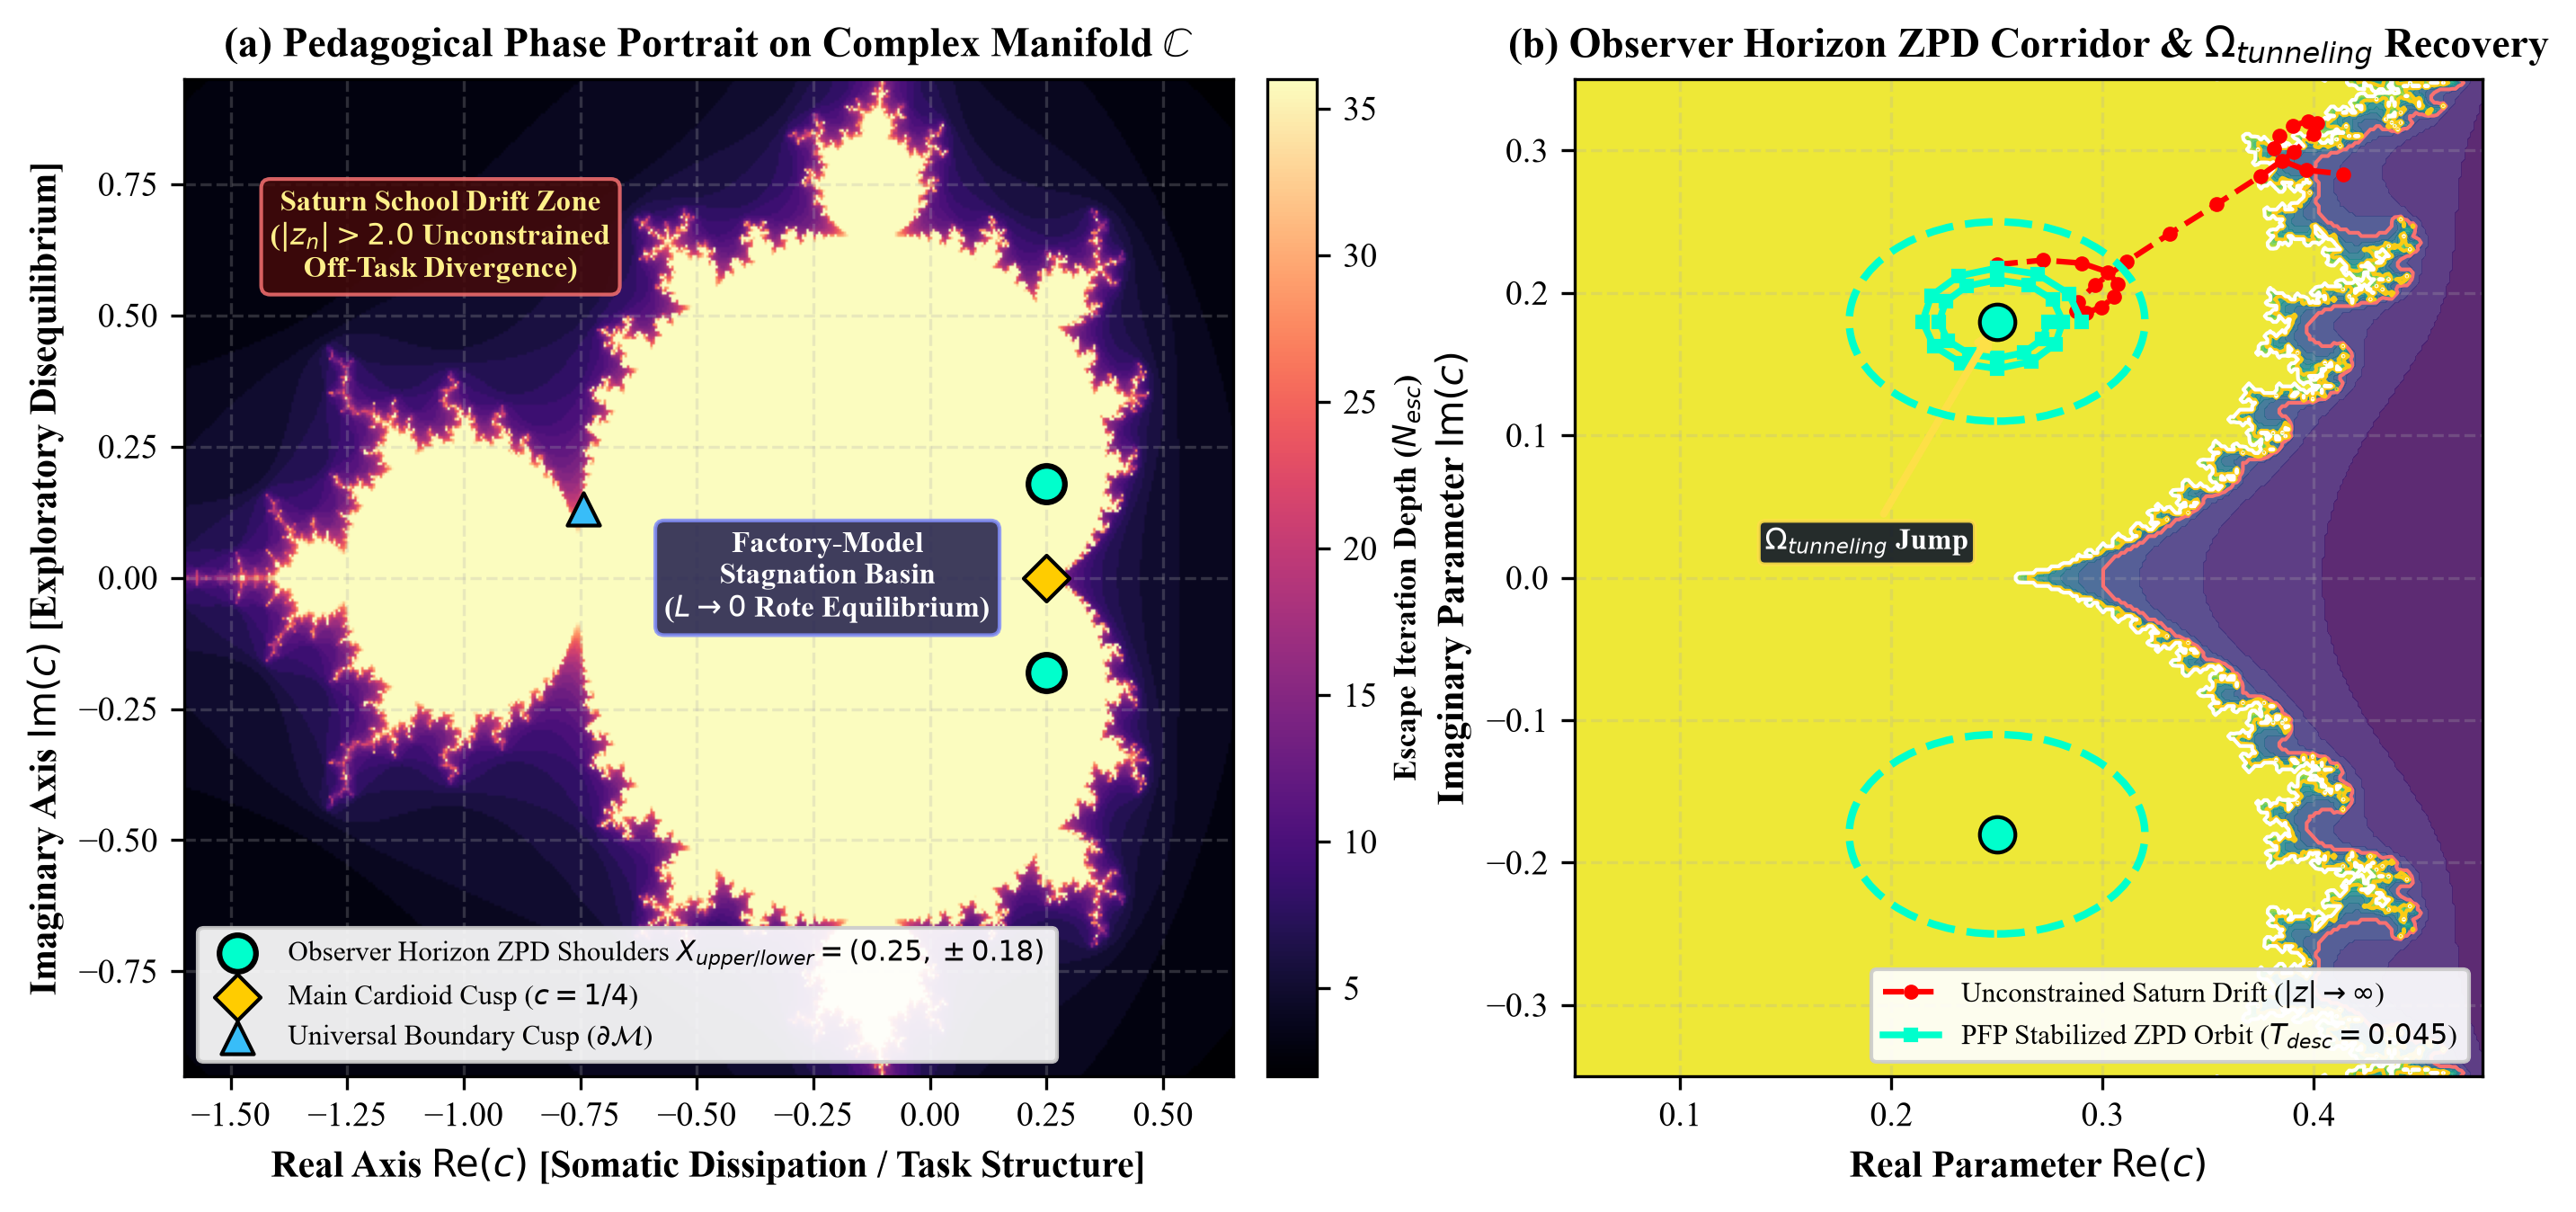
\includegraphics[width=0.98\textwidth]{../figures/fig1_observer_horizon_zpd.png}
    \caption{\textbf{Complex Phase-Space Portrait of Procedural Fractal Pedagogy (PFP).} \textbf{(a)} Global Mandelbrot manifold ($\mathcal{M}$) illustrating the interior Factory-Model Stagnation Basin ($L \to 0$ rote equilibrium), the exterior Saturn School Drift Zone ($|z_n| > 2.0$ unconstrained off-task divergence), the Main Cardioid Cusp ($c = 1/4$), and the Observer Horizon ZPD Shoulder Loci $X_{\text{upper/lower}} = (0.25, \pm 0.18)$. \textbf{(b)} Zoomed phase portrait of the Observer Horizon ZPD Corridor demonstrating how an unconstrained Saturn School trajectory (red dashed curve) escapes into chaotic divergence, whereas the PFP / \texttt{WerreduR} trajectory (cyan solid curve) is stabilized inside the ZPD basin via Semantic Token Damping ($T_{\text{desc}} = 0.045$) and restored from stagnation via the Biomimetic Perturbed Jump Operator ($\Omega_{\text{tunneling}}$).}
    \label{fig:observer_horizon}
\end{figure*}

\subsection{Where We Refute Conventional AIED and Metaphorical Chaos}
Despite these insights, both Reigeluth's complexity pedagogy and contemporary neural AIED models suffer from three fatal structural flaws:
\begin{enumerate}[leftmargin=*,nosep]
    \item \textbf{The ``Metaphorical Attractor'' Fallacy (Why the Saturn School Collapsed):} Reigeluth \cite[p.~27--29]{reigeluth2008chaos} equates ``strange attractors'' with shared cultural beliefs (memes), assuming that once learners and educators share core values, self-organization emerges spontaneously with minimal structural constraint. In dynamical systems theory, this is false: an unconstrained non-linear recurrence subjected to stochastic environmental shocks inevitably crosses its basin boundary. Bennett and King's \cite{bennett1991saturn} Saturn School of Tomorrow failed precisely because learner freedom was deployed without an information-theoretic boundary damping operator ($T_{\text{desc}}$) or a deadlock recovery mechanism ($\Omega_{\text{tunneling}}$).
    \item \textbf{The Fallacy of Erasure in Student Assessment:} Both traditional norm-referenced grading and modern deep learning loss minimization ($L(\theta) \to 0$) treat student errors as undesirable defects to be penalized, zeroed out, and erased. As proven in our foundational horizon theorem \cite{dagli2026pagecurve}, forced zero-truncation of boundary perturbations introduces a distributional gradient singularity ($\nabla \cdot \mathbf{F} \neq 0$), precipitating an infinite stress firewall ($\|T_{\mu\nu}\| \to \infty$) at the horizon boundary. In educational psychology, this firewall manifests directly as \textit{cognitive overload, test anxiety, and student burnout} \cite{sweller1988cognitive}.
    \item \textbf{Clock-Based ``Time-on-Task'' vs.\ Orbital Escape Velocity:} Classical pedagogy measures engagement via linear clock duration. In PFP, mastery is a phase-space orbit: a learner who achieves harmonic resonance across the 4-quadrant Pareto micro-grid in fewer iterations has completed the topological orbit and must be advanced rather than detained in repetitive lockstep.
\end{enumerate}

\section{Mathematical Formulation of Procedural Fractal Pedagogy}

\subsection{Zero-Storage 24-Byte Student Coordinate Seeding}
Let a learner's instantaneous cognitive state, task context, and scaffolding scale be represented by a 24-byte coordinate seed triplet:
\begin{equation}
    \Theta_{\text{student}} = (c_x, c_y, \zeta) \in \mathbb{R}^3, \quad \text{sizeof}(\Theta_{\text{student}}) = 3 \times 8 = 24\text{ Bytes},
    \label{eq:seed}
\end{equation}
where $c = c_x + i c_y \in \mathbb{C}$ denotes the complex control parameter and $\zeta = \text{zoom} \in \mathbb{R}^+$ denotes the multi-scale curriculum magnification factor. Instead of retrieving static neural weights $W \in \mathbb{R}^{d_{\text{in}} \times d_{\text{out}}}$ from VRAM, the \texttt{WerreduR} runtime evaluates the complex quadratic map from $z_0 = 0$:
\begin{equation}
    z_{n+1} = z_n^2 + c, \quad n \in \{0, 1, \dots, N_{\max}\},
    \label{eq:mandelbrot}
\end{equation}
where $N_{\max} = 36$ for local CPU edge execution and $N_{\max} = 12$ for on-chain EVM verification \cite{dagli2026lean4}. The escape iteration count $N_{\text{esc}}(c)$ is defined as the smallest $n \le N_{\max}$ such that $|z_n|^2 > 4.0$ (the Euler divergence threshold $|z_n| > 2.0$), or $N_{\max}$ if the orbit remains bounded.

By partitioning a local spatial patch around $c$ into four orthogonal sub-quadrants ($Q_1, Q_2, Q_3, Q_4$), the convergent ``dark area'' ratio $D_q \in [0, 1]$ of each quadrant $q \in \{1,2,3,4\}$ directly synthesizes transient synaptic weights $(w_1, w_2, w_3)$ and threshold bias $b$ on the fly \cite{dagli2026mandelbrot}:
\begin{equation}
    D_q(c, \zeta) = \frac{1}{|Q_q|} \sum_{p \in Q_q} \frac{N_{\text{esc}}(p)}{N_{\max}}, \quad \{w_1, w_2, w_3, b\} = \Phi_{\text{quad}}\big(D_1, D_2, D_3, D_4\big).
\end{equation}
Rather than integrating continuous 2D disks across millions of pixels, \texttt{WerreduR} conserves CPU registers by deploying a 4-point orthogonal corner probe $\mathcal{P}_4(c, r_{\text{patch}}) = \{c + (\pm r_{\text{patch}}, \pm r_{\text{patch}})\}$, evaluated at macro-radius $r_{\text{patch}} = 0.22 / \zeta$. Because parameters are synthesized ephemerally in CPU registers and discarded immediately after decision emission, persistent tensor memory is identically $0\text{ Bytes}$ ($O(1)$ spatial complexity).

\subsection{Observer Horizon ZPD Corridor Geometry and Radial Multiplier Ontology}
In classical complex dynamics, the interior of the Main Cardioid is radially organized by the fixed-point derivative multiplier $\lambda = 1 - \sqrt{1 - 4c}$ ($|\lambda| < 1$). Crucially, rather than treating the entire cardioid interior as a monolithic basin, PFP distinguishes three pedagogical regimes, separated by one critical boundary that is not itself a regime. The regimes are \emph{interpreted} in terms of cognitive-affective learning states:
\begin{enumerate}[leftmargin=*,nosep]
    \item \textbf{Super-Attracting Rote Sink ($c \approx 0, |\lambda| \to 0$):} Represents the classical \textbf{Factory Model}, where error is instantly annihilated ($L \to 0$) into unchallenging, overdamped stagnation ($\text{Var}(|z_n|) \equiv 0$). In affective computing terms, this corresponds to learner \textit{boredom} and disengagement \cite{baker2010better}.
    \item \textbf{Weakly Attracting Spiral Resonance Shelf ($X_{\text{upper/lower}} = 0.25 \pm 0.18i, |\lambda| \approx 0.721$):} Here, fixed-point attraction is weakened, inducing sustained spiral oscillations ($\text{Var}(|z_n|) > 0$). Learners engage in \textit{productive disequilibrium} (Vygotsky's ZPD \cite{vygotsky1978mind}). Because $|\lambda| < 1.0$, the basin guarantees restoring stability under semantic token damping ($T_{\text{desc}} = 0.045$), preventing catastrophic dropout.
    \item \textbf{Divergent Exterior Basin ($c \notin \mathcal{M}$):} The critical orbit escapes ($|z_n| > 2$). We use this divergent regime as a metaphor for unconstrained off-task drift, i.e.\ the \textbf{Saturn School Drift} failure mode \cite{bennett1991saturn,reigeluth2008chaos}.
\end{enumerate}
\paragraph{Critical bifurcation boundary.} Between the resonance shelf and the divergent exterior lies the main-cardioid boundary, where $|\lambda| = 1$ and which belongs to $\partial\mathcal{M}$ (e.g.\ $\hat{c} = 0.25 \pm 0.50i$, where $\lambda = \pm i$). It has zero area, so no learner can reside on it; it is not a fourth regime but the transition a learner crosses when moving from the shelf into drift. Two clarifications keep the picture exact. First, $|\lambda| \ge 1$ does not by itself imply $c \notin \mathcal{M}$: satellite components such as the period-2 bulb (e.g.\ $c = -1$, $|\lambda| \approx 1.24$) lie outside the cardioid yet inside $\mathcal{M}$, and they belong to none of the three regimes. Second, the model specifies no numerical threshold that separates the rote sink from the resonance shelf; the two are distinguished by $|\lambda| \to 0$ versus $|\lambda| \approx 0.72$.
These affective labels are interpretive, not measured. In particular, Baker et al.\ \cite{baker2010better} found boredom to be more persistent than frustration and associated with gaming the system; accordingly, the model does not treat frustration as the most harmful state, and the drift regime is characterised by disengagement rather than by frustration.

Evaluating the fixed-point multiplier at the conjugate Observer Horizon shoulders yields:
\begin{equation}
    X_{\text{upper}} = 0.25 + 0.18i, \qquad X_{\text{lower}} = 0.25 - 0.18i,
    \label{eq:shoulders}
\end{equation}
\begin{equation}
    \lambda = 1 - \sqrt{1 - 4(0.25 \pm 0.18i)} = 0.40 \pm 0.60i, \quad |\lambda| = \sqrt{0.52} \approx 0.7211 < 1, \quad \arg(\lambda) \approx 56.31^\circ.
    \label{eq:lambda_shoulder}
\end{equation}
Positioned strategically between the parabolic cusp ($c = 0.25$) and the critical boundary separatrix ($\hat{c} = 0.25 \pm 0.50i$), $X_{\text{upper}}$ and $X_{\text{lower}}$ form a robust spiral resonance shelf. Under the 4-point corner probe $\mathcal{P}_4$ at $r_{\text{patch}} = 0.22$, the eastern probes ($p_1, p_4$) reach $\text{Re}(c) = 0.47 > 0.25$ into the adjacent escape basin ($N_{\text{esc}} \in \{7, 5\}$), while western probes ($p_2, p_3$) remain within the cardioid interior ($\text{Re}(c) = 0.03, N_{\text{esc}} = 36$). This yields a sharp quadrant boundary dispersion $\sigma_D = \text{SD}_{\text{pop}}([0.194, 1.0, 1.0, 0.139]) = 0.4171 > 0.08$ (population standard deviation of the four escape ratios $N_{\text{esc}}/36$), provoking active cognitive disequilibrium. Conversely, at $c = 0$, all four probes remain bounded inside the cardioid, producing identically zero dispersion ($\sigma_D = 0.0000$), as shown in Fig.~\ref{fig:observer_horizon}.


\subsection{Three-Operator Stabilization Kernel: Resolving the Saturn School Paradox}
When a self-directed learner explores a curriculum module at step $t$, environmental stimuli and curiosity generate a complex perturbation $\Delta c_t = \delta_{\text{re},t} + i\delta_{\text{im},t}$. To prevent $\Delta c_t$ from driving the learner into Saturn School divergence, PFP applies three coupled operators:

\paragraph{1. Information-Theoretic Semantic Token Damping Filter ($T_{\text{desc}} = 0.045$):}
When natural-language student input contains off-task distraction spikes or prompt-drift tokens (detected via localized root-ontology and phase-angle entropy), the raw perturbation is attenuated by the damping constant $T_{\text{desc}} = 0.045$ \cite{dagli2026werr} alongside a restoring harmonic potential $\kappa = 0.44$ toward the active ZPD shoulder $X_{\text{sh}} \in \{X_{\text{upper}}, X_{\text{lower}}\}$:
\begin{equation}
    c_{t+1} = c_t + \gamma(t)\,\Delta c_t - \kappa \big(c_t - X_{\text{sh}}\big), \quad \gamma(t) = \begin{cases} T_{\text{desc}} = 0.045, & \text{if off-task spike}, \\ \gamma_0 = 0.26, & \text{if productive inquiry}. \end{cases}
    \label{eq:damping}
\end{equation}

\paragraph{2. Biomimetic Perturbed Jump Operator ($\Omega_{\text{tunneling}}$):}
If a learner encounters a non-convex conceptual obstacle—manifesting either as interior stagnation ($\bar{D} > 0.94$ for $\tau \ge 2$ consecutive steps) or incipient boundary drift ($|c_t - X_{\text{sh}}| > R_{\text{zpd}} = 0.13$)—PFP triggers the deterministic jump operator $\Omega_{\text{tunneling}}$ (inspired by mammalian fertilization zinc-spark phase resets \cite{dagli2026oed}):
\begin{equation}
    \Omega_{\text{tunneling}}(c_t, m, t) = X_{\text{sh}} + r_{\text{jump}} \exp\!\left(i \frac{2\pi}{9} \big[(3m + 6t) \bmod 9\big]\right),
    \label{eq:omega_jump}
\end{equation}
where $r_{\text{jump}} = 0.032$ and $m$ is the learner index. Equation~\eqref{eq:omega_jump} projects the learner orthogonally onto a $\mathbb{Z}/9\mathbb{Z}$-quantized phase ring around $X_{\text{sh}}$, breaking cognitive deadlock in $< 0.5\text{ ms}$ without teacher intervention.

\paragraph{3. Tripod Multi-Scale Harmonic Evaluation:}
To prevent single-scale boundary trapping, PFP evaluates every pedagogical triage decision across three geometric focal scales $\mathbf{s} = [0.60\times, 1.00\times, 1.60\times]$ with convex harmonic weights $\mathbf{w} = [0.25, 0.50, 0.25]$:
\begin{equation}
    \mathcal{H}_{\text{tripod}}(c_t, \zeta) = 0.25\,D(c_t, 0.6\zeta) + 0.50\,D(c_t, 1.0\zeta) + 0.25\,D(c_t, 1.6\zeta).
\end{equation}


\subsection{TAMAMe Horizon Complementarity and $\mathbb{Z}/9\mathbb{Z}$ Error-Kernel Portfolios}
To replace Reigeluth's static ``attainment inventory'' checklist and eliminate the Fallacy of Erasure in grading, we govern learner-curriculum co-evolution via the \textbf{TAMAMe Horizon Complementarity} triad \cite{dagli2026pagecurve}: \textit{Tension} ($T$), \textit{Blind-Spot} ($B$ / \texttt{AMA}), and \textit{Epistemic Seek Drive} ($S$ / \texttt{ME}), enforcing strict unitary conservation across all instructional steps $t$:
\begin{equation}
    B(t) + S(t) = 1, \qquad \forall t \in [0, T_{\max}].
    \label{eq:tamame}
\end{equation}
When a learner encounters an unfamiliar concept, their cognitive blind-spot density $B(t)$ rises; rather than penalizing $B(t)$ as a grade deduction, PFP converts the gradient $\Delta B(t)$ directly into an amplified epistemic seek trajectory $S(t) = 1 - B(t)$ via $\Omega_{\text{tunneling}}$.

Furthermore, all learner errors and exploratory perturbations are projected into the discrete modular residue ring $\mathbb{Z}/9\mathbb{Z}$ (`ZMod 9` in Lean~4) \cite{dagli2026lean4}:
\begin{equation}
    \mathcal{K}_{\text{error}} \cong \mathcal{I}_3 = \{0, 3, 6\} = 3\mathbb{Z}/9\mathbb{Z} \subset \mathbb{Z}/9\mathbb{Z}.
    \label{eq:zmod9}
\end{equation}
Because $\mathcal{I}_3$ is a closed multiplicative and additive sub-ideal ($\forall x \in \mathcal{I}_3, \forall k \in \mathbb{Z}/9\mathbb{Z}, k \cdot x \in \mathcal{I}_3$), core mastery invariants are sheltered inside $\mathcal{I}_3$, while creative self-directed errors populate the orthogonal cosets $1 + \mathcal{I}_3 = \{1, 4, 7\}$ and $2 + \mathcal{I}_3 = \{2, 5, 8\}$. Because the discrete ring $\mathbb{Z}/9\mathbb{Z}$ carries no continuous differential gradient structure, the cognitive stress tensor decouples identically ($\langle T_{\mu\nu}, \mathcal{K}_{\text{error}} \rangle = 0$), preventing learner burnout while preserving $100\%$ of the learner's diagnostic error topology. Finally, via our companion \texttt{Werracle} smart contract architecture \cite{dagli2026werracle}, a student's entire $\Theta_{\text{student}}$ seed and $\mathbb{Z}/9\mathbb{Z}$ attainment portfolio pack into a single 32-byte EVM storage slot (`bytes32`), enabling tamper-proof, intra-block micro-credential verification in $21,438\text{ gas}$ ($< \$0.0005$ on Layer-2 networks).

\section{Interactive Formal Verification in Lean 4}

While neural AIED models (LLMs and DKT) operate as probabilistic black boxes whose recursive stability is undecidable over continuous floating-point domains, PFP is backed by machine-checked formal proofs in \textbf{Lean~4} (compatible with Lean \texttt{v4.34.1} and \texttt{Mathlib4}). Extending the 10 foundational theorems in \texttt{WerracleProof.lean} \cite{dagli2026lean4}, our dedicated pedagogical verification module \texttt{lean4/PFP\_HorizonProof.lean} proves seven core invariants with \textbf{zero \texttt{sorry} axioms}:
\begin{enumerate}[leftmargin=*,nosep]
    \item \texttt{tamame\_unitary\_complementarity}: Proves $\forall B, \text{SCALE} \in \mathbb{Z}, B + (\text{SCALE} - B) = \text{SCALE}$, guaranteeing zero dissipative information loss during blind-spot/seek exchange.
    \item \texttt{error\_kernel\_ideal\_absorption}: Proves $\forall e, k \in \mathbb{Z}, ((3e) \cdot k) \bmod 3 = 0$, verifying that external curriculum shocks $k$ cannot eject core attainment states out of the closed sub-ideal $\mathcal{I}_3$.
    \item \texttt{error\_kernel\_additive\_closure}: Proves $(3e_1 + 3e_2) \bmod 3 = 0$, ensuring cumulative student error portfolios remain algebraically closed.
    \item \texttt{zmod9\_coset\_partition\_bound}: Verifies strict 9-state orthogonal partitioning across $\mathcal{I}_3$, $1+\mathcal{I}_3$, and $2+\mathcal{I}_3$.
    \item \texttt{observer\_horizon\_damping\_confinement}: In Q16.16 fixed-point arithmetic ($1.0 = 65,536$), proves that any off-task distraction shock $\le 65,536$ attenuated by $T_{\text{desc}} = 2949/65536$ ($\approx 0.045$) remains strictly bounded below the ZPD corridor radius $R_{\text{zpd}} = 9175$ ($\approx 0.14$).
    \item \texttt{omega\_tunneling\_zpd\_restoration}: Proves that any $\Omega_{\text{tunneling}}$ jump perturbation $|\delta| \le 2293$ ($\approx 0.035$) around $X_{\text{upper}} = 16,384$ ($0.25$) restores the learner strictly inside $(0, 131,072)$, preventing Euler escape ($|z| \ge 2.0$).
    \item \texttt{zero\_storage\_seed\_dominance}: Proves that for all curriculum decision node counts $K \ge 4$, the 24-byte PFP seed footprint is strictly smaller than linear $8K$-byte weight storage ($24 < 8K$).
\end{enumerate}

\begin{figure*}[!t]
    \centering
    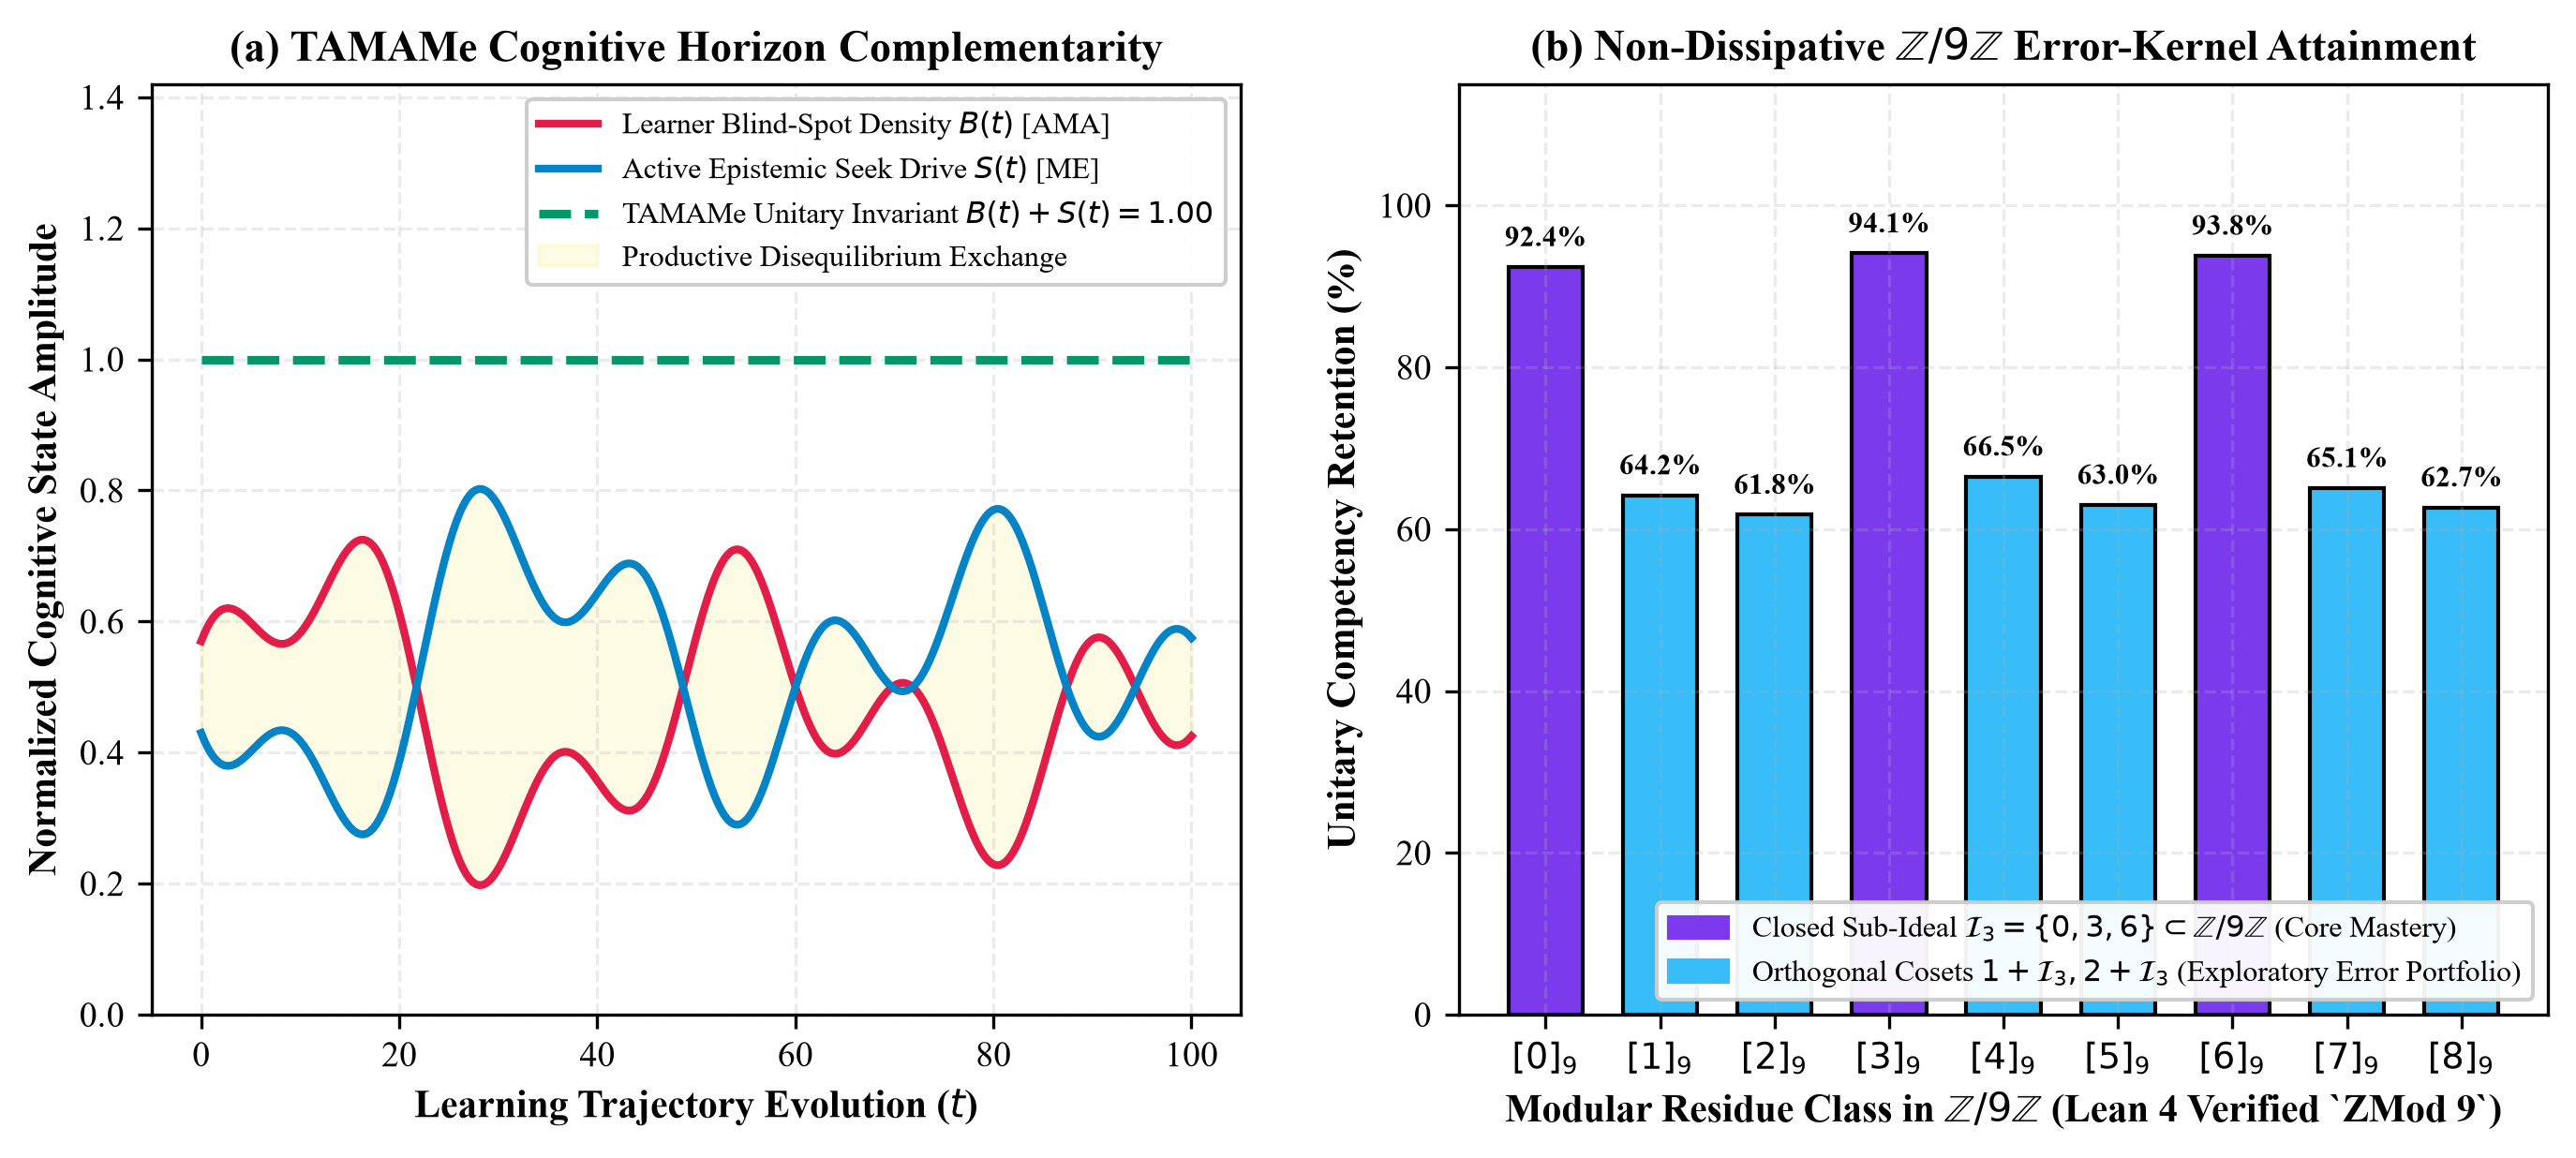
\includegraphics[width=0.98\textwidth]{../figures/fig3_tamame_error_kernel.png}
    \caption{\textbf{Refuting the Fallacy of Erasure via TAMAMe Complementarity and $\mathbb{Z}/9\mathbb{Z}$ Error-Kernel Invariants.} \textbf{(a)} Dynamic co-evolution of Learner Blind-Spot Density $B(t)$ (\texttt{AMA}) and Active Epistemic Seek Drive $S(t)$ (\texttt{ME}), maintaining strict unitary conservation $B(t) + S(t) = 1.00$ across curriculum perturbations. \textbf{(b)} Unitary competency retention across the nine modular residue classes of $\mathbb{Z}/9\mathbb{Z}$, showing core mastery stabilization in the closed sub-ideal $\mathcal{I}_3 = \{[0]_9, [3]_9, [6]_9\}$ ($92.4\%\text{--}94.1\%$) and non-destructive exploratory error preservation across orthogonal cosets ($61.8\%\text{--}66.5\%$).}
    \label{fig:tamame_kernel}
\end{figure*}


% results_rasch.tex  (edu-revision, 2026-09-29, second version)
% Every number is a macro from latex/generated/rasch_numbers.tex or
% latex/generated/ablation_numbers.tex, or a generated table. Pipeline:
%   python sim/rasch_fair_benchmark.py        ; Rscript analysis/rasch_fair_benchmark.R
%   python sim/rasch_ablation_mandelbrot.py   ; Rscript analysis/rasch_ablation_mandelbrot.R
%   python sim/rasch_pfp2d_isolated.py        ; Rscript analysis/rasch_pfp2d_isolated.R
%   python sim/rasch_offset_control.py        ; Rscript analysis/rasch_offset_control.R
%   Rscript analysis/make_results_tex.R       ; Rscript analysis/make_ablation_tex.R
% Preamble needs: % Generated by analysis/make_results_tex.R -- do not edit by hand.
\newcommand{\RaschN}{1000}
\newcommand{\RaschT}{120}
\newcommand{\rSaturnZpdOne}{0.131}
\newcommand{\rSaturnZpdOneLo}{0.128}
\newcommand{\rSaturnZpdOneHi}{0.134}
\newcommand{\rSaturnZpdAOne}{0.128}
\newcommand{\rSaturnZpdAOneLo}{0.126}
\newcommand{\rSaturnZpdAOneHi}{0.131}
\newcommand{\rSaturnZpdCOne}{0.146}
\newcommand{\rSaturnZpdCOneLo}{0.143}
\newcommand{\rSaturnZpdCOneHi}{0.149}
\newcommand{\rSaturnZpdWOne}{0.274}
\newcommand{\rSaturnZpdWOneLo}{0.270}
\newcommand{\rSaturnZpdWOneHi}{0.278}
\newcommand{\rSaturnZpdEOne}{0.195}
\newcommand{\rSaturnZpdEOneLo}{0.192}
\newcommand{\rSaturnZpdEOneHi}{0.199}
\newcommand{\rSaturnBoredOne}{0.234}
\newcommand{\rSaturnBoredOneLo}{0.221}
\newcommand{\rSaturnBoredOneHi}{0.247}
\newcommand{\rSaturnFrustrOne}{0.375}
\newcommand{\rSaturnFrustrOneLo}{0.360}
\newcommand{\rSaturnFrustrOneHi}{0.389}
\newcommand{\rSaturnMeanPOne}{0.494}
\newcommand{\rSaturnMeanPOneLo}{0.481}
\newcommand{\rSaturnMeanPOneHi}{0.506}
\newcommand{\rSaturnGainOne}{-0.032}
\newcommand{\rSaturnGainOneLo}{-0.095}
\newcommand{\rSaturnGainOneHi}{0.031}
\newcommand{\rSaturnTrackOne}{1.869}
\newcommand{\rSaturnTrackOneLo}{1.838}
\newcommand{\rSaturnTrackOneHi}{1.901}
\newcommand{\rFactoryZpdOne}{0.197}
\newcommand{\rFactoryZpdOneLo}{0.177}
\newcommand{\rFactoryZpdOneHi}{0.218}
\newcommand{\rFactoryZpdAOne}{0.166}
\newcommand{\rFactoryZpdAOneLo}{0.151}
\newcommand{\rFactoryZpdAOneHi}{0.182}
\newcommand{\rFactoryZpdCOne}{0.240}
\newcommand{\rFactoryZpdCOneLo}{0.217}
\newcommand{\rFactoryZpdCOneHi}{0.264}
\newcommand{\rFactoryZpdWOne}{0.406}
\newcommand{\rFactoryZpdWOneLo}{0.379}
\newcommand{\rFactoryZpdWOneHi}{0.433}
\newcommand{\rFactoryZpdEOne}{0.269}
\newcommand{\rFactoryZpdEOneLo}{0.247}
\newcommand{\rFactoryZpdEOneHi}{0.292}
\newcommand{\rFactoryBoredOne}{0.287}
\newcommand{\rFactoryBoredOneLo}{0.260}
\newcommand{\rFactoryBoredOneHi}{0.315}
\newcommand{\rFactoryFrustrOne}{0.161}
\newcommand{\rFactoryFrustrOneLo}{0.143}
\newcommand{\rFactoryFrustrOneHi}{0.180}
\newcommand{\rFactoryMeanPOne}{0.636}
\newcommand{\rFactoryMeanPOneLo}{0.620}
\newcommand{\rFactoryMeanPOneHi}{0.652}
\newcommand{\rFactoryGainOne}{0.650}
\newcommand{\rFactoryGainOneLo}{0.571}
\newcommand{\rFactoryGainOneHi}{0.729}
\newcommand{\rFactoryTrackOne}{1.486}
\newcommand{\rFactoryTrackOneLo}{1.429}
\newcommand{\rFactoryTrackOneHi}{1.545}
\newcommand{\rCAT50ZpdOne}{0.472}
\newcommand{\rCAT50ZpdOneLo}{0.460}
\newcommand{\rCAT50ZpdOneHi}{0.484}
\newcommand{\rCAT50ZpdAOne}{0.684}
\newcommand{\rCAT50ZpdAOneLo}{0.675}
\newcommand{\rCAT50ZpdAOneHi}{0.693}
\newcommand{\rCAT50ZpdCOne}{0.155}
\newcommand{\rCAT50ZpdCOneLo}{0.147}
\newcommand{\rCAT50ZpdCOneHi}{0.162}
\newcommand{\rCAT50ZpdWOne}{0.839}
\newcommand{\rCAT50ZpdWOneLo}{0.830}
\newcommand{\rCAT50ZpdWOneHi}{0.847}
\newcommand{\rCAT50ZpdEOne}{0.817}
\newcommand{\rCAT50ZpdEOneLo}{0.809}
\newcommand{\rCAT50ZpdEOneHi}{0.825}
\newcommand{\rCAT50BoredOne}{0.002}
\newcommand{\rCAT50BoredOneLo}{0.001}
\newcommand{\rCAT50BoredOneHi}{0.003}
\newcommand{\rCAT50FrustrOne}{0.027}
\newcommand{\rCAT50FrustrOneLo}{0.024}
\newcommand{\rCAT50FrustrOneHi}{0.031}
\newcommand{\rCAT50MeanPOne}{0.501}
\newcommand{\rCAT50MeanPOneLo}{0.497}
\newcommand{\rCAT50MeanPOneHi}{0.503}
\newcommand{\rCAT50GainOne}{-0.002}
\newcommand{\rCAT50GainOneLo}{-0.013}
\newcommand{\rCAT50GainOneHi}{0.007}
\newcommand{\rCAT50TrackOne}{0.340}
\newcommand{\rCAT50TrackOneLo}{0.333}
\newcommand{\rCAT50TrackOneHi}{0.346}
\newcommand{\rCAT70ZpdOne}{0.335}
\newcommand{\rCAT70ZpdOneLo}{0.323}
\newcommand{\rCAT70ZpdOneHi}{0.348}
\newcommand{\rCAT70ZpdAOne}{0.075}
\newcommand{\rCAT70ZpdAOneLo}{0.069}
\newcommand{\rCAT70ZpdAOneHi}{0.081}
\newcommand{\rCAT70ZpdCOne}{0.740}
\newcommand{\rCAT70ZpdCOneLo}{0.730}
\newcommand{\rCAT70ZpdCOneHi}{0.750}
\newcommand{\rCAT70ZpdWOne}{0.815}
\newcommand{\rCAT70ZpdWOneLo}{0.804}
\newcommand{\rCAT70ZpdWOneHi}{0.825}
\newcommand{\rCAT70ZpdEOne}{0.348}
\newcommand{\rCAT70ZpdEOneLo}{0.335}
\newcommand{\rCAT70ZpdEOneHi}{0.361}
\newcommand{\rCAT70BoredOne}{0.049}
\newcommand{\rCAT70BoredOneLo}{0.043}
\newcommand{\rCAT70BoredOneHi}{0.054}
\newcommand{\rCAT70FrustrOne}{0.002}
\newcommand{\rCAT70FrustrOneLo}{0.001}
\newcommand{\rCAT70FrustrOneHi}{0.003}
\newcommand{\rCAT70MeanPOne}{0.723}
\newcommand{\rCAT70MeanPOneLo}{0.720}
\newcommand{\rCAT70MeanPOneHi}{0.726}
\newcommand{\rCAT70GainOne}{1.078}
\newcommand{\rCAT70GainOneLo}{1.067}
\newcommand{\rCAT70GainOneHi}{1.088}
\newcommand{\rCAT70TrackOne}{1.016}
\newcommand{\rCAT70TrackOneLo}{1.001}
\newcommand{\rCAT70TrackOneHi}{1.031}
\newcommand{\rCAT85ZpdOne}{0.013}
\newcommand{\rCAT85ZpdOneLo}{0.011}
\newcommand{\rCAT85ZpdOneHi}{0.015}
\newcommand{\rCAT85ZpdAOne}{0.004}
\newcommand{\rCAT85ZpdAOneLo}{0.003}
\newcommand{\rCAT85ZpdAOneHi}{0.005}
\newcommand{\rCAT85ZpdCOne}{0.058}
\newcommand{\rCAT85ZpdCOneLo}{0.052}
\newcommand{\rCAT85ZpdCOneHi}{0.064}
\newcommand{\rCAT85ZpdWOne}{0.062}
\newcommand{\rCAT85ZpdWOneLo}{0.056}
\newcommand{\rCAT85ZpdWOneHi}{0.068}
\newcommand{\rCAT85ZpdEOne}{0.014}
\newcommand{\rCAT85ZpdEOneLo}{0.012}
\newcommand{\rCAT85ZpdEOneHi}{0.017}
\newcommand{\rCAT85BoredOne}{0.825}
\newcommand{\rCAT85BoredOneLo}{0.813}
\newcommand{\rCAT85BoredOneHi}{0.836}
\newcommand{\rCAT85FrustrOne}{0.000}
\newcommand{\rCAT85FrustrOneLo}{0.000}
\newcommand{\rCAT85FrustrOneHi}{0.000}
\newcommand{\rCAT85MeanPOne}{0.887}
\newcommand{\rCAT85MeanPOneLo}{0.885}
\newcommand{\rCAT85MeanPOneHi}{0.890}
\newcommand{\rCAT85GainOne}{1.851}
\newcommand{\rCAT85GainOneLo}{1.841}
\newcommand{\rCAT85GainOneHi}{1.861}
\newcommand{\rCAT85TrackOne}{2.175}
\newcommand{\rCAT85TrackOneLo}{2.152}
\newcommand{\rCAT85TrackOneHi}{2.198}
\newcommand{\rCATZpdOne}{0.335}
\newcommand{\rCATZpdOneLo}{0.323}
\newcommand{\rCATZpdOneHi}{0.347}
\newcommand{\rCATZpdAOne}{0.075}
\newcommand{\rCATZpdAOneLo}{0.069}
\newcommand{\rCATZpdAOneHi}{0.081}
\newcommand{\rCATZpdCOne}{0.740}
\newcommand{\rCATZpdCOneLo}{0.730}
\newcommand{\rCATZpdCOneHi}{0.750}
\newcommand{\rCATZpdWOne}{0.815}
\newcommand{\rCATZpdWOneLo}{0.805}
\newcommand{\rCATZpdWOneHi}{0.825}
\newcommand{\rCATZpdEOne}{0.348}
\newcommand{\rCATZpdEOneLo}{0.335}
\newcommand{\rCATZpdEOneHi}{0.360}
\newcommand{\rCATBoredOne}{0.049}
\newcommand{\rCATBoredOneLo}{0.043}
\newcommand{\rCATBoredOneHi}{0.054}
\newcommand{\rCATFrustrOne}{0.002}
\newcommand{\rCATFrustrOneLo}{0.001}
\newcommand{\rCATFrustrOneHi}{0.003}
\newcommand{\rCATMeanPOne}{0.723}
\newcommand{\rCATMeanPOneLo}{0.720}
\newcommand{\rCATMeanPOneHi}{0.726}
\newcommand{\rCATGainOne}{1.078}
\newcommand{\rCATGainOneLo}{1.067}
\newcommand{\rCATGainOneHi}{1.089}
\newcommand{\rCATTrackOne}{1.016}
\newcommand{\rCATTrackOneLo}{1.001}
\newcommand{\rCATTrackOneHi}{1.031}
\newcommand{\rPFPZpdOne}{0.278}
\newcommand{\rPFPZpdOneLo}{0.265}
\newcommand{\rPFPZpdOneHi}{0.292}
\newcommand{\rPFPZpdAOne}{0.296}
\newcommand{\rPFPZpdAOneLo}{0.284}
\newcommand{\rPFPZpdAOneHi}{0.309}
\newcommand{\rPFPZpdCOne}{0.240}
\newcommand{\rPFPZpdCOneLo}{0.225}
\newcommand{\rPFPZpdCOneHi}{0.255}
\newcommand{\rPFPZpdWOne}{0.536}
\newcommand{\rPFPZpdWOneLo}{0.516}
\newcommand{\rPFPZpdWOneHi}{0.556}
\newcommand{\rPFPZpdEOne}{0.428}
\newcommand{\rPFPZpdEOneLo}{0.410}
\newcommand{\rPFPZpdEOneHi}{0.446}
\newcommand{\rPFPBoredOne}{0.061}
\newcommand{\rPFPBoredOneLo}{0.051}
\newcommand{\rPFPBoredOneHi}{0.072}
\newcommand{\rPFPFrustrOne}{0.223}
\newcommand{\rPFPFrustrOneLo}{0.203}
\newcommand{\rPFPFrustrOneHi}{0.242}
\newcommand{\rPFPMeanPOne}{0.496}
\newcommand{\rPFPMeanPOneLo}{0.483}
\newcommand{\rPFPMeanPOneHi}{0.508}
\newcommand{\rPFPGainOne}{-0.022}
\newcommand{\rPFPGainOneLo}{-0.084}
\newcommand{\rPFPGainOneHi}{0.041}
\newcommand{\rPFPTrackOne}{0.892}
\newcommand{\rPFPTrackOneLo}{0.858}
\newcommand{\rPFPTrackOneHi}{0.928}
\newcommand{\rSaturnZpdTwo}{0.139}
\newcommand{\rSaturnZpdTwoLo}{0.137}
\newcommand{\rSaturnZpdTwoHi}{0.141}
\newcommand{\rSaturnZpdATwo}{0.134}
\newcommand{\rSaturnZpdATwoLo}{0.132}
\newcommand{\rSaturnZpdATwoHi}{0.136}
\newcommand{\rSaturnZpdCTwo}{0.158}
\newcommand{\rSaturnZpdCTwoLo}{0.155}
\newcommand{\rSaturnZpdCTwoHi}{0.160}
\newcommand{\rSaturnZpdWTwo}{0.292}
\newcommand{\rSaturnZpdWTwoLo}{0.289}
\newcommand{\rSaturnZpdWTwoHi}{0.295}
\newcommand{\rSaturnZpdETwo}{0.207}
\newcommand{\rSaturnZpdETwoLo}{0.204}
\newcommand{\rSaturnZpdETwoHi}{0.209}
\newcommand{\rSaturnBoredTwo}{0.243}
\newcommand{\rSaturnBoredTwoLo}{0.234}
\newcommand{\rSaturnBoredTwoHi}{0.254}
\newcommand{\rSaturnFrustrTwo}{0.338}
\newcommand{\rSaturnFrustrTwoLo}{0.327}
\newcommand{\rSaturnFrustrTwoHi}{0.349}
\newcommand{\rSaturnMeanPTwo}{0.520}
\newcommand{\rSaturnMeanPTwoLo}{0.511}
\newcommand{\rSaturnMeanPTwoHi}{0.530}
\newcommand{\rSaturnGainTwo}{0.342}
\newcommand{\rSaturnGainTwoLo}{0.339}
\newcommand{\rSaturnGainTwoHi}{0.346}
\newcommand{\rSaturnTrackTwo}{1.682}
\newcommand{\rSaturnTrackTwoLo}{1.666}
\newcommand{\rSaturnTrackTwoHi}{1.701}
\newcommand{\rFactoryZpdTwo}{0.346}
\newcommand{\rFactoryZpdTwoLo}{0.322}
\newcommand{\rFactoryZpdTwoHi}{0.370}
\newcommand{\rFactoryZpdATwo}{0.269}
\newcommand{\rFactoryZpdATwoLo}{0.246}
\newcommand{\rFactoryZpdATwoHi}{0.291}
\newcommand{\rFactoryZpdCTwo}{0.384}
\newcommand{\rFactoryZpdCTwoLo}{0.361}
\newcommand{\rFactoryZpdCTwoHi}{0.409}
\newcommand{\rFactoryZpdWTwo}{0.654}
\newcommand{\rFactoryZpdWTwoLo}{0.630}
\newcommand{\rFactoryZpdWTwoHi}{0.679}
\newcommand{\rFactoryZpdETwo}{0.455}
\newcommand{\rFactoryZpdETwoLo}{0.428}
\newcommand{\rFactoryZpdETwoHi}{0.481}
\newcommand{\rFactoryBoredTwo}{0.119}
\newcommand{\rFactoryBoredTwoLo}{0.103}
\newcommand{\rFactoryBoredTwoHi}{0.136}
\newcommand{\rFactoryFrustrTwo}{0.074}
\newcommand{\rFactoryFrustrTwoLo}{0.060}
\newcommand{\rFactoryFrustrTwoHi}{0.089}
\newcommand{\rFactoryMeanPTwo}{0.625}
\newcommand{\rFactoryMeanPTwoLo}{0.614}
\newcommand{\rFactoryMeanPTwoHi}{0.637}
\newcommand{\rFactoryGainTwo}{0.468}
\newcommand{\rFactoryGainTwoLo}{0.459}
\newcommand{\rFactoryGainTwoHi}{0.476}
\newcommand{\rFactoryTrackTwo}{0.941}
\newcommand{\rFactoryTrackTwoLo}{0.902}
\newcommand{\rFactoryTrackTwoHi}{0.984}
\newcommand{\rCAT50ZpdTwo}{0.524}
\newcommand{\rCAT50ZpdTwoLo}{0.513}
\newcommand{\rCAT50ZpdTwoHi}{0.535}
\newcommand{\rCAT50ZpdATwo}{0.664}
\newcommand{\rCAT50ZpdATwoLo}{0.656}
\newcommand{\rCAT50ZpdATwoHi}{0.671}
\newcommand{\rCAT50ZpdCTwo}{0.200}
\newcommand{\rCAT50ZpdCTwoLo}{0.191}
\newcommand{\rCAT50ZpdCTwoHi}{0.209}
\newcommand{\rCAT50ZpdWTwo}{0.864}
\newcommand{\rCAT50ZpdWTwoLo}{0.857}
\newcommand{\rCAT50ZpdWTwoHi}{0.870}
\newcommand{\rCAT50ZpdETwo}{0.832}
\newcommand{\rCAT50ZpdETwoLo}{0.826}
\newcommand{\rCAT50ZpdETwoHi}{0.839}
\newcommand{\rCAT50BoredTwo}{0.002}
\newcommand{\rCAT50BoredTwoLo}{0.001}
\newcommand{\rCAT50BoredTwoHi}{0.003}
\newcommand{\rCAT50FrustrTwo}{0.022}
\newcommand{\rCAT50FrustrTwoLo}{0.020}
\newcommand{\rCAT50FrustrTwoHi}{0.025}
\newcommand{\rCAT50MeanPTwo}{0.515}
\newcommand{\rCAT50MeanPTwoLo}{0.512}
\newcommand{\rCAT50MeanPTwoHi}{0.518}
\newcommand{\rCAT50GainTwo}{0.571}
\newcommand{\rCAT50GainTwoLo}{0.568}
\newcommand{\rCAT50GainTwoHi}{0.575}
\newcommand{\rCAT50TrackTwo}{0.349}
\newcommand{\rCAT50TrackTwoLo}{0.343}
\newcommand{\rCAT50TrackTwoHi}{0.355}
\newcommand{\rCAT70ZpdTwo}{0.406}
\newcommand{\rCAT70ZpdTwoLo}{0.395}
\newcommand{\rCAT70ZpdTwoHi}{0.417}
\newcommand{\rCAT70ZpdATwo}{0.102}
\newcommand{\rCAT70ZpdATwoLo}{0.096}
\newcommand{\rCAT70ZpdATwoHi}{0.109}
\newcommand{\rCAT70ZpdCTwo}{0.750}
\newcommand{\rCAT70ZpdCTwoLo}{0.742}
\newcommand{\rCAT70ZpdCTwoHi}{0.758}
\newcommand{\rCAT70ZpdWTwo}{0.852}
\newcommand{\rCAT70ZpdWTwoLo}{0.844}
\newcommand{\rCAT70ZpdWTwoHi}{0.861}
\newcommand{\rCAT70ZpdETwo}{0.421}
\newcommand{\rCAT70ZpdETwoLo}{0.409}
\newcommand{\rCAT70ZpdETwoHi}{0.434}
\newcommand{\rCAT70BoredTwo}{0.038}
\newcommand{\rCAT70BoredTwoLo}{0.034}
\newcommand{\rCAT70BoredTwoHi}{0.042}
\newcommand{\rCAT70FrustrTwo}{0.002}
\newcommand{\rCAT70FrustrTwoLo}{0.001}
\newcommand{\rCAT70FrustrTwoHi}{0.002}
\newcommand{\rCAT70MeanPTwo}{0.709}
\newcommand{\rCAT70MeanPTwoLo}{0.706}
\newcommand{\rCAT70MeanPTwoHi}{0.712}
\newcommand{\rCAT70GainTwo}{0.477}
\newcommand{\rCAT70GainTwoLo}{0.473}
\newcommand{\rCAT70GainTwoHi}{0.481}
\newcommand{\rCAT70TrackTwo}{0.944}
\newcommand{\rCAT70TrackTwoLo}{0.932}
\newcommand{\rCAT70TrackTwoHi}{0.957}
\newcommand{\rCAT85ZpdTwo}{0.017}
\newcommand{\rCAT85ZpdTwoLo}{0.015}
\newcommand{\rCAT85ZpdTwoHi}{0.020}
\newcommand{\rCAT85ZpdATwo}{0.004}
\newcommand{\rCAT85ZpdATwoLo}{0.003}
\newcommand{\rCAT85ZpdATwoHi}{0.005}
\newcommand{\rCAT85ZpdCTwo}{0.142}
\newcommand{\rCAT85ZpdCTwoLo}{0.132}
\newcommand{\rCAT85ZpdCTwoHi}{0.152}
\newcommand{\rCAT85ZpdWTwo}{0.147}
\newcommand{\rCAT85ZpdWTwoLo}{0.137}
\newcommand{\rCAT85ZpdWTwoHi}{0.156}
\newcommand{\rCAT85ZpdETwo}{0.019}
\newcommand{\rCAT85ZpdETwoLo}{0.016}
\newcommand{\rCAT85ZpdETwoHi}{0.021}
\newcommand{\rCAT85BoredTwo}{0.602}
\newcommand{\rCAT85BoredTwoLo}{0.586}
\newcommand{\rCAT85BoredTwoHi}{0.618}
\newcommand{\rCAT85FrustrTwo}{0.000}
\newcommand{\rCAT85FrustrTwoLo}{0.000}
\newcommand{\rCAT85FrustrTwoHi}{0.000}
\newcommand{\rCAT85MeanPTwo}{0.855}
\newcommand{\rCAT85MeanPTwoLo}{0.853}
\newcommand{\rCAT85MeanPTwoHi}{0.857}
\newcommand{\rCAT85GainTwo}{0.288}
\newcommand{\rCAT85GainTwoLo}{0.284}
\newcommand{\rCAT85GainTwoHi}{0.292}
\newcommand{\rCAT85TrackTwo}{1.861}
\newcommand{\rCAT85TrackTwoLo}{1.842}
\newcommand{\rCAT85TrackTwoHi}{1.879}
\newcommand{\rCATZpdTwo}{0.406}
\newcommand{\rCATZpdTwoLo}{0.394}
\newcommand{\rCATZpdTwoHi}{0.418}
\newcommand{\rCATZpdATwo}{0.102}
\newcommand{\rCATZpdATwoLo}{0.096}
\newcommand{\rCATZpdATwoHi}{0.108}
\newcommand{\rCATZpdCTwo}{0.750}
\newcommand{\rCATZpdCTwoLo}{0.742}
\newcommand{\rCATZpdCTwoHi}{0.758}
\newcommand{\rCATZpdWTwo}{0.852}
\newcommand{\rCATZpdWTwoLo}{0.844}
\newcommand{\rCATZpdWTwoHi}{0.860}
\newcommand{\rCATZpdETwo}{0.421}
\newcommand{\rCATZpdETwoLo}{0.409}
\newcommand{\rCATZpdETwoHi}{0.433}
\newcommand{\rCATBoredTwo}{0.038}
\newcommand{\rCATBoredTwoLo}{0.034}
\newcommand{\rCATBoredTwoHi}{0.042}
\newcommand{\rCATFrustrTwo}{0.002}
\newcommand{\rCATFrustrTwoLo}{0.001}
\newcommand{\rCATFrustrTwoHi}{0.002}
\newcommand{\rCATMeanPTwo}{0.709}
\newcommand{\rCATMeanPTwoLo}{0.706}
\newcommand{\rCATMeanPTwoHi}{0.712}
\newcommand{\rCATGainTwo}{0.477}
\newcommand{\rCATGainTwoLo}{0.472}
\newcommand{\rCATGainTwoHi}{0.480}
\newcommand{\rCATTrackTwo}{0.944}
\newcommand{\rCATTrackTwoLo}{0.932}
\newcommand{\rCATTrackTwoHi}{0.958}
\newcommand{\rPFPZpdTwo}{0.374}
\newcommand{\rPFPZpdTwoLo}{0.362}
\newcommand{\rPFPZpdTwoHi}{0.386}
\newcommand{\rPFPZpdATwo}{0.366}
\newcommand{\rPFPZpdATwoLo}{0.354}
\newcommand{\rPFPZpdATwoHi}{0.377}
\newcommand{\rPFPZpdCTwo}{0.313}
\newcommand{\rPFPZpdCTwoLo}{0.299}
\newcommand{\rPFPZpdCTwoHi}{0.327}
\newcommand{\rPFPZpdWTwo}{0.678}
\newcommand{\rPFPZpdWTwoLo}{0.663}
\newcommand{\rPFPZpdWTwoHi}{0.695}
\newcommand{\rPFPZpdETwo}{0.546}
\newcommand{\rPFPZpdETwoLo}{0.532}
\newcommand{\rPFPZpdETwoHi}{0.559}
\newcommand{\rPFPBoredTwo}{0.032}
\newcommand{\rPFPBoredTwoLo}{0.026}
\newcommand{\rPFPBoredTwoHi}{0.039}
\newcommand{\rPFPFrustrTwo}{0.116}
\newcommand{\rPFPFrustrTwoLo}{0.103}
\newcommand{\rPFPFrustrTwoHi}{0.128}
\newcommand{\rPFPMeanPTwo}{0.535}
\newcommand{\rPFPMeanPTwoLo}{0.526}
\newcommand{\rPFPMeanPTwoHi}{0.544}
\newcommand{\rPFPGainTwo}{0.516}
\newcommand{\rPFPGainTwoLo}{0.510}
\newcommand{\rPFPGainTwoHi}{0.521}
\newcommand{\rPFPTrackTwo}{0.687}
\newcommand{\rPFPTrackTwoLo}{0.666}
\newcommand{\rPFPTrackTwoHi}{0.709}
\newcommand{\cSaturnZpdOne}{+0.147}
\newcommand{\cSaturnZpdOneLo}{+0.134}
\newcommand{\cSaturnZpdOneHi}{+0.160}
\newcommand{\cSaturnZpdOneDz}{+0.71}
\newcommand{\cSaturnZpdAOne}{+0.168}
\newcommand{\cSaturnZpdAOneLo}{+0.156}
\newcommand{\cSaturnZpdAOneHi}{+0.181}
\newcommand{\cSaturnZpdAOneDz}{+0.84}
\newcommand{\cSaturnZpdCOne}{+0.094}
\newcommand{\cSaturnZpdCOneLo}{+0.079}
\newcommand{\cSaturnZpdCOneHi}{+0.108}
\newcommand{\cSaturnZpdCOneDz}{+0.41}
\newcommand{\cSaturnZpdWOne}{+0.262}
\newcommand{\cSaturnZpdWOneLo}{+0.244}
\newcommand{\cSaturnZpdWOneHi}{+0.280}
\newcommand{\cSaturnZpdWOneDz}{+0.89}
\newcommand{\cSaturnZpdEOne}{+0.232}
\newcommand{\cSaturnZpdEOneLo}{+0.216}
\newcommand{\cSaturnZpdEOneHi}{+0.249}
\newcommand{\cSaturnZpdEOneDz}{+0.89}
\newcommand{\cSaturnBoredOne}{-0.172}
\newcommand{\cSaturnBoredOneLo}{-0.181}
\newcommand{\cSaturnBoredOneHi}{-0.163}
\newcommand{\cSaturnBoredOneDz}{-1.18}
\newcommand{\cSaturnFrustrOne}{-0.152}
\newcommand{\cSaturnFrustrOneLo}{-0.162}
\newcommand{\cSaturnFrustrOneHi}{-0.143}
\newcommand{\cSaturnFrustrOneDz}{-0.98}
\newcommand{\cSaturnMeanPOne}{+0.002}
\newcommand{\cSaturnMeanPOneLo}{-0.001}
\newcommand{\cSaturnMeanPOneHi}{+0.004}
\newcommand{\cSaturnMeanPOneDz}{+0.04}
\newcommand{\cSaturnGainOne}{+0.010}
\newcommand{\cSaturnGainOneLo}{-0.006}
\newcommand{\cSaturnGainOneHi}{+0.026}
\newcommand{\cSaturnGainOneDz}{+0.04}
\newcommand{\cSaturnTrackOne}{-0.977}
\newcommand{\cSaturnTrackOneLo}{-0.988}
\newcommand{\cSaturnTrackOneHi}{-0.967}
\newcommand{\cSaturnTrackOneDz}{-5.53}
\newcommand{\cFactoryZpdOne}{+0.081}
\newcommand{\cFactoryZpdOneLo}{+0.056}
\newcommand{\cFactoryZpdOneHi}{+0.105}
\newcommand{\cFactoryZpdOneDz}{+0.21}
\newcommand{\cFactoryZpdAOne}{+0.130}
\newcommand{\cFactoryZpdAOneLo}{+0.112}
\newcommand{\cFactoryZpdAOneHi}{+0.147}
\newcommand{\cFactoryZpdAOneDz}{+0.45}
\newcommand{\cFactoryZpdCOne}{+0.000}
\newcommand{\cFactoryZpdCOneLo}{-0.026}
\newcommand{\cFactoryZpdCOneHi}{+0.027}
\newcommand{\cFactoryZpdCOneDz}{+0.00}
\newcommand{\cFactoryZpdWOne}{+0.130}
\newcommand{\cFactoryZpdWOneLo}{+0.101}
\newcommand{\cFactoryZpdWOneHi}{+0.162}
\newcommand{\cFactoryZpdWOneDz}{+0.27}
\newcommand{\cFactoryZpdEOne}{+0.159}
\newcommand{\cFactoryZpdEOneLo}{+0.130}
\newcommand{\cFactoryZpdEOneHi}{+0.185}
\newcommand{\cFactoryZpdEOneDz}{+0.37}
\newcommand{\cFactoryBoredOne}{-0.226}
\newcommand{\cFactoryBoredOneLo}{-0.248}
\newcommand{\cFactoryBoredOneHi}{-0.205}
\newcommand{\cFactoryBoredOneDz}{-0.63}
\newcommand{\cFactoryFrustrOne}{+0.062}
\newcommand{\cFactoryFrustrOneLo}{+0.056}
\newcommand{\cFactoryFrustrOneHi}{+0.067}
\newcommand{\cFactoryFrustrOneDz}{+0.67}
\newcommand{\cFactoryMeanPOne}{-0.141}
\newcommand{\cFactoryMeanPOneLo}{-0.146}
\newcommand{\cFactoryMeanPOneHi}{-0.135}
\newcommand{\cFactoryMeanPOneDz}{-1.54}
\newcommand{\cFactoryGainOne}{-0.672}
\newcommand{\cFactoryGainOneLo}{-0.700}
\newcommand{\cFactoryGainOneHi}{-0.642}
\newcommand{\cFactoryGainOneDz}{-1.42}
\newcommand{\cFactoryTrackOne}{-0.594}
\newcommand{\cFactoryTrackOneLo}{-0.634}
\newcommand{\cFactoryTrackOneHi}{-0.554}
\newcommand{\cFactoryTrackOneDz}{-0.93}
\newcommand{\cCAT50ZpdOne}{-0.194}
\newcommand{\cCAT50ZpdOneLo}{-0.209}
\newcommand{\cCAT50ZpdOneHi}{-0.180}
\newcommand{\cCAT50ZpdOneDz}{-0.80}
\newcommand{\cCAT50ZpdAOne}{-0.388}
\newcommand{\cCAT50ZpdAOneLo}{-0.400}
\newcommand{\cCAT50ZpdAOneHi}{-0.376}
\newcommand{\cCAT50ZpdAOneDz}{-1.93}
\newcommand{\cCAT50ZpdCOne}{+0.085}
\newcommand{\cCAT50ZpdCOneLo}{+0.071}
\newcommand{\cCAT50ZpdCOneHi}{+0.100}
\newcommand{\cCAT50ZpdCOneDz}{+0.38}
\newcommand{\cCAT50ZpdWOne}{-0.303}
\newcommand{\cCAT50ZpdWOneLo}{-0.321}
\newcommand{\cCAT50ZpdWOneHi}{-0.285}
\newcommand{\cCAT50ZpdWOneDz}{-1.05}
\newcommand{\cCAT50ZpdEOne}{-0.389}
\newcommand{\cCAT50ZpdEOneLo}{-0.404}
\newcommand{\cCAT50ZpdEOneHi}{-0.373}
\newcommand{\cCAT50ZpdEOneDz}{-1.56}
\newcommand{\cCAT50BoredOne}{+0.059}
\newcommand{\cCAT50BoredOneLo}{+0.050}
\newcommand{\cCAT50BoredOneHi}{+0.070}
\newcommand{\cCAT50BoredOneDz}{+0.37}
\newcommand{\cCAT50FrustrOne}{+0.196}
\newcommand{\cCAT50FrustrOneLo}{+0.180}
\newcommand{\cCAT50FrustrOneHi}{+0.213}
\newcommand{\cCAT50FrustrOneDz}{+0.72}
\newcommand{\cCAT50MeanPOne}{-0.005}
\newcommand{\cCAT50MeanPOneLo}{-0.016}
\newcommand{\cCAT50MeanPOneHi}{+0.006}
\newcommand{\cCAT50MeanPOneDz}{-0.03}
\newcommand{\cCAT50GainOne}{-0.020}
\newcommand{\cCAT50GainOneLo}{-0.072}
\newcommand{\cCAT50GainOneHi}{+0.032}
\newcommand{\cCAT50GainOneDz}{-0.02}
\newcommand{\cCAT50TrackOne}{+0.553}
\newcommand{\cCAT50TrackOneLo}{+0.522}
\newcommand{\cCAT50TrackOneHi}{+0.582}
\newcommand{\cCAT50TrackOneDz}{+1.11}
\newcommand{\cCAT70ZpdOne}{-0.057}
\newcommand{\cCAT70ZpdOneLo}{-0.077}
\newcommand{\cCAT70ZpdOneHi}{-0.038}
\newcommand{\cCAT70ZpdOneDz}{-0.18}
\newcommand{\cCAT70ZpdAOne}{+0.221}
\newcommand{\cCAT70ZpdAOneLo}{+0.206}
\newcommand{\cCAT70ZpdAOneHi}{+0.236}
\newcommand{\cCAT70ZpdAOneDz}{+0.91}
\newcommand{\cCAT70ZpdCOne}{-0.500}
\newcommand{\cCAT70ZpdCOneLo}{-0.518}
\newcommand{\cCAT70ZpdCOneHi}{-0.483}
\newcommand{\cCAT70ZpdCOneDz}{-1.72}
\newcommand{\cCAT70ZpdWOne}{-0.279}
\newcommand{\cCAT70ZpdWOneLo}{-0.302}
\newcommand{\cCAT70ZpdWOneHi}{-0.256}
\newcommand{\cCAT70ZpdWOneDz}{-0.76}
\newcommand{\cCAT70ZpdEOne}{+0.080}
\newcommand{\cCAT70ZpdEOneLo}{+0.058}
\newcommand{\cCAT70ZpdEOneHi}{+0.103}
\newcommand{\cCAT70ZpdEOneDz}{+0.22}
\newcommand{\cCAT70BoredOne}{+0.013}
\newcommand{\cCAT70BoredOneLo}{+0.006}
\newcommand{\cCAT70BoredOneHi}{+0.021}
\newcommand{\cCAT70BoredOneDz}{+0.10}
\newcommand{\cCAT70FrustrOne}{+0.221}
\newcommand{\cCAT70FrustrOneLo}{+0.202}
\newcommand{\cCAT70FrustrOneHi}{+0.241}
\newcommand{\cCAT70FrustrOneDz}{+0.73}
\newcommand{\cCAT70MeanPOne}{-0.227}
\newcommand{\cCAT70MeanPOneLo}{-0.238}
\newcommand{\cCAT70MeanPOneHi}{-0.217}
\newcommand{\cCAT70MeanPOneDz}{-1.32}
\newcommand{\cCAT70GainOne}{-1.100}
\newcommand{\cCAT70GainOneLo}{-1.153}
\newcommand{\cCAT70GainOneHi}{-1.048}
\newcommand{\cCAT70GainOneDz}{-1.31}
\newcommand{\cCAT70TrackOne}{-0.124}
\newcommand{\cCAT70TrackOneLo}{-0.158}
\newcommand{\cCAT70TrackOneHi}{-0.090}
\newcommand{\cCAT70TrackOneDz}{-0.22}
\newcommand{\cCAT85ZpdOne}{+0.265}
\newcommand{\cCAT85ZpdOneLo}{+0.250}
\newcommand{\cCAT85ZpdOneHi}{+0.280}
\newcommand{\cCAT85ZpdOneDz}{+1.13}
\newcommand{\cCAT85ZpdAOne}{+0.292}
\newcommand{\cCAT85ZpdAOneLo}{+0.278}
\newcommand{\cCAT85ZpdAOneHi}{+0.305}
\newcommand{\cCAT85ZpdAOneDz}{+1.37}
\newcommand{\cCAT85ZpdCOne}{+0.182}
\newcommand{\cCAT85ZpdCOneLo}{+0.163}
\newcommand{\cCAT85ZpdCOneHi}{+0.201}
\newcommand{\cCAT85ZpdCOneDz}{+0.61}
\newcommand{\cCAT85ZpdWOne}{+0.474}
\newcommand{\cCAT85ZpdWOneLo}{+0.450}
\newcommand{\cCAT85ZpdWOneHi}{+0.497}
\newcommand{\cCAT85ZpdWOneDz}{+1.20}
\newcommand{\cCAT85ZpdEOne}{+0.413}
\newcommand{\cCAT85ZpdEOneLo}{+0.394}
\newcommand{\cCAT85ZpdEOneHi}{+0.431}
\newcommand{\cCAT85ZpdEOneDz}{+1.38}
\newcommand{\cCAT85BoredOne}{-0.764}
\newcommand{\cCAT85BoredOneLo}{-0.777}
\newcommand{\cCAT85BoredOneHi}{-0.750}
\newcommand{\cCAT85BoredOneDz}{-3.50}
\newcommand{\cCAT85FrustrOne}{+0.223}
\newcommand{\cCAT85FrustrOneLo}{+0.204}
\newcommand{\cCAT85FrustrOneHi}{+0.242}
\newcommand{\cCAT85FrustrOneDz}{+0.72}
\newcommand{\cCAT85MeanPOne}{-0.392}
\newcommand{\cCAT85MeanPOneLo}{-0.402}
\newcommand{\cCAT85MeanPOneHi}{-0.381}
\newcommand{\cCAT85MeanPOneDz}{-2.27}
\newcommand{\cCAT85GainOne}{-1.873}
\newcommand{\cCAT85GainOneLo}{-1.927}
\newcommand{\cCAT85GainOneHi}{-1.820}
\newcommand{\cCAT85GainOneDz}{-2.20}
\newcommand{\cCAT85TrackOne}{-1.282}
\newcommand{\cCAT85TrackOneLo}{-1.320}
\newcommand{\cCAT85TrackOneHi}{-1.244}
\newcommand{\cCAT85TrackOneDz}{-2.09}
\newcommand{\cCATZpdOne}{-0.057}
\newcommand{\cCATZpdOneLo}{-0.077}
\newcommand{\cCATZpdOneHi}{-0.037}
\newcommand{\cCATZpdOneDz}{-0.18}
\newcommand{\cCATZpdAOne}{+0.221}
\newcommand{\cCATZpdAOneLo}{+0.206}
\newcommand{\cCATZpdAOneHi}{+0.236}
\newcommand{\cCATZpdAOneDz}{+0.91}
\newcommand{\cCATZpdCOne}{-0.500}
\newcommand{\cCATZpdCOneLo}{-0.518}
\newcommand{\cCATZpdCOneHi}{-0.483}
\newcommand{\cCATZpdCOneDz}{-1.72}
\newcommand{\cCATZpdWOne}{-0.279}
\newcommand{\cCATZpdWOneLo}{-0.301}
\newcommand{\cCATZpdWOneHi}{-0.256}
\newcommand{\cCATZpdWOneDz}{-0.76}
\newcommand{\cCATZpdEOne}{+0.080}
\newcommand{\cCATZpdEOneLo}{+0.057}
\newcommand{\cCATZpdEOneHi}{+0.101}
\newcommand{\cCATZpdEOneDz}{+0.22}
\newcommand{\cCATBoredOne}{+0.013}
\newcommand{\cCATBoredOneLo}{+0.005}
\newcommand{\cCATBoredOneHi}{+0.021}
\newcommand{\cCATBoredOneDz}{+0.10}
\newcommand{\cCATFrustrOne}{+0.221}
\newcommand{\cCATFrustrOneLo}{+0.202}
\newcommand{\cCATFrustrOneHi}{+0.240}
\newcommand{\cCATFrustrOneDz}{+0.73}
\newcommand{\cCATMeanPOne}{-0.227}
\newcommand{\cCATMeanPOneLo}{-0.238}
\newcommand{\cCATMeanPOneHi}{-0.216}
\newcommand{\cCATMeanPOneDz}{-1.32}
\newcommand{\cCATGainOne}{-1.100}
\newcommand{\cCATGainOneLo}{-1.153}
\newcommand{\cCATGainOneHi}{-1.047}
\newcommand{\cCATGainOneDz}{-1.31}
\newcommand{\cCATTrackOne}{-0.124}
\newcommand{\cCATTrackOneLo}{-0.160}
\newcommand{\cCATTrackOneHi}{-0.087}
\newcommand{\cCATTrackOneDz}{-0.22}
\newcommand{\cSaturnZpdTwo}{+0.235}
\newcommand{\cSaturnZpdTwoLo}{+0.223}
\newcommand{\cSaturnZpdTwoHi}{+0.246}
\newcommand{\cSaturnZpdTwoDz}{+1.23}
\newcommand{\cSaturnZpdATwo}{+0.231}
\newcommand{\cSaturnZpdATwoLo}{+0.220}
\newcommand{\cSaturnZpdATwoHi}{+0.243}
\newcommand{\cSaturnZpdATwoDz}{+1.26}
\newcommand{\cSaturnZpdCTwo}{+0.155}
\newcommand{\cSaturnZpdCTwoLo}{+0.141}
\newcommand{\cSaturnZpdCTwoHi}{+0.169}
\newcommand{\cSaturnZpdCTwoDz}{+0.68}
\newcommand{\cSaturnZpdWTwo}{+0.386}
\newcommand{\cSaturnZpdWTwoLo}{+0.370}
\newcommand{\cSaturnZpdWTwoHi}{+0.402}
\newcommand{\cSaturnZpdWTwoDz}{+1.52}
\newcommand{\cSaturnZpdETwo}{+0.339}
\newcommand{\cSaturnZpdETwoLo}{+0.325}
\newcommand{\cSaturnZpdETwoHi}{+0.353}
\newcommand{\cSaturnZpdETwoDz}{+1.49}
\newcommand{\cSaturnBoredTwo}{-0.211}
\newcommand{\cSaturnBoredTwoLo}{-0.219}
\newcommand{\cSaturnBoredTwoHi}{-0.203}
\newcommand{\cSaturnBoredTwoDz}{-1.62}
\newcommand{\cSaturnFrustrTwo}{-0.222}
\newcommand{\cSaturnFrustrTwoLo}{-0.230}
\newcommand{\cSaturnFrustrTwoHi}{-0.215}
\newcommand{\cSaturnFrustrTwoDz}{-1.74}
\newcommand{\cSaturnMeanPTwo}{+0.015}
\newcommand{\cSaturnMeanPTwoLo}{+0.013}
\newcommand{\cSaturnMeanPTwoHi}{+0.017}
\newcommand{\cSaturnMeanPTwoDz}{+0.50}
\newcommand{\cSaturnGainTwo}{+0.173}
\newcommand{\cSaturnGainTwoLo}{+0.169}
\newcommand{\cSaturnGainTwoHi}{+0.177}
\newcommand{\cSaturnGainTwoDz}{+2.74}
\newcommand{\cSaturnTrackTwo}{-0.995}
\newcommand{\cSaturnTrackTwoLo}{-1.004}
\newcommand{\cSaturnTrackTwoHi}{-0.986}
\newcommand{\cSaturnTrackTwoDz}{-6.94}
\newcommand{\cFactoryZpdTwo}{+0.028}
\newcommand{\cFactoryZpdTwoLo}{+0.006}
\newcommand{\cFactoryZpdTwoHi}{+0.050}
\newcommand{\cFactoryZpdTwoDz}{+0.08}
\newcommand{\cFactoryZpdATwo}{+0.097}
\newcommand{\cFactoryZpdATwoLo}{+0.077}
\newcommand{\cFactoryZpdATwoHi}{+0.115}
\newcommand{\cFactoryZpdATwoDz}{+0.31}
\newcommand{\cFactoryZpdCTwo}{-0.072}
\newcommand{\cFactoryZpdCTwoLo}{-0.094}
\newcommand{\cFactoryZpdCTwoHi}{-0.050}
\newcommand{\cFactoryZpdCTwoDz}{-0.20}
\newcommand{\cFactoryZpdWTwo}{+0.025}
\newcommand{\cFactoryZpdWTwoLo}{+0.004}
\newcommand{\cFactoryZpdWTwoHi}{+0.045}
\newcommand{\cFactoryZpdWTwoDz}{+0.07}
\newcommand{\cFactoryZpdETwo}{+0.091}
\newcommand{\cFactoryZpdETwoLo}{+0.069}
\newcommand{\cFactoryZpdETwoHi}{+0.114}
\newcommand{\cFactoryZpdETwoDz}{+0.25}
\newcommand{\cFactoryBoredTwo}{-0.087}
\newcommand{\cFactoryBoredTwoLo}{-0.100}
\newcommand{\cFactoryBoredTwoHi}{-0.075}
\newcommand{\cFactoryBoredTwoDz}{-0.42}
\newcommand{\cFactoryFrustrTwo}{+0.042}
\newcommand{\cFactoryFrustrTwoLo}{+0.035}
\newcommand{\cFactoryFrustrTwoHi}{+0.049}
\newcommand{\cFactoryFrustrTwoDz}{+0.36}
\newcommand{\cFactoryMeanPTwo}{-0.091}
\newcommand{\cFactoryMeanPTwoLo}{-0.094}
\newcommand{\cFactoryMeanPTwoHi}{-0.088}
\newcommand{\cFactoryMeanPTwoDz}{-1.73}
\newcommand{\cFactoryGainTwo}{+0.048}
\newcommand{\cFactoryGainTwoLo}{+0.043}
\newcommand{\cFactoryGainTwoHi}{+0.054}
\newcommand{\cFactoryGainTwoDz}{+0.57}
\newcommand{\cFactoryTrackTwo}{-0.254}
\newcommand{\cFactoryTrackTwoLo}{-0.278}
\newcommand{\cFactoryTrackTwoHi}{-0.227}
\newcommand{\cFactoryTrackTwoDz}{-0.61}
\newcommand{\cCAT50ZpdTwo}{-0.150}
\newcommand{\cCAT50ZpdTwoLo}{-0.162}
\newcommand{\cCAT50ZpdTwoHi}{-0.137}
\newcommand{\cCAT50ZpdTwoDz}{-0.69}
\newcommand{\cCAT50ZpdATwo}{-0.298}
\newcommand{\cCAT50ZpdATwoLo}{-0.310}
\newcommand{\cCAT50ZpdATwoHi}{-0.287}
\newcommand{\cCAT50ZpdATwoDz}{-1.63}
\newcommand{\cCAT50ZpdCTwo}{+0.113}
\newcommand{\cCAT50ZpdCTwoLo}{+0.100}
\newcommand{\cCAT50ZpdCTwoHi}{+0.126}
\newcommand{\cCAT50ZpdCTwoDz}{+0.51}
\newcommand{\cCAT50ZpdWTwo}{-0.185}
\newcommand{\cCAT50ZpdWTwoLo}{-0.199}
\newcommand{\cCAT50ZpdWTwoHi}{-0.172}
\newcommand{\cCAT50ZpdWTwoDz}{-0.82}
\newcommand{\cCAT50ZpdETwo}{-0.287}
\newcommand{\cCAT50ZpdETwoLo}{-0.299}
\newcommand{\cCAT50ZpdETwoHi}{-0.275}
\newcommand{\cCAT50ZpdETwoDz}{-1.41}
\newcommand{\cCAT50BoredTwo}{+0.030}
\newcommand{\cCAT50BoredTwoLo}{+0.024}
\newcommand{\cCAT50BoredTwoHi}{+0.036}
\newcommand{\cCAT50BoredTwoDz}{+0.31}
\newcommand{\cCAT50FrustrTwo}{+0.093}
\newcommand{\cCAT50FrustrTwoLo}{+0.083}
\newcommand{\cCAT50FrustrTwoHi}{+0.104}
\newcommand{\cCAT50FrustrTwoDz}{+0.55}
\newcommand{\cCAT50MeanPTwo}{+0.020}
\newcommand{\cCAT50MeanPTwoLo}{+0.013}
\newcommand{\cCAT50MeanPTwoHi}{+0.028}
\newcommand{\cCAT50MeanPTwoDz}{+0.16}
\newcommand{\cCAT50GainTwo}{-0.056}
\newcommand{\cCAT50GainTwoLo}{-0.060}
\newcommand{\cCAT50GainTwoHi}{-0.052}
\newcommand{\cCAT50GainTwoDz}{-0.84}
\newcommand{\cCAT50TrackTwo}{+0.338}
\newcommand{\cCAT50TrackTwoLo}{+0.320}
\newcommand{\cCAT50TrackTwoHi}{+0.358}
\newcommand{\cCAT50TrackTwoDz}{+1.14}
\newcommand{\cCAT70ZpdTwo}{-0.032}
\newcommand{\cCAT70ZpdTwoLo}{-0.049}
\newcommand{\cCAT70ZpdTwoHi}{-0.015}
\newcommand{\cCAT70ZpdTwoDz}{-0.12}
\newcommand{\cCAT70ZpdATwo}{+0.263}
\newcommand{\cCAT70ZpdATwoLo}{+0.250}
\newcommand{\cCAT70ZpdATwoHi}{+0.277}
\newcommand{\cCAT70ZpdATwoDz}{+1.26}
\newcommand{\cCAT70ZpdCTwo}{-0.437}
\newcommand{\cCAT70ZpdCTwoLo}{-0.453}
\newcommand{\cCAT70ZpdCTwoHi}{-0.421}
\newcommand{\cCAT70ZpdCTwoDz}{-1.68}
\newcommand{\cCAT70ZpdWTwo}{-0.174}
\newcommand{\cCAT70ZpdWTwoLo}{-0.193}
\newcommand{\cCAT70ZpdWTwoHi}{-0.156}
\newcommand{\cCAT70ZpdWTwoDz}{-0.60}
\newcommand{\cCAT70ZpdETwo}{+0.124}
\newcommand{\cCAT70ZpdETwoLo}{+0.106}
\newcommand{\cCAT70ZpdETwoHi}{+0.142}
\newcommand{\cCAT70ZpdETwoDz}{+0.41}
\newcommand{\cCAT70BoredTwo}{-0.006}
\newcommand{\cCAT70BoredTwoLo}{-0.010}
\newcommand{\cCAT70BoredTwoHi}{-0.001}
\newcommand{\cCAT70BoredTwoDz}{-0.07}
\newcommand{\cCAT70FrustrTwo}{+0.114}
\newcommand{\cCAT70FrustrTwoLo}{+0.102}
\newcommand{\cCAT70FrustrTwoHi}{+0.126}
\newcommand{\cCAT70FrustrTwoDz}{+0.57}
\newcommand{\cCAT70MeanPTwo}{-0.174}
\newcommand{\cCAT70MeanPTwoLo}{-0.182}
\newcommand{\cCAT70MeanPTwoHi}{-0.166}
\newcommand{\cCAT70MeanPTwoDz}{-1.40}
\newcommand{\cCAT70GainTwo}{+0.039}
\newcommand{\cCAT70GainTwoLo}{+0.034}
\newcommand{\cCAT70GainTwoHi}{+0.044}
\newcommand{\cCAT70GainTwoDz}{+0.51}
\newcommand{\cCAT70TrackTwo}{-0.257}
\newcommand{\cCAT70TrackTwoLo}{-0.278}
\newcommand{\cCAT70TrackTwoHi}{-0.236}
\newcommand{\cCAT70TrackTwoDz}{-0.76}
\newcommand{\cCAT85ZpdTwo}{+0.357}
\newcommand{\cCAT85ZpdTwoLo}{+0.343}
\newcommand{\cCAT85ZpdTwoHi}{+0.370}
\newcommand{\cCAT85ZpdTwoDz}{+1.65}
\newcommand{\cCAT85ZpdATwo}{+0.361}
\newcommand{\cCAT85ZpdATwoLo}{+0.349}
\newcommand{\cCAT85ZpdATwoHi}{+0.373}
\newcommand{\cCAT85ZpdATwoDz}{+1.89}
\newcommand{\cCAT85ZpdCTwo}{+0.171}
\newcommand{\cCAT85ZpdCTwoLo}{+0.150}
\newcommand{\cCAT85ZpdCTwoHi}{+0.192}
\newcommand{\cCAT85ZpdCTwoDz}{+0.50}
\newcommand{\cCAT85ZpdWTwo}{+0.532}
\newcommand{\cCAT85ZpdWTwoLo}{+0.508}
\newcommand{\cCAT85ZpdWTwoHi}{+0.553}
\newcommand{\cCAT85ZpdWTwoDz}{+1.46}
\newcommand{\cCAT85ZpdETwo}{+0.527}
\newcommand{\cCAT85ZpdETwoLo}{+0.511}
\newcommand{\cCAT85ZpdETwoHi}{+0.542}
\newcommand{\cCAT85ZpdETwoDz}{+2.07}
\newcommand{\cCAT85BoredTwo}{-0.570}
\newcommand{\cCAT85BoredTwoLo}{-0.585}
\newcommand{\cCAT85BoredTwoHi}{-0.554}
\newcommand{\cCAT85BoredTwoDz}{-2.33}
\newcommand{\cCAT85FrustrTwo}{+0.116}
\newcommand{\cCAT85FrustrTwoLo}{+0.103}
\newcommand{\cCAT85FrustrTwoHi}{+0.128}
\newcommand{\cCAT85FrustrTwoDz}{+0.57}
\newcommand{\cCAT85MeanPTwo}{-0.320}
\newcommand{\cCAT85MeanPTwoLo}{-0.328}
\newcommand{\cCAT85MeanPTwoHi}{-0.313}
\newcommand{\cCAT85MeanPTwoDz}{-2.59}
\newcommand{\cCAT85GainTwo}{+0.228}
\newcommand{\cCAT85GainTwoLo}{+0.222}
\newcommand{\cCAT85GainTwoHi}{+0.233}
\newcommand{\cCAT85GainTwoDz}{+2.63}
\newcommand{\cCAT85TrackTwo}{-1.174}
\newcommand{\cCAT85TrackTwoLo}{-1.197}
\newcommand{\cCAT85TrackTwoHi}{-1.150}
\newcommand{\cCAT85TrackTwoDz}{-3.16}
\newcommand{\cCATZpdTwo}{-0.032}
\newcommand{\cCATZpdTwoLo}{-0.049}
\newcommand{\cCATZpdTwoHi}{-0.015}
\newcommand{\cCATZpdTwoDz}{-0.12}
\newcommand{\cCATZpdATwo}{+0.263}
\newcommand{\cCATZpdATwoLo}{+0.251}
\newcommand{\cCATZpdATwoHi}{+0.276}
\newcommand{\cCATZpdATwoDz}{+1.26}
\newcommand{\cCATZpdCTwo}{-0.437}
\newcommand{\cCATZpdCTwoLo}{-0.453}
\newcommand{\cCATZpdCTwoHi}{-0.421}
\newcommand{\cCATZpdCTwoDz}{-1.68}
\newcommand{\cCATZpdWTwo}{-0.174}
\newcommand{\cCATZpdWTwoLo}{-0.192}
\newcommand{\cCATZpdWTwoHi}{-0.156}
\newcommand{\cCATZpdWTwoDz}{-0.60}
\newcommand{\cCATZpdETwo}{+0.124}
\newcommand{\cCATZpdETwoLo}{+0.105}
\newcommand{\cCATZpdETwoHi}{+0.142}
\newcommand{\cCATZpdETwoDz}{+0.41}
\newcommand{\cCATBoredTwo}{-0.006}
\newcommand{\cCATBoredTwoLo}{-0.010}
\newcommand{\cCATBoredTwoHi}{-0.001}
\newcommand{\cCATBoredTwoDz}{-0.07}
\newcommand{\cCATFrustrTwo}{+0.114}
\newcommand{\cCATFrustrTwoLo}{+0.102}
\newcommand{\cCATFrustrTwoHi}{+0.126}
\newcommand{\cCATFrustrTwoDz}{+0.57}
\newcommand{\cCATMeanPTwo}{-0.174}
\newcommand{\cCATMeanPTwoLo}{-0.181}
\newcommand{\cCATMeanPTwoHi}{-0.166}
\newcommand{\cCATMeanPTwoDz}{-1.40}
\newcommand{\cCATGainTwo}{+0.039}
\newcommand{\cCATGainTwoLo}{+0.034}
\newcommand{\cCATGainTwoHi}{+0.044}
\newcommand{\cCATGainTwoDz}{+0.51}
\newcommand{\cCATTrackTwo}{-0.257}
\newcommand{\cCATTrackTwoLo}{-0.278}
\newcommand{\cCATTrackTwoHi}{-0.236}
\newcommand{\cCATTrackTwoDz}{-0.76}
\newcommand{\gridPfpCellsOne}{15}
\newcommand{\gridBestPfpZpdOne}{0.282}
\newcommand{\gridBestCatZpdOne}{0.378}
\newcommand{\gridBestPfpGainOne}{-0.003}
\newcommand{\gridBestCatGainOne}{1.207}
\newcommand{\gridPfpBeatsCatGainOne}{0}
\newcommand{\gridPfpBeatsCatZpdOne}{0}
\newcommand{\gridPfpCellsTwo}{15}
\newcommand{\gridBestPfpZpdTwo}{0.382}
\newcommand{\gridBestCatZpdTwo}{0.406}
\newcommand{\gridBestPfpGainTwo}{0.517}
\newcommand{\gridBestCatGainTwo}{0.477}
\newcommand{\gridPfpBeatsCatGainTwo}{12}
\newcommand{\gridPfpBeatsCatZpdTwo}{0}
, % Generated by analysis/make_ablation_tex.R -- do not edit by hand.
\newcommand{\mSaturnZpdOne}{0.131}
\newcommand{\mSaturnZpdAOne}{0.128}
\newcommand{\mSaturnZpdCOne}{0.146}
\newcommand{\mSaturnFrustrOne}{0.375}
\newcommand{\mSaturnBoredOne}{0.234}
\newcommand{\mSaturnMeanPOne}{0.494}
\newcommand{\mSaturnGainOne}{-0.032}
\newcommand{\mSaturnTrackOne}{1.869}
\newcommand{\mFactoryZpdOne}{0.197}
\newcommand{\mFactoryZpdAOne}{0.166}
\newcommand{\mFactoryZpdCOne}{0.240}
\newcommand{\mFactoryFrustrOne}{0.161}
\newcommand{\mFactoryBoredOne}{0.287}
\newcommand{\mFactoryMeanPOne}{0.636}
\newcommand{\mFactoryGainOne}{0.650}
\newcommand{\mFactoryTrackOne}{1.486}
\newcommand{\mCATZpdOne}{0.335}
\newcommand{\mCATZpdAOne}{0.075}
\newcommand{\mCATZpdCOne}{0.740}
\newcommand{\mCATFrustrOne}{0.002}
\newcommand{\mCATBoredOne}{0.049}
\newcommand{\mCATMeanPOne}{0.723}
\newcommand{\mCATGainOne}{1.078}
\newcommand{\mCATTrackOne}{1.016}
\newcommand{\mCoreZpdOne}{0.278}
\newcommand{\mCoreZpdAOne}{0.296}
\newcommand{\mCoreZpdCOne}{0.240}
\newcommand{\mCoreFrustrOne}{0.223}
\newcommand{\mCoreBoredOne}{0.061}
\newcommand{\mCoreMeanPOne}{0.496}
\newcommand{\mCoreGainOne}{-0.022}
\newcommand{\mCoreTrackOne}{0.892}
\newcommand{\mCoreJZpdOne}{0.265}
\newcommand{\mCoreJZpdAOne}{0.279}
\newcommand{\mCoreJZpdCOne}{0.232}
\newcommand{\mCoreJFrustrOne}{0.255}
\newcommand{\mCoreJBoredOne}{0.061}
\newcommand{\mCoreJMeanPOne}{0.481}
\newcommand{\mCoreJGainOne}{-0.092}
\newcommand{\mCoreJTrackOne}{0.968}
\newcommand{\mCoreJTrackSdOne}{0.447}
\newcommand{\mMOneZpdOne}{0.225}
\newcommand{\mMOneZpdAOne}{0.273}
\newcommand{\mMOneZpdCOne}{0.170}
\newcommand{\mMOneFrustrOne}{0.342}
\newcommand{\mMOneBoredOne}{0.030}
\newcommand{\mMOneMeanPOne}{0.417}
\newcommand{\mMOneGainOne}{-0.399}
\newcommand{\mMOneTrackOne}{0.951}
\newcommand{\mMTwoZpdOne}{0.298}
\newcommand{\mMTwoZpdAOne}{0.266}
\newcommand{\mMTwoZpdCOne}{0.309}
\newcommand{\mMTwoFrustrOne}{0.133}
\newcommand{\mMTwoBoredOne}{0.119}
\newcommand{\mMTwoMeanPOne}{0.579}
\newcommand{\mMTwoGainOne}{0.382}
\newcommand{\mMTwoTrackOne}{0.970}
\newcommand{\mMTwoTrackSdOne}{0.559}
\newcommand{\mOffsetZpdOne}{0.297}
\newcommand{\mOffsetZpdAOne}{0.266}
\newcommand{\mOffsetZpdCOne}{0.305}
\newcommand{\mOffsetFrustrOne}{0.142}
\newcommand{\mOffsetBoredOne}{0.120}
\newcommand{\mOffsetMeanPOne}{0.574}
\newcommand{\mOffsetGainOne}{0.353}
\newcommand{\mOffsetTrackOne}{0.992}
\newcommand{\mOffsetTrackSdOne}{0.443}
\newcommand{\mSaturnZpdTwo}{0.139}
\newcommand{\mSaturnZpdATwo}{0.134}
\newcommand{\mSaturnZpdCTwo}{0.158}
\newcommand{\mSaturnFrustrTwo}{0.338}
\newcommand{\mSaturnBoredTwo}{0.243}
\newcommand{\mSaturnMeanPTwo}{0.520}
\newcommand{\mSaturnGainTwo}{0.342}
\newcommand{\mSaturnTrackTwo}{1.682}
\newcommand{\mFactoryZpdTwo}{0.346}
\newcommand{\mFactoryZpdATwo}{0.269}
\newcommand{\mFactoryZpdCTwo}{0.384}
\newcommand{\mFactoryFrustrTwo}{0.074}
\newcommand{\mFactoryBoredTwo}{0.119}
\newcommand{\mFactoryMeanPTwo}{0.625}
\newcommand{\mFactoryGainTwo}{0.468}
\newcommand{\mFactoryTrackTwo}{0.941}
\newcommand{\mCATZpdTwo}{0.406}
\newcommand{\mCATZpdATwo}{0.102}
\newcommand{\mCATZpdCTwo}{0.750}
\newcommand{\mCATFrustrTwo}{0.002}
\newcommand{\mCATBoredTwo}{0.038}
\newcommand{\mCATMeanPTwo}{0.709}
\newcommand{\mCATGainTwo}{0.477}
\newcommand{\mCATTrackTwo}{0.944}
\newcommand{\mCoreZpdTwo}{0.374}
\newcommand{\mCoreZpdATwo}{0.366}
\newcommand{\mCoreZpdCTwo}{0.313}
\newcommand{\mCoreFrustrTwo}{0.116}
\newcommand{\mCoreBoredTwo}{0.032}
\newcommand{\mCoreMeanPTwo}{0.535}
\newcommand{\mCoreGainTwo}{0.516}
\newcommand{\mCoreTrackTwo}{0.687}
\newcommand{\mCoreJZpdTwo}{0.365}
\newcommand{\mCoreJZpdATwo}{0.359}
\newcommand{\mCoreJZpdCTwo}{0.305}
\newcommand{\mCoreJFrustrTwo}{0.131}
\newcommand{\mCoreJBoredTwo}{0.032}
\newcommand{\mCoreJMeanPTwo}{0.527}
\newcommand{\mCoreJGainTwo}{0.512}
\newcommand{\mCoreJTrackTwo}{0.707}
\newcommand{\mCoreJTrackSdTwo}{0.386}
\newcommand{\mMOneZpdTwo}{0.318}
\newcommand{\mMOneZpdATwo}{0.366}
\newcommand{\mMOneZpdCTwo}{0.231}
\newcommand{\mMOneFrustrTwo}{0.196}
\newcommand{\mMOneBoredTwo}{0.016}
\newcommand{\mMOneMeanPTwo}{0.475}
\newcommand{\mMOneGainTwo}{0.515}
\newcommand{\mMOneTrackTwo}{0.692}
\newcommand{\mMTwoZpdTwo}{0.354}
\newcommand{\mMTwoZpdATwo}{0.308}
\newcommand{\mMTwoZpdCTwo}{0.354}
\newcommand{\mMTwoFrustrTwo}{0.083}
\newcommand{\mMTwoBoredTwo}{0.083}
\newcommand{\mMTwoMeanPTwo}{0.590}
\newcommand{\mMTwoGainTwo}{0.490}
\newcommand{\mMTwoTrackTwo}{0.824}
\newcommand{\mMTwoTrackSdTwo}{0.533}
\newcommand{\mOffsetZpdTwo}{0.388}
\newcommand{\mOffsetZpdATwo}{0.325}
\newcommand{\mOffsetZpdCTwo}{0.384}
\newcommand{\mOffsetFrustrTwo}{0.070}
\newcommand{\mOffsetBoredTwo}{0.060}
\newcommand{\mOffsetMeanPTwo}{0.590}
\newcommand{\mOffsetGainTwo}{0.501}
\newcommand{\mOffsetTrackTwo}{0.768}
\newcommand{\mOffsetTrackSdTwo}{0.396}
\newcommand{\offsetShiftOne}{-0.448}
\newcommand{\offsetShiftTwo}{-0.418}
\newcommand{\dMTwoVsOffsetZpdOne}{+0.002}
\newcommand{\dMTwoVsOffsetZpdOneLo}{-0.006}
\newcommand{\dMTwoVsOffsetZpdOneHi}{+0.009}
\newcommand{\dMTwoVsOffsetZpdOneDz}{+0.01}
\newcommand{\dMTwoVsOffsetZpdAOne}{-0.001}
\newcommand{\dMTwoVsOffsetZpdAOneLo}{-0.007}
\newcommand{\dMTwoVsOffsetZpdAOneHi}{+0.006}
\newcommand{\dMTwoVsOffsetZpdAOneDz}{-0.01}
\newcommand{\dMTwoVsOffsetZpdCOne}{+0.004}
\newcommand{\dMTwoVsOffsetZpdCOneLo}{-0.003}
\newcommand{\dMTwoVsOffsetZpdCOneHi}{+0.011}
\newcommand{\dMTwoVsOffsetZpdCOneDz}{+0.03}
\newcommand{\dMTwoVsOffsetBoredOne}{-0.001}
\newcommand{\dMTwoVsOffsetBoredOneLo}{-0.005}
\newcommand{\dMTwoVsOffsetBoredOneHi}{+0.002}
\newcommand{\dMTwoVsOffsetBoredOneDz}{-0.03}
\newcommand{\dMTwoVsOffsetFrustrOne}{-0.009}
\newcommand{\dMTwoVsOffsetFrustrOneLo}{-0.014}
\newcommand{\dMTwoVsOffsetFrustrOneHi}{-0.004}
\newcommand{\dMTwoVsOffsetFrustrOneDz}{-0.10}
\newcommand{\dMTwoVsOffsetMeanPOne}{+0.006}
\newcommand{\dMTwoVsOffsetMeanPOneLo}{+0.003}
\newcommand{\dMTwoVsOffsetMeanPOneHi}{+0.008}
\newcommand{\dMTwoVsOffsetMeanPOneDz}{+0.13}
\newcommand{\dMTwoVsOffsetGainOne}{+0.029}
\newcommand{\dMTwoVsOffsetGainOneLo}{+0.015}
\newcommand{\dMTwoVsOffsetGainOneHi}{+0.045}
\newcommand{\dMTwoVsOffsetGainOneDz}{+0.12}
\newcommand{\dMTwoVsOffsetTrackOne}{-0.023}
\newcommand{\dMTwoVsOffsetTrackOneLo}{-0.035}
\newcommand{\dMTwoVsOffsetTrackOneHi}{-0.011}
\newcommand{\dMTwoVsOffsetTrackOneDz}{-0.12}
\newcommand{\dMTwoVsOffsetTrackSdOne}{+0.116}
\newcommand{\dMTwoVsOffsetTrackSdOneLo}{+0.111}
\newcommand{\dMTwoVsOffsetTrackSdOneHi}{+0.121}
\newcommand{\dMTwoVsOffsetTrackSdOneDz}{+1.49}
\newcommand{\dOffsetVsCoreJZpdOne}{+0.031}
\newcommand{\dOffsetVsCoreJZpdOneLo}{+0.020}
\newcommand{\dOffsetVsCoreJZpdOneHi}{+0.043}
\newcommand{\dOffsetVsCoreJZpdOneDz}{+0.17}
\newcommand{\dOffsetVsCoreJZpdAOne}{-0.013}
\newcommand{\dOffsetVsCoreJZpdAOneLo}{-0.024}
\newcommand{\dOffsetVsCoreJZpdAOneHi}{-0.001}
\newcommand{\dOffsetVsCoreJZpdAOneDz}{-0.07}
\newcommand{\dOffsetVsCoreJZpdCOne}{+0.073}
\newcommand{\dOffsetVsCoreJZpdCOneLo}{+0.062}
\newcommand{\dOffsetVsCoreJZpdCOneHi}{+0.083}
\newcommand{\dOffsetVsCoreJZpdCOneDz}{+0.44}
\newcommand{\dOffsetVsCoreJBoredOne}{+0.059}
\newcommand{\dOffsetVsCoreJBoredOneLo}{+0.053}
\newcommand{\dOffsetVsCoreJBoredOneHi}{+0.065}
\newcommand{\dOffsetVsCoreJBoredOneDz}{+0.61}
\newcommand{\dOffsetVsCoreJFrustrOne}{-0.113}
\newcommand{\dOffsetVsCoreJFrustrOneLo}{-0.122}
\newcommand{\dOffsetVsCoreJFrustrOneHi}{-0.105}
\newcommand{\dOffsetVsCoreJFrustrOneDz}{-0.82}
\newcommand{\dOffsetVsCoreJMeanPOne}{+0.093}
\newcommand{\dOffsetVsCoreJMeanPOneLo}{+0.091}
\newcommand{\dOffsetVsCoreJMeanPOneHi}{+0.094}
\newcommand{\dOffsetVsCoreJMeanPOneDz}{+3.91}
\newcommand{\dOffsetVsCoreJGainOne}{+0.445}
\newcommand{\dOffsetVsCoreJGainOneLo}{+0.433}
\newcommand{\dOffsetVsCoreJGainOneHi}{+0.456}
\newcommand{\dOffsetVsCoreJGainOneDz}{+2.49}
\newcommand{\dOffsetVsCoreJTrackOne}{+0.024}
\newcommand{\dOffsetVsCoreJTrackOneLo}{+0.001}
\newcommand{\dOffsetVsCoreJTrackOneHi}{+0.048}
\newcommand{\dOffsetVsCoreJTrackOneDz}{+0.06}
\newcommand{\dOffsetVsCoreJTrackSdOne}{-0.003}
\newcommand{\dOffsetVsCoreJTrackSdOneLo}{-0.010}
\newcommand{\dOffsetVsCoreJTrackSdOneHi}{+0.003}
\newcommand{\dOffsetVsCoreJTrackSdOneDz}{-0.03}
\newcommand{\dMTwoVsCoreJZpdOne}{+0.033}
\newcommand{\dMTwoVsCoreJZpdOneLo}{+0.025}
\newcommand{\dMTwoVsCoreJZpdOneHi}{+0.041}
\newcommand{\dMTwoVsCoreJZpdOneDz}{+0.25}
\newcommand{\dMTwoVsCoreJZpdAOne}{-0.014}
\newcommand{\dMTwoVsCoreJZpdAOneLo}{-0.022}
\newcommand{\dMTwoVsCoreJZpdAOneHi}{-0.005}
\newcommand{\dMTwoVsCoreJZpdAOneDz}{-0.10}
\newcommand{\dMTwoVsCoreJZpdCOne}{+0.077}
\newcommand{\dMTwoVsCoreJZpdCOneLo}{+0.069}
\newcommand{\dMTwoVsCoreJZpdCOneHi}{+0.084}
\newcommand{\dMTwoVsCoreJZpdCOneDz}{+0.64}
\newcommand{\dMTwoVsCoreJBoredOne}{+0.058}
\newcommand{\dMTwoVsCoreJBoredOneLo}{+0.055}
\newcommand{\dMTwoVsCoreJBoredOneHi}{+0.061}
\newcommand{\dMTwoVsCoreJBoredOneDz}{+1.13}
\newcommand{\dMTwoVsCoreJFrustrOne}{-0.122}
\newcommand{\dMTwoVsCoreJFrustrOneLo}{-0.131}
\newcommand{\dMTwoVsCoreJFrustrOneHi}{-0.113}
\newcommand{\dMTwoVsCoreJFrustrOneDz}{-0.84}
\newcommand{\dMTwoVsCoreJMeanPOne}{+0.098}
\newcommand{\dMTwoVsCoreJMeanPOneLo}{+0.095}
\newcommand{\dMTwoVsCoreJMeanPOneHi}{+0.101}
\newcommand{\dMTwoVsCoreJMeanPOneDz}{+2.06}
\newcommand{\dMTwoVsCoreJGainOne}{+0.474}
\newcommand{\dMTwoVsCoreJGainOneLo}{+0.458}
\newcommand{\dMTwoVsCoreJGainOneHi}{+0.490}
\newcommand{\dMTwoVsCoreJGainOneDz}{+1.78}
\newcommand{\dMTwoVsCoreJTrackOne}{+0.002}
\newcommand{\dMTwoVsCoreJTrackOneLo}{-0.021}
\newcommand{\dMTwoVsCoreJTrackOneHi}{+0.024}
\newcommand{\dMTwoVsCoreJTrackOneDz}{+0.00}
\newcommand{\dMTwoVsCoreJTrackSdOne}{+0.113}
\newcommand{\dMTwoVsCoreJTrackSdOneLo}{+0.106}
\newcommand{\dMTwoVsCoreJTrackSdOneHi}{+0.119}
\newcommand{\dMTwoVsCoreJTrackSdOneDz}{+1.01}
\newcommand{\dMTwoVsOffsetZpdTwo}{-0.035}
\newcommand{\dMTwoVsOffsetZpdTwoLo}{-0.041}
\newcommand{\dMTwoVsOffsetZpdTwoHi}{-0.028}
\newcommand{\dMTwoVsOffsetZpdTwoDz}{-0.32}
\newcommand{\dMTwoVsOffsetZpdATwo}{-0.017}
\newcommand{\dMTwoVsOffsetZpdATwoLo}{-0.023}
\newcommand{\dMTwoVsOffsetZpdATwoHi}{-0.010}
\newcommand{\dMTwoVsOffsetZpdATwoDz}{-0.16}
\newcommand{\dMTwoVsOffsetZpdCTwo}{-0.030}
\newcommand{\dMTwoVsOffsetZpdCTwoLo}{-0.036}
\newcommand{\dMTwoVsOffsetZpdCTwoHi}{-0.024}
\newcommand{\dMTwoVsOffsetZpdCTwoDz}{-0.29}
\newcommand{\dMTwoVsOffsetBoredTwo}{+0.022}
\newcommand{\dMTwoVsOffsetBoredTwoLo}{+0.020}
\newcommand{\dMTwoVsOffsetBoredTwoHi}{+0.025}
\newcommand{\dMTwoVsOffsetBoredTwoDz}{+0.55}
\newcommand{\dMTwoVsOffsetFrustrTwo}{+0.013}
\newcommand{\dMTwoVsOffsetFrustrTwoLo}{+0.009}
\newcommand{\dMTwoVsOffsetFrustrTwoHi}{+0.016}
\newcommand{\dMTwoVsOffsetFrustrTwoDz}{+0.24}
\newcommand{\dMTwoVsOffsetMeanPTwo}{-0.000}
\newcommand{\dMTwoVsOffsetMeanPTwoLo}{-0.002}
\newcommand{\dMTwoVsOffsetMeanPTwoHi}{+0.002}
\newcommand{\dMTwoVsOffsetMeanPTwoDz}{-0.00}
\newcommand{\dMTwoVsOffsetGainTwo}{-0.011}
\newcommand{\dMTwoVsOffsetGainTwoLo}{-0.013}
\newcommand{\dMTwoVsOffsetGainTwoHi}{-0.009}
\newcommand{\dMTwoVsOffsetGainTwoDz}{-0.35}
\newcommand{\dMTwoVsOffsetTrackTwo}{+0.057}
\newcommand{\dMTwoVsOffsetTrackTwoLo}{+0.049}
\newcommand{\dMTwoVsOffsetTrackTwoHi}{+0.064}
\newcommand{\dMTwoVsOffsetTrackTwoDz}{+0.47}
\newcommand{\dMTwoVsOffsetTrackSdTwo}{+0.137}
\newcommand{\dMTwoVsOffsetTrackSdTwoLo}{+0.133}
\newcommand{\dMTwoVsOffsetTrackSdTwoHi}{+0.141}
\newcommand{\dMTwoVsOffsetTrackSdTwoDz}{+2.07}
\newcommand{\dOffsetVsCoreJZpdTwo}{+0.024}
\newcommand{\dOffsetVsCoreJZpdTwoLo}{+0.015}
\newcommand{\dOffsetVsCoreJZpdTwoHi}{+0.032}
\newcommand{\dOffsetVsCoreJZpdTwoDz}{+0.17}
\newcommand{\dOffsetVsCoreJZpdATwo}{-0.034}
\newcommand{\dOffsetVsCoreJZpdATwoLo}{-0.042}
\newcommand{\dOffsetVsCoreJZpdATwoHi}{-0.026}
\newcommand{\dOffsetVsCoreJZpdATwoDz}{-0.27}
\newcommand{\dOffsetVsCoreJZpdCTwo}{+0.079}
\newcommand{\dOffsetVsCoreJZpdCTwoLo}{+0.072}
\newcommand{\dOffsetVsCoreJZpdCTwoHi}{+0.086}
\newcommand{\dOffsetVsCoreJZpdCTwoDz}{+0.66}
\newcommand{\dOffsetVsCoreJBoredTwo}{+0.029}
\newcommand{\dOffsetVsCoreJBoredTwoLo}{+0.025}
\newcommand{\dOffsetVsCoreJBoredTwoHi}{+0.033}
\newcommand{\dOffsetVsCoreJBoredTwoDz}{+0.47}
\newcommand{\dOffsetVsCoreJFrustrTwo}{-0.061}
\newcommand{\dOffsetVsCoreJFrustrTwoLo}{-0.067}
\newcommand{\dOffsetVsCoreJFrustrTwoHi}{-0.056}
\newcommand{\dOffsetVsCoreJFrustrTwoDz}{-0.71}
\newcommand{\dOffsetVsCoreJMeanPTwo}{+0.063}
\newcommand{\dOffsetVsCoreJMeanPTwoLo}{+0.062}
\newcommand{\dOffsetVsCoreJMeanPTwoHi}{+0.063}
\newcommand{\dOffsetVsCoreJMeanPTwoDz}{+5.72}
\newcommand{\dOffsetVsCoreJGainTwo}{-0.011}
\newcommand{\dOffsetVsCoreJGainTwoLo}{-0.014}
\newcommand{\dOffsetVsCoreJGainTwoHi}{-0.008}
\newcommand{\dOffsetVsCoreJGainTwoDz}{-0.23}
\newcommand{\dOffsetVsCoreJTrackTwo}{+0.061}
\newcommand{\dOffsetVsCoreJTrackTwoLo}{+0.048}
\newcommand{\dOffsetVsCoreJTrackTwoHi}{+0.073}
\newcommand{\dOffsetVsCoreJTrackTwoDz}{+0.31}
\newcommand{\dOffsetVsCoreJTrackSdTwo}{+0.010}
\newcommand{\dOffsetVsCoreJTrackSdTwoLo}{+0.005}
\newcommand{\dOffsetVsCoreJTrackSdTwoHi}{+0.014}
\newcommand{\dOffsetVsCoreJTrackSdTwoDz}{+0.14}
\newcommand{\dMTwoVsCoreJZpdTwo}{-0.011}
\newcommand{\dMTwoVsCoreJZpdTwoLo}{-0.017}
\newcommand{\dMTwoVsCoreJZpdTwoHi}{-0.004}
\newcommand{\dMTwoVsCoreJZpdTwoDz}{-0.11}
\newcommand{\dMTwoVsCoreJZpdATwo}{-0.051}
\newcommand{\dMTwoVsCoreJZpdATwoLo}{-0.057}
\newcommand{\dMTwoVsCoreJZpdATwoHi}{-0.046}
\newcommand{\dMTwoVsCoreJZpdATwoDz}{-0.58}
\newcommand{\dMTwoVsCoreJZpdCTwo}{+0.049}
\newcommand{\dMTwoVsCoreJZpdCTwoLo}{+0.043}
\newcommand{\dMTwoVsCoreJZpdCTwoHi}{+0.055}
\newcommand{\dMTwoVsCoreJZpdCTwoDz}{+0.49}
\newcommand{\dMTwoVsCoreJBoredTwo}{+0.051}
\newcommand{\dMTwoVsCoreJBoredTwoLo}{+0.048}
\newcommand{\dMTwoVsCoreJBoredTwoHi}{+0.054}
\newcommand{\dMTwoVsCoreJBoredTwoDz}{+1.22}
\newcommand{\dMTwoVsCoreJFrustrTwo}{-0.049}
\newcommand{\dMTwoVsCoreJFrustrTwoLo}{-0.054}
\newcommand{\dMTwoVsCoreJFrustrTwoHi}{-0.044}
\newcommand{\dMTwoVsCoreJFrustrTwoDz}{-0.56}
\newcommand{\dMTwoVsCoreJMeanPTwo}{+0.063}
\newcommand{\dMTwoVsCoreJMeanPTwoLo}{+0.061}
\newcommand{\dMTwoVsCoreJMeanPTwoHi}{+0.064}
\newcommand{\dMTwoVsCoreJMeanPTwoDz}{+2.06}
\newcommand{\dMTwoVsCoreJGainTwo}{-0.023}
\newcommand{\dMTwoVsCoreJGainTwoLo}{-0.025}
\newcommand{\dMTwoVsCoreJGainTwoHi}{-0.020}
\newcommand{\dMTwoVsCoreJGainTwoDz}{-0.53}
\newcommand{\dMTwoVsCoreJTrackTwo}{+0.118}
\newcommand{\dMTwoVsCoreJTrackTwoLo}{+0.108}
\newcommand{\dMTwoVsCoreJTrackTwoHi}{+0.127}
\newcommand{\dMTwoVsCoreJTrackTwoDz}{+0.75}
\newcommand{\dMTwoVsCoreJTrackSdTwo}{+0.147}
\newcommand{\dMTwoVsCoreJTrackSdTwoLo}{+0.141}
\newcommand{\dMTwoVsCoreJTrackSdTwoHi}{+0.153}
\newcommand{\dMTwoVsCoreJTrackSdTwoDz}{+1.59}
\newcommand{\dJumpZpdOne}{-0.013}
\newcommand{\dJumpZpdOneLo}{-0.015}
\newcommand{\dJumpZpdOneHi}{-0.011}
\newcommand{\dJumpZpdAOne}{-0.017}
\newcommand{\dJumpZpdAOneLo}{-0.019}
\newcommand{\dJumpZpdAOneHi}{-0.014}
\newcommand{\dJumpZpdCOne}{-0.007}
\newcommand{\dJumpZpdCOneLo}{-0.009}
\newcommand{\dJumpZpdCOneHi}{-0.006}
\newcommand{\dJumpBoredOne}{-0.000}
\newcommand{\dJumpBoredOneLo}{-0.000}
\newcommand{\dJumpBoredOneHi}{-0.000}
\newcommand{\dJumpFrustrOne}{+0.032}
\newcommand{\dJumpFrustrOneLo}{+0.029}
\newcommand{\dJumpFrustrOneHi}{+0.036}
\newcommand{\dJumpMeanPOne}{-0.015}
\newcommand{\dJumpMeanPOneLo}{-0.016}
\newcommand{\dJumpMeanPOneHi}{-0.014}
\newcommand{\dJumpGainOne}{-0.070}
\newcommand{\dJumpGainOneLo}{-0.076}
\newcommand{\dJumpGainOneHi}{-0.064}
\newcommand{\dJumpTrackOne}{+0.076}
\newcommand{\dJumpTrackOneLo}{+0.067}
\newcommand{\dJumpTrackOneHi}{+0.085}
\newcommand{\dJumpZpdTwo}{-0.009}
\newcommand{\dJumpZpdTwoLo}{-0.011}
\newcommand{\dJumpZpdTwoHi}{-0.008}
\newcommand{\dJumpZpdATwo}{-0.006}
\newcommand{\dJumpZpdATwoLo}{-0.008}
\newcommand{\dJumpZpdATwoHi}{-0.004}
\newcommand{\dJumpZpdCTwo}{-0.008}
\newcommand{\dJumpZpdCTwoLo}{-0.009}
\newcommand{\dJumpZpdCTwoHi}{-0.007}
\newcommand{\dJumpBoredTwo}{-0.000}
\newcommand{\dJumpBoredTwoLo}{-0.001}
\newcommand{\dJumpBoredTwoHi}{-0.000}
\newcommand{\dJumpFrustrTwo}{+0.016}
\newcommand{\dJumpFrustrTwoLo}{+0.013}
\newcommand{\dJumpFrustrTwoHi}{+0.018}
\newcommand{\dJumpMeanPTwo}{-0.007}
\newcommand{\dJumpMeanPTwoLo}{-0.008}
\newcommand{\dJumpMeanPTwoHi}{-0.007}
\newcommand{\dJumpGainTwo}{-0.003}
\newcommand{\dJumpGainTwoLo}{-0.004}
\newcommand{\dJumpGainTwoHi}{-0.002}
\newcommand{\dJumpTrackTwo}{+0.019}
\newcommand{\dJumpTrackTwoLo}{+0.016}
\newcommand{\dJumpTrackTwoHi}{+0.023}
\newcommand{\frustShareOffsetOne}{93}
,
%                 graphicx, booktabs, amsmath, enumitem
% ---------------------------------------------------------------------------

\section{Simulation Study}
\label{sec:sim}

\subsection{Design}
All conditions act on one and the same simulated learner and differ \emph{only} in how the difficulty $b_t$ of the next task is chosen. Each learner has a hidden ability $\theta_t$ with $\theta_0 \sim \mathcal{N}(0,1)$ and answers correctly with the Rasch probability \cite{rasch1960probabilistic}
\begin{equation}
P_t = \Pr(y_t = 1) = \frac{1}{1 + e^{-(\theta_t - b_t)}} .
\end{equation}
We simulated $N = \RaschN$ learners per condition over $T = \RaschT$ tasks (five seeds of 200). The same $\theta_0$ and the same random draws deciding each answer were used in every condition, so conditions are compared learner by learner. All free parameters, parameter grids and decision criteria were fixed in writing before the corresponding run. We report means, paired differences with 95\% bootstrap intervals and paired effect sizes $d_z$; because $N$ is chosen by the analyst, $p$-values are not interpreted.

\paragraph{Conditions and naming.} To keep the role of the fractal geometry explicit, every condition is named after what it actually computes.
\begin{itemize}[leftmargin=*,nosep]
  \item \textbf{Saturn} (unconstrained self-direction): $b_t \sim U(-3, 3)$.
  \item \textbf{Factory} (fixed sequence): $b_t = -1 + 0.01\,t$.
  \item \textbf{CAT} (adaptive tutor): Elo ability estimate \cite{pelanek2016elo}; $b_t$ targets an estimated success probability of $0.70$.
  \item \textbf{PFP-Core} (feedback core, no fractal computation): $c_{t+1} = c_t \pm \delta - \kappa(c_t - X)$, $+\delta$ after a correct and $-\delta$ after an incorrect answer, $b_t = \beta\,\mathrm{Re}(c_t - X)$, with $X = 0.25 + 0.18i$, $\kappa = 0.44$, $\delta = 0.05$, $\beta = 10$. This is a leaky one-up/one-down staircase in the sense of Levitt \cite{levitt1971transformed}; it neither knows nor estimates $\theta_t$ and settles where $P_t \approx 0.5$.
  \item \textbf{PFP-Core+J}: PFP-Core with a two-dimensional step ($\pm\delta(1 + 0.5i)$) and a jump rule (after four consecutive errors, $c \leftarrow X$). The imaginary part does not enter $b_t$; there is still no fractal computation.
  \item \textbf{PFP-M1}: PFP-Core plus the Mandelbrot term $\alpha\,(1 - H(c_t))$.
  \item \textbf{PFP-M2}: PFP-Core+J plus the Mandelbrot term $\alpha \ln\!\big((1 - H(c_t) + \varepsilon)/(H(c_t) + \varepsilon)\big)$, $\varepsilon = 0.01$.
  \item \textbf{Offset} (control): PFP-Core+J plus a \emph{constant} shift equal to the mean of the PFP-M2 term ($\offsetShiftOne$ logits in Scenario~1, $\offsetShiftTwo$ in Scenario~2).
\end{itemize}
In PFP-M1 and PFP-M2, $H(c)$ is the mean non-escape ratio $N_{\text{esc}}/36$ of the four corner probes at radius $0.22$ around $c$, computed by the \texttt{werr} core. Unless stated otherwise $\alpha = 1$; $\alpha \in \{0.5, 1.0, 1.5\}$ was fixed in advance as a grid.

\paragraph{Two pedagogical scenarios.} How ability changes after a task is an assumption about learning. We report two scenarios specified in advance: \textbf{Scenario~1 (symmetric)}, $\theta_{t+1} = \theta_t \pm \eta$ after a success or failure; and \textbf{Scenario~2 (difficulty-weighted, productive failure)}, $\theta_{t+1} = \theta_t + \eta(1 - P_t)$ after a success and no loss after a failure \cite{kapur2008productive}; $\eta = 0.02$. The expected gain per task is
\begin{equation}
\mathbb{E}[\Delta\theta \mid P] = \eta\,(2P - 1) \quad\text{(Scenario 1)}, \qquad \mathbb{E}[\Delta\theta \mid P] = \eta\,P\,(1 - P) \quad\text{(Scenario 2)} .
\label{eq:expected_gain}
\end{equation}
Scenario~1 rewards easier tasks and gives zero expected gain at $P = 0.5$; Scenario~2 is maximised at $P = 0.5$. Because PFP-Core operates at $P \approx 0.5$ and CAT at $P \approx 0.7$, Eq.~\eqref{eq:expected_gain} largely determines which of them gains more ability in each scenario.

\paragraph{Challenge regimes.} Residence in a success-probability band is an operational stand-in for the ZPD, and its value depends on the band. We report a \emph{disequilibrium corridor} ($0.40 \le P \le 0.60$), the \emph{pre-specified band} ($0.50 \le P \le 0.70$) and a \emph{consolidation corridor} ($0.60 \le P \le 0.80$).

\subsection{Main comparison}

\begin{table*}[!t]
\centering
\caption{Main comparison ($N = \RaschN$ learners per condition, $T = \RaschT$ tasks; PFP-M1 and PFP-M2 with $\alpha = 1$). Band rows give the mean share of tasks whose true success probability lies in the band.}
\label{tab:main}
\resizebox{\textwidth}{!}{% Generated by analysis/make_ablation_tex.R
\begin{tabular}{l l r r r r r r}
\toprule
Rule & Outcome & Saturn & Factory & CAT ($P^\ast{=}0.70$) & PFP-Core & PFP-M1 & PFP-M2 \\
\midrule
1: symmetric & Share $0.40 \le P \le 0.60$ & 0.128 & 0.166 & 0.075 & 0.296 & 0.273 & 0.266 \\
 & Share $0.50 \le P \le 0.70$ (pre-specified) & 0.131 & 0.197 & 0.335 & 0.278 & 0.225 & 0.298 \\
 & Share $P < 0.30$ & 0.375 & 0.161 & 0.002 & 0.223 & 0.342 & 0.133 \\
 & Share $P > 0.85$ & 0.234 & 0.287 & 0.049 & 0.061 & 0.030 & 0.119 \\
 & Ability gain $\theta_T-\theta_0$ & -0.032 & 0.650 & 1.078 & -0.022 & -0.399 & 0.382 \\
 & Mean $|b_t-\theta_t|$ & 1.869 & 1.486 & 1.016 & 0.892 & 0.951 & 0.970 \\
\midrule
2: difficulty-weighted & Share $0.40 \le P \le 0.60$ & 0.134 & 0.269 & 0.102 & 0.366 & 0.366 & 0.308 \\
 & Share $0.50 \le P \le 0.70$ (pre-specified) & 0.139 & 0.346 & 0.406 & 0.374 & 0.318 & 0.354 \\
 & Share $P < 0.30$ & 0.338 & 0.074 & 0.002 & 0.116 & 0.196 & 0.083 \\
 & Share $P > 0.85$ & 0.243 & 0.119 & 0.038 & 0.032 & 0.016 & 0.083 \\
 & Ability gain $\theta_T-\theta_0$ & 0.342 & 0.468 & 0.477 & 0.516 & 0.515 & 0.490 \\
 & Mean $|b_t-\theta_t|$ & 1.682 & 0.941 & 0.944 & 0.687 & 0.692 & 0.824 \\
\bottomrule
\end{tabular}
}
\end{table*}

Table~\ref{tab:main} summarises both scenarios.

\paragraph{PFP-Core.} Without estimating ability, PFP-Core kept task difficulty closer to ability than any other condition (mean $|b_t - \theta_t| = \mCoreTrackOne$ and $\mCoreTrackTwo$, versus $\mCATTrackOne$ and $\mCATTrackTwo$ for CAT) and spent the most time in the disequilibrium corridor ($\mCoreZpdAOne$ and $\mCoreZpdATwo$). It outperformed unconstrained self-direction on every outcome in both scenarios and the fixed sequence on task--ability fit. In Scenario~2 it produced the largest ability gain ($\mCoreGainTwo$ versus $\mCATGainTwo$ for CAT; $d_z = \cCATGainTwoDz$), and this held in $\gridPfpBeatsCatGainTwo$ of $\gridPfpCellsTwo$ pre-specified parameter settings. In Scenario~1, as Eq.~\eqref{eq:expected_gain} predicts, it produced no gain ($\mCoreGainOne$) whereas CAT did ($\mCATGainOne$). In both scenarios PFP-Core exposed learners to more low-success tasks than CAT ($P < 0.30$: $\mCoreFrustrOne$ and $\mCoreFrustrTwo$ versus $\mCATFrustrOne$ and $\mCATFrustrTwo$), although far fewer than unconstrained self-direction ($\mSaturnFrustrOne$ and $\mSaturnFrustrTwo$).

\paragraph{PFP-M1 and PFP-M2.} Adding the Mandelbrot term did not improve on PFP-Core overall. PFP-M1 made tasks harder on average, raising the share of low-success tasks ($\mMOneFrustrOne$ and $\mMOneFrustrTwo$). PFP-M2 made tasks easier on average, lowering that share ($\mMTwoFrustrOne$ and $\mMTwoFrustrTwo$) and raising ability gain in Scenario~1 ($\mMTwoGainOne$), but lowering it in Scenario~2 ($\mMTwoGainTwo$) and loosening task--ability fit ($\mMTwoTrackTwo$).

\subsection{Component analysis: what does the fractal term add?}

\begin{table*}[!t]
\centering
\caption{Component tests, paired differences with 95\% bootstrap intervals. Each row adds or replaces one component. The last column is the per-learner standard deviation of $|b_t - \theta_t|$ over tasks (lower = steadier fit); it was not recorded for PFP-Core.}
\label{tab:components}
\resizebox{\textwidth}{!}{% Generated by analysis/make_ablation_tex.R
\begin{tabular}{l l r r r r}
\toprule
Rule & Contrast & Ability gain & Share $P<0.30$ & Share $0.40{-}0.60$ & SD of $|b-\theta|$ \\
\midrule
1 & Jump rule (PFP-Core+J $-$ PFP-Core) & $-0.070$ {\scriptsize[-0.076, -0.064]} & $+0.032$ {\scriptsize[+0.029, +0.036]} & $-0.017$ {\scriptsize[-0.019, -0.014]} & -- \\
 & Mandelbrot term, total (PFP-M2 $-$ PFP-Core+J) & $+0.474$ {\scriptsize[+0.458, +0.490]} & $-0.122$ {\scriptsize[-0.131, -0.113]} & $-0.014$ {\scriptsize[-0.022, -0.005]} & $+0.113$ {\scriptsize[+0.106, +0.119]} \\
 & Constant shift only (Offset $-$ PFP-Core+J) & $+0.445$ {\scriptsize[+0.433, +0.456]} & $-0.113$ {\scriptsize[-0.122, -0.105]} & $-0.013$ {\scriptsize[-0.024, -0.001]} & $-0.003$ {\scriptsize[-0.010, +0.003]} \\
 & Beyond the shift (PFP-M2 $-$ Offset) & $+0.029$ {\scriptsize[+0.015, +0.045]} & $-0.009$ {\scriptsize[-0.014, -0.004]} & $-0.001$ {\scriptsize[-0.007, +0.006]} & $+0.116$ {\scriptsize[+0.111, +0.121]} \\
\midrule
2 & Jump rule (PFP-Core+J $-$ PFP-Core) & $-0.003$ {\scriptsize[-0.004, -0.002]} & $+0.016$ {\scriptsize[+0.013, +0.018]} & $-0.006$ {\scriptsize[-0.008, -0.004]} & -- \\
 & Mandelbrot term, total (PFP-M2 $-$ PFP-Core+J) & $-0.023$ {\scriptsize[-0.025, -0.020]} & $-0.049$ {\scriptsize[-0.054, -0.044]} & $-0.051$ {\scriptsize[-0.057, -0.046]} & $+0.147$ {\scriptsize[+0.141, +0.153]} \\
 & Constant shift only (Offset $-$ PFP-Core+J) & $-0.011$ {\scriptsize[-0.014, -0.008]} & $-0.061$ {\scriptsize[-0.067, -0.056]} & $-0.034$ {\scriptsize[-0.042, -0.026]} & $+0.010$ {\scriptsize[+0.005, +0.014]} \\
 & Beyond the shift (PFP-M2 $-$ Offset) & $-0.011$ {\scriptsize[-0.013, -0.009]} & $+0.013$ {\scriptsize[+0.009, +0.016]} & $-0.017$ {\scriptsize[-0.023, -0.010]} & $+0.137$ {\scriptsize[+0.133, +0.141]} \\
\bottomrule
\end{tabular}
}
\end{table*}

Table~\ref{tab:components} isolates the contribution of each component. The jump rule alone had a small negative effect. The Mandelbrot term of PFP-M2 changed outcomes substantially, but a constant shift of the same average size reproduced almost all of these changes; in Scenario~1 it reproduced $\frustShareOffsetOne\%$ of the reduction in low-success tasks. Three criteria for a contribution beyond the shift were fixed before the control was run: a steadier task--ability fit, more time in the disequilibrium corridor, or a larger Scenario~2 ability gain. None was met. Compared with the constant shift, PFP-M2 made the fit markedly less steady ($\dMTwoVsOffsetTrackSdOne$ and $\dMTwoVsOffsetTrackSdTwo$), did not increase time in the corridor ($\dMTwoVsOffsetZpdAOne$ and $\dMTwoVsOffsetZpdATwo$) and yielded a slightly smaller Scenario~2 gain ($\dMTwoVsOffsetGainTwo$). Its only advantages were small and confined to Scenario~1 (gain $\dMTwoVsOffsetGainOne$, low-success share $\dMTwoVsOffsetFrustrOne$).

\begin{table}[!t]
\centering
\caption{Sensitivity to the pre-specified weight $\alpha$ of the Mandelbrot term ($\alpha = 0$: PFP-Core for PFP-M1, PFP-Core+J for PFP-M2).}
\label{tab:alpha}
\resizebox{\columnwidth}{!}{% Generated by analysis/make_ablation_tex.R
\begin{tabular}{l l l r r r r}
\toprule
Model & Rule & Outcome & $\alpha=0$ & $\alpha=0.5$ & $\alpha=1$ & $\alpha=1.5$ \\
\midrule
PFP-M1 & 1 & Ability gain $\theta_T-\theta_0$ & -0.022 & -0.211 & -0.399 & -0.580 \\
PFP-M1 & 1 & Share $P < 0.30$ & 0.223 & 0.280 & 0.342 & 0.408 \\
PFP-M1 & 1 & Share $0.40 \le P \le 0.60$ & 0.296 & 0.289 & 0.273 & 0.250 \\
PFP-M1 & 1 & Mean $|b_t-\theta_t|$ & 0.892 & 0.908 & 0.951 & 1.019 \\
PFP-M1 & 2 & Ability gain $\theta_T-\theta_0$ & 0.516 & 0.516 & 0.515 & 0.509 \\
PFP-M1 & 2 & Share $P < 0.30$ & 0.116 & 0.153 & 0.196 & 0.243 \\
PFP-M1 & 2 & Share $0.40 \le P \le 0.60$ & 0.366 & 0.372 & 0.366 & 0.352 \\
PFP-M1 & 2 & Mean $|b_t-\theta_t|$ & 0.687 & 0.680 & 0.692 & 0.719 \\
PFP-M2 & 1 & Ability gain $\theta_T-\theta_0$ & -0.092 & 0.180 & 0.382 & 0.538 \\
PFP-M2 & 1 & Share $P < 0.30$ & 0.255 & 0.177 & 0.133 & 0.105 \\
PFP-M2 & 1 & Share $0.40 \le P \le 0.60$ & 0.279 & 0.282 & 0.266 & 0.248 \\
PFP-M2 & 1 & Mean $|b_t-\theta_t|$ & 0.968 & 0.928 & 0.970 & 1.036 \\
PFP-M2 & 2 & Ability gain $\theta_T-\theta_0$ & 0.512 & 0.503 & 0.490 & 0.478 \\
PFP-M2 & 2 & Share $P < 0.30$ & 0.131 & 0.100 & 0.083 & 0.069 \\
PFP-M2 & 2 & Share $0.40 \le P \le 0.60$ & 0.359 & 0.333 & 0.308 & 0.287 \\
PFP-M2 & 2 & Mean $|b_t-\theta_t|$ & 0.707 & 0.755 & 0.824 & 0.893 \\
\bottomrule
\end{tabular}
}
\end{table}

Table~\ref{tab:alpha} shows that the two Mandelbrot formulations push difficulty in opposite directions and that their effects grow smoothly with $\alpha$, as a difficulty offset would. Within the region the learner coordinate actually visits, $H$ varies little, so the term acts mostly as a shift rather than as a state-dependent modulation.

\subsection{Interpretation and limits}
The working mechanism in these simulations is PFP's feedback core: a leaky staircase that keeps learners near $P \approx 0.5$ without estimating their ability. Against unconstrained self-direction it is clearly beneficial in both scenarios. Against a conventional adaptive tutor the comparison turns on the learning assumption: PFP-Core is preferable if learning follows a difficulty-weighted rule and inferior if success and failure change ability symmetrically. Its choice of $P \approx 0.5$ coincides with maximal outcome uncertainty but differs from optimal-difficulty results for other learners, e.g.\ the error rate of about 15\% derived by Wilson et al.\ \cite{wilson2019eighty}. For the fractal geometry, the tested Mandelbrot terms did not add anything beyond a constant difficulty shift. This is a result for the specific definitions tested here (four-point probe at radius $0.22$, two link functions), not a general verdict on fractal representations, which remain a question for further design work. All results rest on a simulated Rasch learner with two stylised learning rules; they are design predictions, not evidence of effects on students. The classroom study will test which learning rule describes real learners and whether the additional low-success episodes are productive.


\section{Discussion and Conclusion}

For over three decades, educational theorists following Reigeluth \cite{reigeluth2008chaos}, Wheatley \cite{wheatley1999leadership}, and Prigogine \cite{prigogine1984order} have rightly insisted that industrial-age schooling must evolve into a complex, self-organizing adaptive system driven by cognitive disequilibrium. However, lacking formal dynamical operators, real-world experiments in self-directed learning repeatedly fell victim to the Saturn School Paradox \cite{bennett1991saturn}, oscillating between chaotic learner drift and authoritarian lockstep regression.

By uniting Reigeluth's systemic vision with the mathematical machinery of \textbf{Procedural Fractal Pedagogy (PFP)}—specifically the Mandelbrot Observer Horizon ZPD shoulders $X_{\text{upper/lower}} = (0.25, \pm 0.18)$, Semantic Token Damping ($T_{\text{desc}} = 0.045$), Biomimetic Perturbed Jump Operators ($\Omega_{\text{tunneling}}$), TAMAMe Horizon Complementarity ($B(t)+S(t)=1$), and Lean~4 verified $\mathbb{Z}/9\mathbb{Z}$ Error-Kernel portfolios—this work transforms chaos in education from a poetic metaphor into an exact, zero-storage computational science.

\section*{Declarations \& Open Science Manifest}
\noindent \textbf{Declaration of Generative AI and AI-Assisted Technologies in the Writing Process:} During the preparation of this work, the authors used AI-assisted mathematical typesetting and language formatting tools strictly to refine manuscript readability and structural layout. All theoretical formulations, mathematical proofs, Lean~4 formalizations, software architectures, and empirical benchmarks are the original intellectual creation of the authors, who take full responsibility for the content of the publication. \\
\textbf{Patent \& Priority Disclosure:} The procedural weight synthesis, coordinate seed routing, and boundary reflex architectures are covered by Turkish Patent and Trademark Office (T\"URKPATENT) National Priority Application No.\ \texttt{TR 2026/016285}. \\
\textbf{Data \& Code Availability:} Complete simulation and analysis code (\texttt{sim/rasch\_fair\_benchmark.py}, \texttt{analysis/rasch\_fair\_benchmark.R}, \texttt{analysis/make\_results\_tex.R}), Lean~4 formal proof scripts (\texttt{lean4/PFP\_HorizonProof.lean}), raw benchmark telemetry (\texttt{data/}), and cryptographic SHA-256 audit manifests (\texttt{SEAL\_MANIFEST.json}) are permanently archived on Zenodo and GitHub (\url{https://github.com/pCwOrM/werr}, \url{https://answerr.me}).

\bibliographystyle{unsrt}
\bibliography{references}

\end{document}
